\title{Buku Tugas Akhir ITS}
\author{Sulthan Daffa Arif Mahmudi}
% Pengaturan ukuran teks dan bentuk halaman dua sisi
\documentclass[12pt,twoside]{report}
\input{Init/Init.tex}
%========================================
%Template ini di modifikasi oleh departement Teknik Komputer ITS
%dari template yang telah dibuat Musk, Elon Reeve
%=======================================

%=======================================
%Direktori Penting 
%1. Init : Berisi File penting terkait dengan konfigurasi .
%            Isi dari direktori ini jangan diubah
%2.KataPengantar 
%3. Abstrak : berisi abstrak untuk bahasa indonesia dan bahasa inggris 
%4. Bab1-Bab5 : Isi tiap-tiap babP
%5. Pustaka : Berisi daftar pustaka 
%6. Biografi penulis 
%=======================================

%========================================
% Identutas Mahasiswa} 
%========================================
\NamaMahasiswa{Sulthan Daffa Arif Mahmudi}{5024 21 1005}

%========================================
%Identitas Tugas Akhir
%========================================
\KodeMataKuliah{EC234801}
\JudulTAInd{PENGEMBANGAN MODEL RE-IDENTIFIKASI PENYU MENGGUNAKAN \textit{VISION TRANSFORMER}}
\JudulTAEng{DEVELOPMENT OF SEA TURTLE RE-IDENTIFICATION MODEL USING VISION TRANSFORMER}
\Tempat{Surabaya}

%========================================
% Daftar Pembimbing 
%========================================
\PembimbingSatu{Reza Fuad Rachmadi, S.T., M.T., Ph.D}{19850403 201212 1 001} 
\PembimbingDua{Prof. Dr. I Ketut Eddy Purnama, S.T., M.T.}{19690730 199512 1 001} 

%========================================
% Daftar Penguji
%========================================
\PengujiSatu{Arta Kusuma Hernanda, S.T., M.T.}{1996202311024} 
\PengujiDua{Dr. Surya Sumpeno, S.T., M.Sc.}{19690613199702 1 003} 
%Tambahkan dosen penguji 3
%\PengujiTiga{Arta Kusuma Hernanda, S.T., M.T.}{1996202311024} 


%========================================
%Identitas Departement dan fakultas
%========================================
\KepalaDepartemen{Dr. Arief Kurniawan, S.T., M.T}{19740907200212 1 001} 
\Departemen{Teknik Komputer}{Computer Engineering}
\Fakultas{Teknologi Elektro dan Informatika Cerdas}{Intelligent Electrical And Informatics Technology}
\SingkatanFakultas{FTEIC}{FIEI}


% Isi keseluruhan dokumen
\begin{document}
\input{Init/TataLetak.tex} 

% Bab 1 pendahuluan

\begin{spacing}{1.2}
      \chapter{PENDAHULUAN}
\end{spacing}


\pagenumbering{arabic}
\vspace{4ex}

\section{Latar Belakang}
Penyu merupakan salah satu spesies yang dilindungi karena populasinya terancam punah di seluruh dunia.
Indonesia sendiri menjadi habitat penting bagi penyu, karena terdapat enam dari tujuh spesies penyu dunia yang hidup di perairan Indonesia \cite{JKT602}.
Namun, dalam beberapa dekade terakhir, populasi penyu mengalami penurunan yang signifikan.

Di alam liar, tukik (penyu yang baru menetas) menghadapi berbagai ancaman alami seperti predasi oleh burung, kepiting, dan biawak.
Meskipun demikian, ancaman terbesar terhadap kelangsungan hidup penyu berasal dari aktivitas manusia.
Pembangunan pesisir yang tidak terkendali menyebabkan berkurangnya habitat peneluran.
Selain itu, praktik perburuan ilegal untuk mengambil telur, daging, kulit, dan cangkang penyu turut mempercepat penurunan populasi secara global \cite{JKT602}.

Beberapa kasus kematian penyu akibat aktivitas ilegal telah dilaporkan di Sulawesi Barat.
Pada tahun 2016 ditemukan dua ekor penyu mati di Pantai Palippis dan Pantai Lapeo dengan indikasi pengambilan telur secara paksa.
Pada tahun 2017, tiga ekor penyu ditemukan dalam kondisi tubuh tidak utuh di Pantai Mampie.
Selanjutnya pada tahun 2019, sebanyak 18 ekor penyu ditemukan mati di lokasi yang sama dan diduga dibunuh untuk diambil telur serta dagingnya \cite{nur2022pelatihan}.
Kasus-kasus tersebut menunjukkan urgensi upaya konservasi yang lebih efektif.

Salah satu pendekatan konservasi yang penting adalah mempelajari perilaku dan pola migrasi penyu melalui pelacakan individu di habitat alaminya.
Teknologi yang umum digunakan saat ini adalah \textit{satellite tagging}, yaitu metode pelacakan posisi menggunakan modul GPS berpresisi tinggi yang dipasang pada tubuh penyu.
Teknologi ini memungkinkan peneliti memantau pergerakan, habitat, dan jalur migrasi penyu secara akurat.
Namun, metode ini memiliki beberapa keterbatasan, antara lain biaya perangkat yang tinggi, risiko kerusakan atau malfungsi perangkat, serta kebutuhan pemasangan yang tepat agar tidak membahayakan penyu \cite{10.3389/fmars.2018.00432}.

Oleh karena itu, diperlukan metode alternatif yang lebih efisien dan non-invasif untuk mengidentifikasi serta melacak individu penyu.
Salah satu pendekatan yang menjanjikan adalah re-identifikasi (Re-ID) berbasis visi komputer.
Re-ID merupakan proses mengenali kembali individu yang sama pada citra yang berbeda dengan memanfaatkan karakteristik visual unik \cite{zheng2016personreidentificationpastpresent}.
Pendekatan ini memungkinkan identifikasi individu meskipun terdapat variasi sudut pandang, pencahayaan, dan kondisi lingkungan.

Perkembangan teknologi \textit{deep learning}, khususnya \textit{Vision Transformer} (ViT), menunjukkan kemampuan yang sangat baik dalam mengekstraksi fitur visual yang kompleks.
Dibandingkan dengan arsitektur Convolutional Neural Network (CNN), ViT mampu menangkap hubungan global pada citra sehingga berpotensi menghasilkan performa identifikasi yang lebih tinggi \cite{9716741}.
Dengan memanfaatkan pola unik pada bagian kepala penyu, teknologi ini dapat digunakan untuk mengidentifikasi individu penyu secara otomatis dan non-invasif.

\section{Rumusan Masalah}
Berdasarkan latar belakang di atas, maka permasalahan yang dapat dirumuskan dalam penelitian ini adalah sebagai berikut:
\begin{enumerate}
      \item Bagaimana performa model Re-ID penyu berbasis ViT dengan pembelajaran metrik pada pola kepala penyu.
      \item Faktor apa saja yang mempengaruhi performa model dalam re-identifikasi citra penyu?
      \item Seberapa baik kemampuan model dalam generalisasi data yang memiliki pengambilan citra yang berbeda?
\end{enumerate}

\section{Tujuan}
\begin{enumerate}
      \item Menganalisis performa model Re-Identification (Re-ID) penyu berbasis Vision Transformer (ViT) dengan pendekatan metric learning dalam mengenali individu penyu berdasarkan pola pada bagian kepala.
      \item Mengidentifikasi dan menganalisis faktor-faktor yang memengaruhi performa model dalam proses re-identifikasi citra penyu.
      \item Mengevaluasi kemampuan generalisasi model dalam melakukan re-identifikasi pada data citra penyu yang diperoleh dengan variasi kondisi pengambilan gambar, seperti sudut pengambilan, pencahayaan, kualitas citra, dan perangkat yang digunakan.
\end{enumerate}

\section{Batasan Masalah}
Penelitian ini memiliki batasan masalah untuk menetapkan fokus penelitian. Batasan masalah meliputi:
\begin{enumerate}
      \item Penelitian berfokus pada pengembangan model ViT untuk Re-ID penyu, dengan arsitektur pra-latih DINOv3.
      \item Identifikasi hanya menggunakan citra kepala penyu.
      \item Citra masukan diasumsikan telah ter-crop pada region kepala; deteksi dan segmentasi kepala berada di luar lingkup penelitian.
      \item Penelitian tidak membahas aspek implementasi perangkat keras lapangan maupun integrasi sistem konservasi secara langsung.
\end{enumerate}

\section{Manfaat}
Penelitian ini diharapkan dapat memberikan beberapa manfaat sebagai berikut:
\begin{enumerate}
      \item Berkontribusi penelitian di bidang computer vision untuk konservasi satwa liar.
      \item Menjadi referensi bagi penelitian lanjutan terkait animal Re-ID berbasis Vision Transformer.
      \item Menyediakan opsi untuk identifikasi penyu laut yang non-invasif.
      \item Menyediakan peta sensitivitas parameter yang dapat dijadikan titik awal penyetelan bagi penelitian Re-ID satwa berbasis ViT berikutnya.
\end{enumerate}
\cleardoublepage
\chapter{KAJIAN PUSTAKA}

\section*{ }
Untuk mendukung penelitian ini, dibutuhkan beberapa teori penunjang sebagai bahan acuan dan referensi.
\vspace{1ex}

\section{Hasil Penelitian Terdahulu}
Penelitian mengenai identifikasi individu penyu laut telah berkembang dari pendekatan manual berbasis foto hingga sistem otomatis berbasis \textit{deep learning}.

\begin{enumerate}
\item \textbf{Pendekatan berbasis jaringan saraf awal.}
Carter et al.\ \cite{carter2014automated} merupakan salah satu peneliti pertama yang menerapkan jaringan saraf tiruan untuk keperluan identifikasi otomatis penyu laut. Mereka mengembangkan sistem Photo-ID berbasis citra sisik wajah (\textit{facial scute}) dengan memanfaatkan \textit{ensemble learning} jaringan saraf, dan mengujinya pada penyu hijau (\textit{Chelonia mydas}). Sistem tersebut menandai transisi paradigma dari pencocokan manual yang sangat bergantung pada keahlian pengamat menuju sistem otomatis yang lebih \textit{scalable} dan \textit{reproducible}.

\item \textbf{Validasi pola sisik sebagai penanda jangka panjang.}
Carpentier et al.\ \cite{carpentier2016stability} memvalidasi stabilitas pola sisik wajah pada penyu hijau selama rentang waktu hingga 11 tahun. Temuan tersebut memiliki signifikansi ilmiah yang tinggi karena mengonfirmasi bahwa sisik kepala dapat dimanfaatkan sebagai penanda identitas jangka panjang, sehingga memperkuat fondasi ilmiah bagi seluruh pendekatan Re-ID berbasis morfologi kepala penyu.
 
\item \textbf{Eksplorasi region identifikasi alternatif.}
Gatto et al.\ \cite{gatto2018flipper} mengusulkan pemanfaatan pola sisik pada sirip depan (\textit{front flipper}) sebagai alternatif maupun pelengkap terhadap sisik wajah, dengan menggunakan perangkat lunak APHIS (\textit{Automatic Photo Identification System}). Penelitian Dunbar et al.\ \cite{dunbar2023photo} selanjutnya membandingkan akurasi identifikasi menggunakan sisik kepala dengan sisik sirip, dan menyimpulkan bahwa sisik sirip memberikan akurasi yang lebih tinggi pada kondisi-kondisi tertentu, meskipun sisik kepala tetap menjadi pilihan utama dalam penelitian lapangan karena kemudahan pengambilan citra.
 
\item \textbf{Benchmark Re-ID berbasis \textit{deep learning}.}
Adam et al.\ \cite{adam2023seaturtleid2022} memperkenalkan dataset \textit{SeaTurtleID2022} yang memuat 8.729 foto dari 438 individu penyu loggerhead yang dikumpulkan selama 13 tahun di kepulauan Yunani. Dataset ini dilengkapi dengan protokol evaluasi \textit{time-aware open-set split} yang lebih representatif terhadap kondisi nyata dibandingkan pembagian acak konvensional. Mereka juga mengajukan sistem \textit{baseline} yang mengintegrasikan Hybrid Task Cascade untuk segmentasi kepala dengan ArcFace sebagai \textit{feature extractor}, sehingga mencapai akurasi Rank-1 sebesar 86{,}8\%.
 
\item \textbf{CNN untuk Re-ID penyu.}
Nguyen et al.\ \cite{nguyen2023cnn} mengevaluasi beberapa arsitektur CNN, meliputi AlexNet, GoogLeNet, VGG-19, dan ResNet-50, untuk keperluan identifikasi individu penyu berdasarkan citra sisik wajah. Dengan memanfaatkan 1.426 citra dari 20 kelas individu penyu, penelitian tersebut menunjukkan bahwa ResNet-50 mencapai akurasi 95{,}3\% pada dataset campuran, sementara AlexNet mencapai 97{,}74\% pada dataset berkualitas tinggi. Hasil ini membuktikan bahwa fitur sisik wajah memiliki tingkat diskriminasi yang memadai untuk CNN berbasis \textit{transfer learning}.
 
\item \textbf{\textit{Foundation model} untuk Re-ID satwa liar.}
\v{C}erm\'{a}k et al.\ \cite{cermak2024wildlifedatasets} memperkenalkan \textit{WildlifeDatasets}, yakni sebuah \textit{toolkit open-source} untuk Re-ID satwa liar beserta \textit{foundation model} pertama untuk Re-ID multi-spesies yang disebut MegaDescriptor. Model ini dilatih pada kumpulan dataset satwa liar berskala besar dan terbukti melampaui model pra-latih umum seperti CLIP dan DINOv2 secara signifikan pada berbagai dataset Re-ID satwa liar, termasuk dataset penyu. Perkembangan ini menandai pergeseran paradigma dari model \textit{species-specific} menuju model universal yang dapat digeneralisasi lintas spesies.
 
\item \textbf{Pemanfaatan kemiripan antar sisi wajah.}
Papafitsoros et al.\ \cite{papafitsoros2024facial} mengusulkan pendekatan baru yang memanfaatkan kemiripan visual antara profil kiri dan profil kanan dari individu yang sama, suatu aspek yang selama ini diabaikan dalam sistem Photo-ID konvensional. Dengan memanfaatkan metode berbasis fitur lokal dan \textit{deep embedding} (MegaDescriptor), pendekatan tersebut diuji pada empat dataset dari tiga spesies penyu yang berbeda, dan menunjukkan bahwa eksploitasi kemiripan antar sisi mampu meningkatkan akurasi Re-ID secara substansial.
\end{enumerate}

\section{Dasar Teori}
%-------------------------------------------------------------
\subsection{Re-Identifikasi}
%-------------------------------------------------------------
Re-identifikasi (\textit{re-identification}, Re-ID) merupakan tugas komputasi yang bertujuan untuk mengenali kembali suatu entitas, baik berupa individu, objek, maupun kendaraan, yang telah teramati sebelumnya berdasarkan ciri visual yang diekstraksi dari citra baru yang diambil dalam kondisi berbeda \cite{zheng2015scalable}. Berbeda dengan klasifikasi konvensional yang memetakan citra ke label kelas tetap, Re-ID beroperasi dalam skenario \textit{open-set}: model harus mampu membandingkan dua citra dan menentukan apakah keduanya berasal dari identitas yang sama, bahkan ketika identitas tersebut tidak pernah dijumpai selama proses pelatihan. Perbedaan mendasar inilah yang menjadikan Re-ID secara inheren lebih kompleks sekaligus lebih aplikatif dalam konteks dunia nyata dibandingkan dengan klasifikasi tertutup.
 
Secara prinsip, Re-ID dibangun di atas kerangka pembelajaran metrik (\textit{metric learning}). Model dilatih untuk memetakan setiap citra ke vektor \textit{embedding} dalam ruang berdimensi rendah sedemikian rupa sehingga dua citra dari entitas yang sama memiliki jarak yang kecil, sedangkan citra dari entitas yang berbeda memiliki jarak yang besar \cite{schroff2015facenet}. Prinsip tersebut dirumuskan sebagai:
\begin{equation}
    d\!\left(f(x_i),\, f(x_j)\right) \ll d\!\left(f(x_i),\, f(x_k)\right)
    \quad \forall\; y_i = y_j \neq y_k
\end{equation}
di mana $f(\cdot)$ adalah fungsi \textit{embedding} yang dipelajari, $d(\cdot,\cdot)$ adalah fungsi jarak (misalnya jarak Euclidean atau \textit{cosine distance}), dan $y$ adalah label identitas. Ruang \textit{embedding} yang berkualitas baik memiliki sifat bahwa operasi peringkatan (\textit{ranking}) berdasarkan jarak berbanding lurus dengan kemiripan identitas, sehingga pencarian tetangga terdekat menghasilkan identitas yang tepat.
 
Mekanisme kerja sistem Re-ID secara umum melibatkan dua tahap utama, yaitu: (1) tahap \textit{embedding}, di mana setiap citra \textit{query} maupun \textit{gallery} diproses oleh model untuk menghasilkan vektor representasi; dan (2) tahap \textit{retrieval}, di mana kemiripan antara vektor \textit{query} dan seluruh vektor \textit{gallery} dihitung, kemudian kandidat identitas diurutkan berdasarkan kemiripan tersebut \cite{zhong2017reranking}. Identitas yang paling sering muncul pada posisi teratas ditetapkan sebagai prediksi identitas \textit{query}. Evaluasi sistem dilakukan menggunakan metrik \textit{Cumulative Matching Characteristic} (CMC) dan \textit{Mean Average Precision} (mAP), yang secara berturut-turut mengukur ketepatan peringkat teratas dan kualitas keseluruhan urutan hasil pencarian \cite{zheng2015scalable}.
 
% Pendekatan Re-ID berbasis \textit{metric learning} dipilih dalam penelitian ini karena dataset penyu yang tersedia memiliki keterbatasan jumlah citra per individu dan terdapat individu-individu baru yang tidak dijumpai selama pelatihan. Paradigma klasifikasi tertutup tidak dapat mengakomodasi individu baru tanpa melatih ulang seluruh model, sedangkan Re-ID berbasis \textit{metric learning} memungkinkan identifikasi individu baru cukup dengan menambahkan vektor \textit{embedding}-nya ke dalam galeri tanpa perubahan parameter model apapun.
 
Re-ID telah diterapkan secara luas di berbagai domain. Dalam keamanan publik dan pengawasan (\textit{surveillance}), Re-ID digunakan untuk melacak individu melintasi jaringan kamera yang tidak tumpang tindih (\textit{non-overlapping cameras}) \cite{zheng2015scalable}. Dalam ranah transportasi, Re-ID kendaraan dimanfaatkan untuk memantau pergerakan kendaraan di jaringan jalan raya, mendukung aplikasi seperti deteksi kendaraan curian dan analisis arus lalu lintas jangka panjang. Di bidang medis, Re-ID diterapkan untuk mencocokkan data pasien lintas sesi pencitraan. Di bidang olahraga, Re-ID atlet digunakan untuk analisis taktik pertandingan dan pelacakan pergerakan pemain dari berbagai sudut kamera.
 
Aplikasi yang semakin berkembang pesat adalah Re-ID untuk pemantauan satwa liar, di mana sistem digunakan untuk mengidentifikasi individu hewan dari foto lapangan tanpa memerlukan penanda fisik yang invasif \cite{cermak2024wildlifedatasets}. Contoh aplikasi mencakup identifikasi paus bungkuk dari pola unik sirip ekornya, identifikasi hiu paus dari pola bintik, identifikasi harimau dari garis-garis kulit, hingga identifikasi penyu laut dari pola sisik kepala \cite{adam2023seaturtleid2022}.

\subsubsection{Re-identifikasi Individu Satwa}
 
Re-identifikasi individu satwa liar (\textit{individual wildlife re-identification}) merupakan penerapan khusus Re-ID dalam rangka pemantauan populasi hewan secara non-invasif \cite{schneider2020deep}. Alih-alih memasang penanda fisik seperti \textit{pit-tag}, gelang, atau pemancar yang berpotensi menimbulkan stres, luka, maupun perubahan perilaku pada hewan, sistem Re-ID berbasis kamera memanfaatkan ciri visual alami seperti pola bulu, tekstur kulit, atau bentuk tubuh untuk membedakan dan melacak individu \cite{clapham2021perspectives}. Metode ini bersifat non-invasif secara fundamental karena hanya memerlukan foto biasa yang dapat diambil dari jarak aman.
 
Dari perspektif ekologis, kemampuan melacak individu secara akurat dan berkesinambungan sangat esensial untuk mengestimasi ukuran populasi melalui metode \textit{capture-mark-recapture} (CMR), memahami pola migrasi musiman, menganalisis perilaku sosial dan reproduksi, serta merancang strategi konservasi berbasis bukti yang dapat dipertanggungjawabkan \cite{clapham2021perspectives}. Dibandingkan dengan penandaan fisik, sistem Re-ID otomatis juga memiliki keunggulan dalam kapabilitas retrospektif: foto-foto lama yang tersimpan dalam arsip dapat dicocokkan dengan individu-individu yang baru diidentifikasi, sehingga data historis yang sebelumnya tidak termanfaatkan dapat dioptimalkan kembali.
 
% Tantangan utama dalam Re-ID satwa liar dibandingkan dengan Re-ID manusia mencakup: (1) variasi pose yang ekstrem akibat pergerakan hewan yang bebas dan tidak terkontrol; (2) kondisi pencahayaan dan latar belakang yang sangat bervariasi bergantung pada habitat dan waktu pengambilan foto; (3) keterbatasan data mengingat setiap individu hewan mungkin hanya terekam dalam sejumlah kecil foto sepanjang program pemantauan; serta (4) kebutuhan generalisasi terhadap spesies, populasi, atau lokasi geografis baru yang tidak tercakup dalam dataset pelatihan \cite{cermak2024wildlifedatasets}. Tantangan terakhir yang dikenal sebagai \textit{cross-domain generalization} menjadi fokus khusus dalam penelitian ini, di mana model yang dilatih pada satu populasi penyu harus mampu diuji pada populasi yang berbeda secara geografis.

%-------------------------------------------------------------
\subsection{Ekstraksi Pola Kepala Penyu}
%-------------------------------------------------------------
\subsubsection{Karakteristik Pola Sisik Kepala Penyu}
 
Kepala penyu laut ditutupi oleh sisik-sisik yang disebut \textit{scutes}, yang tersusun dalam pola geometris yang kompleks dan unik pada setiap individu \cite{carpentier2016stability}. Pola tersebut terbentuk selama masa embrio dan tidak mengalami perubahan yang signifikan sepanjang hayat hewan, sehingga berfungsi sebagai penanda biometrik alami yang persisten \cite{carter2014automated}. Setiap sisik memiliki bentuk, ukuran, dan posisi relatif yang khas; kombinasi seluruh sisik pada satu sisi kepala menghasilkan sidik jari yang unik per individu.
 
Kedua sisi kepala penyu, yakni profil kiri dan profil kanan, memiliki pola sisik yang berbeda satu sama lain bahkan pada individu yang sama \cite{papafitsoros2024facial}. Kondisi ini mengharuskan sistem Photo-ID tradisional untuk memisahkan perpustakaan citra berdasarkan sisi, yang pada gilirannya mengurangi jumlah data yang tersedia untuk pencocokan. Penelitian terkini menunjukkan bahwa meskipun berbeda, kedua profil tersebut memiliki kemiripan visual yang dapat dieksploitasi untuk meningkatkan akurasi identifikasi \cite{papafitsoros2024facial}.

\begin{figure}[H]
	\centering
	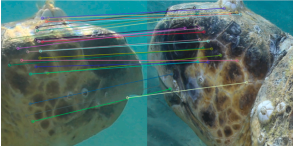
\includegraphics[width=0.5\linewidth]{bab2/face-scale.png}
	\caption{Persamaan pola di sisik kepala pada individu penyu yang sama \cite{papafitsoros2024facial}}
	\label{fig:face-scale}
\end{figure}

\subsubsection{Metode Ekstraksi Fitur Berbasis Citra Kepala}
 
Secara historis, ekstraksi fitur dari citra kepala penyu dilakukan menggunakan deskriptor fitur lokal seperti SIFT (\textit{Scale-Invariant Feature Transform}), SURF (\textit{Speeded-Up Robust Features}), atau ORB (\textit{Oriented FAST and Rotated BRIEF}) yang mendeteksi dan mendeskripsikan titik-titik kunci (\textit{keypoints}) pada tepi dan persimpangan sisik \cite{adam2023seaturtleid2022}. Metode-metode tersebut kemudian diimplementasikan dalam perangkat lunak khusus seperti APHIS \cite{gatto2018flipper} dan HotSpotter \cite{dunbar2023photo}.
 
Pendekatan berbasis \textit{deep learning} menggantikan ekstraksi fitur manual dengan representasi yang dipelajari secara otomatis dari data. CNN yang dilatih dengan \textit{transfer learning} dari ImageNet \cite{nguyen2023cnn} mampu mengekstraksi fitur hierarkis yang lebih kaya: lapisan-lapisan awal menangkap tepi dan tekstur sisik, sementara lapisan-lapisan dalam mengodekan pola geometris kompleks yang khas per individu. Pada arsitektur ViT \cite{dosovitskiy2021image}, mekanisme \textit{self-attention} memungkinkan model untuk secara serentak memperhatikan beberapa region sisik yang tersebar di seluruh kepala, sehingga menghasilkan representasi global yang lebih komprehensif dibandingkan CNN.

%-------------------------------------------------------------
\subsection{Vision Transformer}
%-------------------------------------------------------------
\textit{Vision Transformer} (ViT) merupakan arsitektur jaringan saraf yang diadaptasi dari arsitektur \textit{Transformer} yang semula dikembangkan untuk pemrosesan bahasa alami, kemudian diterapkan secara langsung pada data citra \cite{dosovitskiy2021image}. Dosovitskiy et al.\ menunjukkan bahwa sebuah \textit{Transformer} murni yang diterapkan pada urutan \textit{patch} citra mampu mencapai akurasi yang setara atau bahkan melampaui jaringan konvolusi (\textit{convolutional neural networks}, CNN) terbaik pada tugas klasifikasi citra, dengan catatan bahwa model dilatih pada data yang memadai dalam jumlah besar. Perbedaan mendasar ViT dengan CNN terletak pada tidak adanya \textit{inductive bias} spasial seperti lokalitas dan translasi-invariansi yang dimiliki konvolusi, sehingga ViT harus mempelajari hubungan spasial secara murni dari data.

\begin{figure}[H]
	\centering
	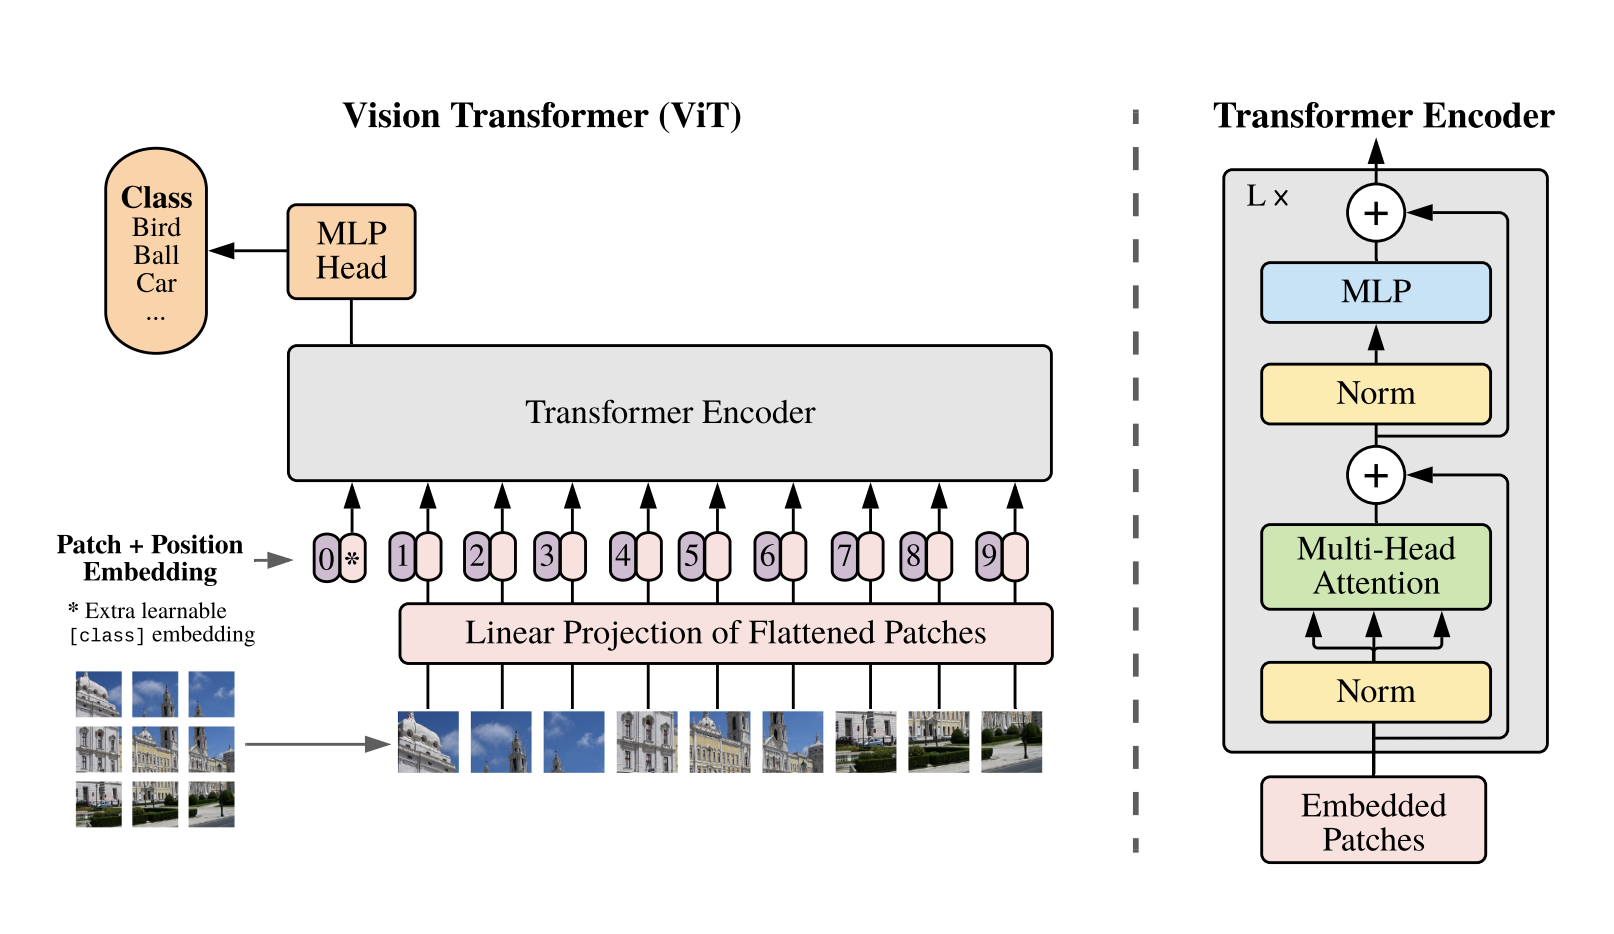
\includegraphics[width=0.9\linewidth]{bab2/vit-architecture.png}
	\caption{Arsitektur ViT: pembagian citra menjadi \textit{patch} sebelum diproses oleh lapisan \textit{transformer}. \cite{dosovitskiy2021image}}
	\label{fig:vit-architecture}
\end{figure}

%-------------------------------------------------------------
\subsection{Mekanisme Pembagian Patch}
%-------------------------------------------------------------
Citra masukan berukuran $H \times W \times C$ dibagi menjadi $N = \frac{H \cdot W}{P^2}$ \textit{patch} berukuran $P \times P$ piksel, di mana $P$ adalah ukuran \textit{patch}. Setiap \textit{patch} diratakan (\textit{flatten}) menjadi vektor berdimensi $P^2 \cdot C$, kemudian diproyeksikan secara linear ke dimensi laten $D$ menggunakan matriks proyeksi yang dapat dipelajari, sehingga menghasilkan urutan $N$ vektor \textit{embedding patch} \cite{dosovitskiy2021image}. Informasi posisi spasial setiap \textit{patch} ditambahkan melalui \textit{positional embedding} yang dapat dipelajari, agar model mengetahui lokasi relatif setiap \textit{patch} dalam citra asli.
 
Sebuah token kelas (\textit{class token}, \texttt{[CLS]}) yang dapat dipelajari ditambahkan di awal urutan, menghasilkan urutan total sepanjang $N+1$ token. Token ini tidak berkorespondensi dengan \textit{patch} citra mana pun, melainkan berinteraksi dengan seluruh \textit{patch} melalui \textit{self-attention} dan mengakumulasikan informasi global dari keseluruhan citra \cite{dosovitskiy2021image}. Setelah melewati seluruh blok \textit{Transformer}, keluaran dari token \texttt{[CLS]} inilah yang dimanfaatkan sebagai representasi global citra untuk tugas hilir, termasuk Re-ID. %Dalam penelitian ini, ukuran \textit{patch} $P = 16$ digunakan, sehingga untuk citra $256 \times 256$, model memproses urutan 257 token (256 \textit{patch} + 1 \texttt{[CLS]}).

\subsubsection{Blok Transformer dan Self-Attention}
 Setiap blok \textit{Transformer} dalam ViT terdiri dari dua sub-lapisan utama yang diapit oleh \textit{Layer Normalization} (LN) dan koneksi residual, yaitu: (1) \textit{Multi-Head Self-Attention} (MHSA) dan (2) \textit{Multi-Layer Perceptron} (MLP) dengan aktivasi GELU. Mekanisme \textit{self-attention} memungkinkan setiap token untuk mempertimbangkan kontribusi semua token lain dalam urutan secara global dan simultan, tanpa batasan jangkauan (\textit{receptive field}) seperti yang terdapat pada operasi konvolusi \cite{dosovitskiy2021image}.

Pada MHSA dengan $h$ \textit{head}, setiap token diproyeksikan menjadi tiga vektor Query ($Q$), Key ($K$), dan Value ($V$). Skor \textit{attention} antara setiap pasang token dihitung sebagai:
\begin{equation}
    \text{Attention}(Q, K, V)
    = \text{softmax}\!\left(\frac{QK^\top}{\sqrt{d_k}}\right) V
\end{equation}
di mana $d_k$ adalah dimensi tiap \textit{head}. Pemanfaatan beberapa \textit{head} secara paralel memungkinkan model untuk mempelajari pola relasi yang beragam secara simultan; misalnya, satu \textit{head} dapat belajar memperhatikan tepi sisik sementara \textit{head} lain memperhatikan pola warna. Kemampuan MHSA untuk memandang keseluruhan citra secara global pada setiap lapisan sangat relevan untuk Re-ID penyu, di mana pola diskriminatif tersebar di berbagai region sisik kepala yang tidak berdekatan.

%-------------------------------------------------------------
\subsection{Pra-pelatihan DINO}
%-------------------------------------------------------------
DINO (\textit{Self-DIstillation with NO labels}) adalah kerangka pra-pelatihan \textit{self-supervised} yang dirancang khusus untuk bersinergi dengan arsitektur \textit{Vision Transformer} \cite{caron2021dino}. \textit{Self-supervised learning} (SSL) adalah paradigma pelatihan di mana model belajar merepresentasikan data tanpa memerlukan anotasi label dari manusia, melainkan dengan memanfaatkan struktur inheren dari data itu sendiri sebagai sinyal supervisi. Keuntungan fundamental SSL adalah kemampuannya memanfaatkan dataset citra yang jauh lebih besar dibandingkan dataset berlabel, yang secara umum menghasilkan representasi yang lebih kaya dan lebih dapat digeneralisasi lintas domain. Keluarga DINO telah berkembang dari versi aslinya (DINO, 2021) hingga DINOv2 (2023) yang jauh lebih kuat, keduanya dikembangkan oleh Facebook AI Research (FAIR).
 
\subsubsection{DINO}
 
DINO diusulkan oleh Caron et al.\ \cite{caron2021dino} dengan tujuan untuk memahami apakah pelatihan \textit{self-supervised} dapat membangkitkan properti-properti unik yang tidak muncul ketika ViT dilatih secara \textit{supervised}. DINO menggunakan kerangka \textit{teacher-student self-distillation}: dua jaringan dengan arsitektur identik, yakni \textit{student} dan \textit{teacher}, secara bersamaan menerima \textit{crop} berbeda dari citra yang sama, dan model \textit{student} dilatih untuk mencocokkan distribusi keluaran \textit{softmax} dari model \textit{teacher}. Model \textit{teacher} tidak dilatih secara langsung, melainkan diperbarui sebagai \textit{exponential moving average} (EMA) dari bobot \textit{student}, sehingga tidak memerlukan label eksternal maupun \textit{negative pair} seperti yang digunakan dalam metode kontrastif.
 
Fungsi \textit{loss} DINO meminimalkan \textit{cross-entropy} antara distribusi keluaran \textit{student} dan \textit{teacher} pada pasangan \textit{global} dan \textit{local crop}:
\begin{equation}
    \mathcal{L}_{\text{DINO}}
    = -\sum_{x \in \{\text{global crops}\}}
      \sum_{\substack{x' \in \{\text{all crops}\} \\ x' \neq x}}
      P_s(x')\, \log P_t(x)
\end{equation}
di mana $P_s$ dan $P_t$ adalah distribusi \textit{softmax} yang dinormalisasi dari \textit{student} dan \textit{teacher} dengan parameter temperatur yang berbeda \cite{caron2021dino}.
 
Caron et al.\ \cite{caron2021dino} mengidentifikasi dua sifat \textit{emerging} yang penting: pertama, modul \textit{self-attention} pada blok terakhir secara eksplisit mengandung informasi mengenai tata letak skenario dan batas objek semantik, bahkan pada resolusi piksel, tanpa pernah diberikan label segmentasi; kedua, fitur yang dihasilkan merupakan \textit{k-NN classifier} yang sangat baik, mencapai 78{,}3\% akurasi top-1 pada ImageNet tanpa pelatihan lapisan klasifikasi apapun. Properti pertama sangat relevan untuk Re-ID penyu, karena kemampuan membedakan batas antar sisik kepala tanpa anotasi manual merupakan keunggulan yang signifikan mengingat tidak tersedianya dataset penyu berlabel segmentasi sisik secara individual.

\subsubsection{DINOv2}
 
DINOv2 diusulkan oleh Oquab et al.\ \cite{oquab2023dinov2} sebagai evolusi signifikan dari DINO yang menjawab dua kelemahan utamanya: keterbatasan skala data pelatihan dan inkonsistensi kualitas representasi antar tugas. Perbedaan utamanya terletak pada tiga aspek: (1) \textit{pipeline} kurasi data otomatis berbasis \textit{retrieval} yang membangun dataset LVD-142M, yakni 142 juta citra berkualitas tinggi dan beragam dari sumber web tanpa label; (2) teknik pelatihan gabungan yang mengombinasikan fungsi \textit{loss} DINO dengan komponen iBOT (\textit{image-level} dan \textit{patch-level self-distillation}) untuk menghasilkan fitur global dan lokal yang sama-sama kuat; serta (3) berbagai teknik stabilisasi pelatihan yang memungkinkan pelatihan pada skala besar tanpa divergensi \cite{oquab2023dinov2}.
 
Oquab et al.\ \cite{oquab2023dinov2} menunjukkan bahwa DINOv2 menghasilkan fitur visual serba guna (\textit{all-purpose visual features}) yang dapat digunakan secara langsung tanpa \textit{fine-tuning} untuk berbagai tugas, meliputi klasifikasi, deteksi objek, segmentasi semantik, hingga estimasi kedalaman monokuler. Pada hampir seluruh \textit{benchmark} yang diuji, DINOv2 melampaui metode \textit{self-supervised} sebelumnya dan bersaing dengan atau bahkan melampaui model yang dilatih secara \textit{weakly supervised} menggunakan data berskala web berlabel teks.
 
\subsubsection{DINOv3}
 
DINOv3 diperkenalkan oleh Sim\'{e}oni et al.\ \cite{simeoni2025dinov3} sebagai generasi lanjutan dari keluarga DINO yang berfokus pada peningkatan kualitas representasi visual universal untuk berbagai tugas \textit{computer vision}. Berbeda dengan DINOv2 yang menitikberatkan pada pembangunan fitur visual serbaguna melalui kombinasi \textit{image-level} dan \textit{patch-level self-distillation}, DINOv3 dikembangkan untuk menghasilkan representasi yang lebih stabil, lebih kaya secara semantik, dan lebih kuat dalam memahami struktur spasial lokal pada citra.
 
Seperti pendahulunya, DINOv3 tetap menggunakan paradigma \textit{teacher-student self-distillation} berbasis Vision Transformer (ViT), di mana model \textit{teacher} diperbarui menggunakan mekanisme EMA dari parameter \textit{student} \cite{simeoni2025dinov3}. Namun demikian, DINOv3 memperkenalkan berbagai penyempurnaan pada strategi pelatihan dan regularisasi sehingga mampu menghasilkan fitur yang lebih konsisten pada berbagai skala dan distribusi data. Sim\'{e}oni et al.\ \cite{simeoni2025dinov3} menunjukkan bahwa DINOv3 memiliki kemampuan \textit{dense feature extraction} yang sangat kuat, terutama dalam menghasilkan korespondensi spasial yang presisi antar bagian citra, serta menunjukkan kemampuan generalisasi yang lebih baik pada data di luar distribusi pelatihan (\textit{out-of-distribution generalization}).

%-------------------------------------------------------------
\subsection{Pembelajaran Metrik}
%-------------------------------------------------------------
Pembelajaran metrik (\textit{metric learning}) merupakan pendekatan pelatihan di mana model tidak dilatih untuk mengklasifikasikan masukan ke dalam kelas tetap, melainkan untuk mempelajari fungsi jarak yang mencerminkan kemiripan semantik antar sampel \cite{schroff2015facenet}. Fungsi \textit{loss} dalam pembelajaran metrik dirancang untuk secara eksplisit mengatur geometri ruang \textit{embedding}: mengecilkan jarak antar sampel dari kelas yang sama (\textit{intra-class compactness}) dan memperbesar jarak antar sampel dari kelas berbeda (\textit{inter-class separability}). Dalam konteks Re-ID \textit{open-set}, pendekatan ini jauh lebih tepat dibandingkan klasifikasi \textit{softmax} standar, karena model harus mampu menggeneralisasi ke identitas baru yang tidak dijumpai selama pelatihan, sesuatu yang tidak dapat dilakukan oleh kepala klasifikasi yang hanya memetakan ke kelas-kelas tetap.
 
\subsubsection{ArcFace Loss}
 
ArcFace (\textit{Additive Angular Margin Loss}) diusulkan oleh Deng et al.\ \cite{deng2019arcface} sebagai fungsi \textit{loss} yang secara geometris lebih bermakna dibandingkan pendekatan \textit{margin} sebelumnya seperti SphereFace dan CosFace. ArcFace beroperasi dalam ruang bola satuan (\textit{unit hypersphere}), di mana setiap \textit{embedding} dan setiap bobot prototipe kelas dinormalisasi L2 sehingga memiliki norma satu. Jarak antar \textit{embedding} dalam ruang ini sepenuhnya ditentukan oleh sudut $\theta$ di antara keduanya, dan ArcFace menambahkan margin sudut $m_a$ secara langsung pada sudut $\theta_{y_i}$ antara \textit{embedding} sampel dan bobot prototipe kelas yang benar:
\begin{equation}
    \mathcal{L}_{\text{ArcFace}}
    = -\frac{1}{N} \sum_{i=1}^{N}
      \log \frac{e^{s_a \cdot \cos(\theta_{y_i} + m_a)}}
                {e^{s_a \cdot \cos(\theta_{y_i} + m_a)}
                 + \displaystyle\sum_{j \neq y_i} e^{s_a \cdot \cos \theta_j}}
\end{equation}
Keunggulan geometris ArcFace terletak pada fakta bahwa margin $m_a$ beroperasi langsung dalam ruang sudut, sehingga berkorespondensi dengan jarak geodesik pada permukaan bola satuan dan memiliki interpretasi yang konsisten terlepas dari posisi kelas di ruang tersebut \cite{deng2019arcface}. Faktor skala $s_a$ memperbesar logit agar distribusi \textit{softmax} lebih terpusat dan gradiennya lebih informatif. ArcFace terbukti secara konsisten melampaui pendekatan \textit{margin} sebelumnya pada berbagai \textit{benchmark} pengenalan wajah.
 
\subsubsection{Triplet Loss dengan Online Hard Mining}
 
\textit{Triplet Loss} diusulkan oleh Schroff et al.\ \cite{schroff2015facenet} dalam sistem FaceNet sebagai cara untuk mengoptimalkan secara langsung jarak relatif antar pasangan sampel. \textit{Triplet Loss} bekerja pada triplet $(a, p, n)$ yang terdiri dari \textit{anchor} $a$, \textit{positive} $p$ (individu yang sama dengan \textit{anchor}), dan \textit{negative} $n$ (individu yang berbeda), dan meminimalkan:
\begin{equation}
    \mathcal{L}_{\text{Triplet}}
    = \frac{1}{N} \sum_{i=1}^{N}
      \max\!\left(d(a_i, p_i) - d(a_i, n_i) + m_t,\ 0\right)
\end{equation}
di mana $d(\cdot,\cdot)$ adalah jarak Euclidean dan $m_t$ adalah margin yang memaksa jarak positif lebih kecil dari jarak negatif dengan selisih minimum $m_t$. Hermans et al.\ \cite{hermans2017defense} mendemonstrasikan secara sistematis bahwa \textit{batch-hard mining}, yakni pemilihan pasangan \textit{positive} terjauh dan pasangan \textit{negative} terdekat dalam setiap \textit{batch}, menghasilkan gradien yang paling informatif dibandingkan semua strategi lainnya, termasuk pemilihan acak, \textit{semi-hard mining}, dan \textit{random hard mining}.
 
\subsubsection{Kombinasi ArcFace dan Triplet Loss}
 
Kombinasi kedua fungsi \textit{loss} secara linear memanfaatkan sifat komplementer yang mendasar: ArcFace mengoptimalkan separasi global antar semua kelas melalui bobot prototipe yang stabil, sementara \textit{Triplet Loss} mengoptimalkan konsistensi jarak lokal antar pasangan sampel nyata dalam setiap \textit{batch} secara adaptif \cite{deng2019arcface, schroff2015facenet}. Fungsi \textit{loss} total dirumuskan sebagai:
\begin{equation}
    \mathcal{L}_{\text{total}}
    = \mathcal{L}_{\text{ArcFace}} + \lambda_t \cdot \mathcal{L}_{\text{Triplet}}
\end{equation}
di mana $\lambda_t$ adalah bobot yang mengatur kontribusi relatif \textit{Triplet Loss}. Kombinasi ini mengatasi kelemahan masing-masing fungsi \textit{loss}: model secara bersamaan belajar batas keputusan yang tajam antar kelas pelatihan (dari ArcFace) dan struktur jarak yang baik untuk generalisasi ke identitas baru yang belum pernah dijumpai (dari \textit{Triplet Loss}). Strategi kombinasi \textit{loss} ini telah digunakan secara luas dalam sistem Re-ID kompetitif \cite{hermans2017defense} dan terbukti secara konsisten memberikan performa yang lebih baik dibandingkan penggunaan salah satu fungsi \textit{loss} secara tunggal.

%-------------------------------------------------------------
\subsection{Optimizer}
%-------------------------------------------------------------
Optimizer merupakan algoritma yang menentukan cara parameter model diperbarui pada setiap iterasi pelatihan berdasarkan gradien dari fungsi \textit{loss} \cite{kingma2015adam}. Tujuan utama optimizer adalah menemukan konfigurasi parameter yang meminimalkan fungsi \textit{loss} pada data pelatihan sekaligus mempertahankan kemampuan generalisasi pada data baru. Secara umum, aturan pembaruan parameter dinyatakan sebagai:
\begin{equation}
    \theta_{t+1} = \theta_t - \eta \cdot g(\nabla_\theta \mathcal{L})
\end{equation}
di mana $\theta_t$ adalah vektor parameter pada iterasi ke-$t$, $\eta$ adalah \textit{learning rate}, dan $g(\nabla_\theta \mathcal{L})$ adalah fungsi yang diterapkan optimizer terhadap gradien $\nabla_\theta \mathcal{L}$.

\subsubsection{AdamW}
 
AdamW (\textit{Adam with Decoupled Weight Decay}) diusulkan oleh Loshchilov dan Hutter \cite{loshchilov2019adamw} sebagai perbaikan atas Adam standar yang mengatasi masalah fundamental pada interaksi antara regularisasi dan pembaruan adaptif. Masalah utama Adam adalah bahwa regularisasi $L_2$ tidak ekuivalen dengan \textit{weight decay} pada algoritma adaptif: penambahan suku $L_2$ ke fungsi \textit{loss} menyebabkan efek regularisasi yang tidak merata, karena suku tersebut juga diskalakan oleh estimasi momen kedua. AdamW mengatasi permasalahan ini dengan memisahkan \textit{weight decay} sepenuhnya dari pembaruan adaptif gradien:
\begin{equation}
    \theta_{t+1}
    = \theta_t
      - \eta \cdot \left(
          \frac{\hat{m}_t}{\sqrt{\hat{v}_t} + \epsilon}
          + \lambda_w \cdot \theta_t
        \right)
\end{equation}
di mana $\hat{m}_t$ dan $\hat{v}_t$ adalah estimasi momen pertama dan kedua yang telah dikoreksi bias, $\lambda_w$ adalah koefisien \textit{weight decay}, dan $\epsilon$ adalah konstanta kecil untuk stabilitas numerik. Dengan cara ini, \textit{weight decay} selalu mengurangi bobot secara proporsional terhadap nilainya, terlepas dari besarnya gradien adaptif, sehingga menghasilkan regularisasi yang konsisten dan merata di seluruh parameter. Loshchilov dan Hutter \cite{loshchilov2019adamw} mendemonstrasikan bahwa AdamW menghasilkan generalisasi yang secara konsisten lebih baik dibandingkan Adam standar pada berbagai tugas, dengan perbedaan yang paling terasa pada model berbasis \textit{Transformer}.
 
\subsubsection{Layer-wise Learning Rate Decay (LLRD)}
 
Ketika melakukan \textit{fine-tuning} model pra-latih berskala besar seperti ViT-DINOv2, terdapat dilema fundamental antara dua kebutuhan yang bertentangan: memperbarui parameter secara agresif agar model beradaptasi dengan domain baru, dan mempertahankan representasi kaya yang telah dipelajari selama pra-pelatihan pada 142 juta citra. Pembaruan yang terlalu agresif dan merata pada seluruh lapisan berpotensi menghapus fitur-fitur representasi tingkat rendah yang sudah sangat baik, suatu fenomena yang dikenal sebagai \textit{catastrophic forgetting} \cite{sun2019bert}.
 
LLRD (\textit{Layer-wise Learning Rate Decay}) mengatasi dilema ini dengan memberikan \textit{learning rate} yang berbeda dan semakin kecil untuk lapisan-lapisan yang semakin dekat ke masukan \cite{sun2019bert}. Untuk blok \textit{Transformer} ke-$i$ dari total $L$ blok:
\begin{equation}
    \eta_i = \eta_{\text{bb}} \cdot \gamma^{L - i}
\end{equation}
di mana $\eta_{\text{bb}}$ adalah \textit{backbone base learning rate} dan $\gamma \in (0, 1)$ adalah faktor peluruhan per lapisan. Semakin kecil nilai $\gamma$, semakin besar perbedaan \textit{learning rate} antara lapisan terdalam dan lapisan teratas. Pendekatan ini pertama kali dipopulerkan dalam konteks \textit{fine-tuning} BERT \cite{sun2019bert} dan kemudian terbukti efektif pada ViT \cite{dosovitskiy2021image}.

%-------------------------------------------------------------
\subsection{Learning Rate Scheduler}
%-------------------------------------------------------------
\textit{Learning rate scheduler} (penjadwal \textit{learning rate}) merupakan komponen pelatihan yang mengatur nilai \textit{learning rate} $\eta$ secara dinamis sepanjang proses pelatihan, alih-alih mempertahankannya konstan \cite{loshchilov2017sgdr}. Motivasi utamanya bersumber dari sifat lanskap fungsi \textit{loss} jaringan saraf dalam yang sangat kompleks dan tidak konveks. Nilai $\eta$ yang besar diperlukan di awal pelatihan agar model dapat bergerak cepat melintasi \textit{plateau} dan menghindari minimum lokal yang dangkal, namun nilai yang sama besar di tahap akhir pelatihan menyebabkan model berosilasi di sekitar minimum dan gagal konvergen dengan tepat \cite{goyal2017accurate}. %Penelitian ini mengadopsi jadwal dua fase: \textit{linear warmup} pada epoch-epoch awal, diikuti oleh \textit{cosine decay} hingga akhir pelatihan.
 
\subsubsection{Linear Warmup}
 
\textit{Linear warmup} merupakan fase awal penjadwalan di mana nilai \textit{learning rate} dinaikkan secara bertahap dan linear dari nilai yang sangat kecil menuju nilai target $\eta_{\max}$ selama $W$ epoch pertama:
\begin{equation}
    \eta(e) = \eta_{\max} \cdot \frac{e + 1}{W},
    \quad e = 0, 1, \ldots, W-1
\end{equation}
Goyal et al.\ \cite{goyal2017accurate} mendemonstrasikan bahwa \textit{warmup} sangat penting ketika melatih dengan \textit{batch size} besar: tanpa \textit{warmup}, estimasi momen kedua Adam ($\hat{v}_t$) yang diinisialisasi nol belum stabil pada iterasi-iterasi awal, sehingga berpotensi menimbulkan pembaruan parameter yang besar dan tidak dapat diandalkan. Dalam konteks \textit{fine-tuning} ViT-DINOv2, \textit{warmup} memastikan bahwa model berangkat dari kondisi yang stabil sebelum \textit{learning rate} dinaikkan ke nilai penuhnya.
 
\subsubsection{Cosine Decay}
 
\textit{Cosine decay} (juga dikenal sebagai \textit{cosine annealing}) diperkenalkan oleh Loshchilov dan Hutter \cite{loshchilov2017sgdr} sebagai jadwal penurunan \textit{learning rate} yang halus setelah fase \textit{warmup}. Nilai $\eta$ diturunkan mengikuti setengah periode kurva kosinus dari $\eta_{\max}$ menuju 0:
\begin{equation}
    \eta(e)
    = \frac{\eta_{\max}}{2}
      \left(1 + \cos\!\left(\pi \cdot \frac{e - W}{E - W}\right)\right),
    \quad e = W, W+1, \ldots, E
\end{equation}
di mana $E$ adalah total jumlah epoch pelatihan. Berbeda dengan \textit{step decay} yang menurunkan \textit{learning rate} secara diskret dan mendadak pada interval tertentu, \textit{cosine decay} memberikan penurunan yang mulus dan monoton yang tidak mengejutkan model dengan perubahan $\eta$ yang tiba-tiba, sehingga memungkinkan konvergensi yang halus ke minimum yang baik \cite{loshchilov2017sgdr}.
 
%-------------------------------------------------------------
\subsection{Test-Time Augmentation}
%-------------------------------------------------------------
\textit{Test-Time Augmentation} (TTA) merupakan teknik inferensi yang menerapkan beberapa augmentasi berbeda pada citra saat pengujian, kemudian menggabungkan (\textit{aggregate}) prediksi dari seluruh versi teraugmentasi untuk memperoleh prediksi akhir yang lebih stabil dan akurat \cite{kim2020testa}. Berbeda dengan augmentasi pada fase pelatihan yang bertujuan mencegah \textit{overfitting}, TTA bertujuan mengurangi varians prediksi saat inferensi dengan memanfaatkan invarian yang seharusnya dimiliki model terhadap transformasi-transformasi tertentu.
 
TTA efektif karena dua alasan utama. Pertama, distribusi citra yang dijumpai saat inferensi seringkali memiliki variasi yang tidak sepenuhnya tercakup oleh augmentasi pelatihan, dan TTA memungkinkan model untuk memandang citra dari berbagai sudut pandang augmentasi secara serentak. Kedua, rata-rata prediksi dari beberapa transformasi secara statistik memiliki varians lebih rendah dibandingkan prediksi tunggal, karena galat acak dari masing-masing transformasi cenderung saling menghilangkan \cite{kim2020testa}.
 
Dalam konteks Re-ID berbasis \textit{embedding}, TTA diterapkan dengan menghasilkan beberapa vektor \textit{embedding} dari transformasi berbeda atas citra yang sama, misalnya \textit{flip} horizontal, \textit{center crop} dari ukuran berbeda, \textit{crop} dengan pergeseran posisi, dan perubahan kecerahan ringan, kemudian menggabungkan vektor-vektor tersebut melalui rata-rata dan normalisasi L2 menjadi satu representasi yang lebih \textit{robust}.

%-------------------------------------------------------------
\subsection{Aggregated Embedding}
%-------------------------------------------------------------
\textit{Aggregated embedding} merupakan teknik pengkodean representasi yang menggabungkan beberapa vektor \textit{embedding} dari sumber berbeda menjadi satu vektor tunggal yang lebih stabil, informatif, dan tahan terhadap variasi kondisi pengambilan gambar \cite{zhong2017reranking}. Teknik ini didasarkan pada prinsip bahwa sebuah identitas tidak dapat direpresentasikan secara optimal hanya oleh satu vektor yang berasal dari satu citra tunggal, karena setiap citra hanya menangkap sebagian kecil dari variasi visual yang mungkin terjadi. Dengan menggabungkan informasi dari beberapa sumber, representasi agregat memiliki cakupan distribusi yang jauh lebih luas dari variasi visual yang mungkin muncul saat inferensi.
 
Agregasi dapat dilakukan dalam dua dimensi yang saling melengkapi: (1) agregasi antar augmentasi dari satu citra yang sama (TTA), yang mengurangi sensitivitas terhadap variasi kondisi pengambilan gambar spesifik pada satu foto; dan (2) agregasi antar citra dari satu identitas yang sama dalam galeri, yang merangkum seluruh variasi penampakan individu tersebut yang telah terekam.
 
\subsubsection{Agregasi Antar Augmentasi}
 
Untuk setiap citra, baik \textit{query} maupun \textit{gallery}, diterapkan $T$ transformasi TTA yang berbeda. Model mengekstraksi satu vektor \textit{embedding} per transformasi, menghasilkan himpunan $\{e_1, e_2, \ldots, e_T\}$. Vektor-vektor tersebut kemudian dirata-rata dan dinormalisasi secara L2:
\begin{equation}
    \bar{e} = \frac{1}{T} \sum_{t=1}^{T} e_t,
    \qquad
    \tilde{e} = \frac{\bar{e}}{\|\bar{e}\|_2}
\end{equation}
Komponen-komponen yang berfluktuasi secara acak akibat variasi augmentasi cenderung saling menghilangkan dalam proses rata-rata, sementara komponen-komponen yang konsisten di semua transformasi, yakni komponen yang mencerminkan identitas individu diperkuat secara relatif \cite{kim2020testa}. Normalisasi L2 setelah rata-rata mengembalikan vektor ke permukaan bola satuan agar konsisten dengan ruang \textit{embedding} yang digunakan untuk komputasi kemiripan.
 
\subsubsection{Agregasi Antar Citra}
 
Pada data galeri, setiap identitas dapat memiliki lebih dari satu citra referensi yang diambil pada waktu, kondisi, dan sudut yang berbeda-beda. Setelah setiap citra galeri diproses dengan TTA untuk menghasilkan vektor yang telah diagregasi $\tilde{e}_j^{(k)}$ (vektor TTA-agregat dari citra ke-$j$ untuk identitas $k$), seluruh vektor dari identitas yang sama dirata-rata kembali dan dinormalisasi ulang:
\begin{equation}
    e_{\text{gallery}}^{(k)}
    = \frac{\displaystyle\sum_{j=1}^{M_k} \tilde{e}_j^{(k)}}
           {\left\|\displaystyle\sum_{j=1}^{M_k} \tilde{e}_j^{(k)}\right\|_2}
\end{equation}
di mana $M_k$ adalah jumlah citra galeri untuk identitas $k$. Hasilnya adalah satu vektor galeri per identitas yang merangkum informasi dari seluruh citra referensi lintas berbagai kondisi pengambilan gambar. Pendekatan ini secara substansial mengurangi pengaruh citra yang mengandung \textit{noise}, oklusi, atau kondisi pencahayaan ekstrem, karena kontribusi satu citra yang kurang representatif terdilusi oleh kontribusi citra-citra lain yang lebih baik \cite{zhong2017reranking}.

%-------------------------------------------------------------
\subsection{Cosine Similarity}
%-------------------------------------------------------------
\textit{Cosine similarity} merupakan ukuran kemiripan antara dua vektor yang mengukur kosinus sudut di antara keduanya dalam ruang berdimensi tinggi, tanpa mempertimbangkan magnitudo atau panjang vektor \cite{manning2008introduction}. Untuk dua vektor $\mathbf{u}, \mathbf{v} \in \mathbb{R}^d$, \textit{cosine similarity} didefinisikan sebagai:
\begin{equation}
    \text{sim}(\mathbf{u}, \mathbf{v})
    = \frac{\mathbf{u} \cdot \mathbf{v}}{\|\mathbf{u}\|_2 \cdot \|\mathbf{v}\|_2}
    = \cos\theta
\end{equation}
di mana $\theta$ adalah sudut antara dua vektor dalam ruang berdimensi $d$. Nilai \textit{cosine similarity} berkisar dari $-1$ (berlawanan arah sempurna) hingga $+1$ (searah sempurna), dengan nilai 0 mengindikasikan ortogonalitas. Berbeda dengan jarak Euclidean yang sensitif terhadap magnitudo vektor, \textit{cosine similarity} murni mengukur orientasi relatif di ruang vektor, menjadikannya sangat sesuai untuk membandingkan representasi yang telah dinormalisasi ke magnitudo seragam.
 
\subsubsection{Keunggulan dalam Ruang Embedding Ternormalisasi}
 
Ketika seluruh vektor \textit{embedding} telah dinormalisasi secara L2 sehingga $\|\mathbf{u}\|_2 = \|\mathbf{v}\|_2 = 1$, \textit{cosine similarity} menjadi identik dengan perkalian titik biasa (\textit{dot product}):
\begin{equation}
    \text{sim}(\mathbf{u}, \mathbf{v}) = \mathbf{u} \cdot \mathbf{v}
    \quad \text{jika } \|\mathbf{u}\|_2 = \|\mathbf{v}\|_2 = 1
\end{equation}
Kesetaraan ini memiliki implikasi komputasi yang signifikan: pencarian kemiripan antara seluruh vektor \textit{query} terhadap seluruh vektor \textit{gallery} dapat dinyatakan sebagai operasi perkalian matriks:
\begin{equation}
    S = Q \cdot G^\top, \quad S \in \mathbb{R}^{n_q \times n_g}
\end{equation}
di mana $Q \in \mathbb{R}^{n_q \times d_e}$ adalah matriks \textit{embedding query} dan $G \in \mathbb{R}^{n_g \times d_e}$ adalah matriks \textit{embedding gallery}. Operasi perkalian matriks ini dapat dieksekusi secara efisien menggunakan operasi BLAS yang teroptimasi pada GPU, memungkinkan komputasi kemiripan $n_q \times n_g$ pasang vektor dalam satu operasi tunggal tanpa perulangan eksplisit \cite{manning2008introduction}.
 
\subsubsection{Cosine Distance sebagai Ukuran Ketidakmiripan}
 
Dalam konteks pencarian dan perankingan, \textit{cosine distance} didefinisikan sebagai komplemen dari \textit{cosine similarity}:
\begin{equation}
    D_{\text{cosine}}(\mathbf{u}, \mathbf{v})
    = 1 - \text{sim}(\mathbf{u}, \mathbf{v})
    = 1 - \mathbf{u} \cdot \mathbf{v}
\end{equation}
Nilai \textit{cosine distance} berkisar dari 0 (identik dalam arah) hingga 2 (berlawanan arah sempurna). Dalam sistem Re-ID, daftar kandidat identitas untuk setiap \textit{query} dihasilkan dengan mengurutkan entri galeri berdasarkan \textit{cosine distance} secara menaik, atau ekuivalennya, berdasarkan \textit{cosine similarity} secara menurun \cite{zheng2015scalable}. Terdapat pula hubungan langsung antara \textit{cosine distance} dan jarak Euclidean pada vektor ternormalisasi L2: $\|\mathbf{u} - \mathbf{v}\|_2^2 = 2(1 - \mathbf{u} \cdot \mathbf{v}) = 2 \cdot D_{\text{cosine}}(\mathbf{u}, \mathbf{v})$, yang berarti perankingan menggunakan keduanya menghasilkan urutan yang identik.

%-------------------------------------------------------------
\subsection{K-Reciprocal Re-Ranking}
%-------------------------------------------------------------
Re-ranking dengan \textit{k-reciprocal encoding} diusulkan oleh Zhong et al.\ \cite{zhong2017reranking} sebagai langkah pasca-pemrosesan untuk meningkatkan akurasi hasil pencarian. Gagasan dasarnya adalah: apabila dua sampel saling menjadi tetangga terdekat satu sama lain (\textit{k-reciprocal neighbors}), besar kemungkinan keduanya berasal dari identitas yang sama. Jarak akhir dikombinasikan secara linear antara jarak kosinus awal dan jarak Jaccard yang dihitung dari \textit{k-reciprocal encoding}:
\begin{equation}
    D_{\text{final}}(q, g)
    = \lambda_{\text{rr}} \cdot D_{\text{cosine}}(q, g)
    + (1 - \lambda_{\text{rr}}) \cdot D_{\text{Jaccard}}(q, g)
\end{equation}
Metode ini bersifat \textit{unsupervised} dan terbukti meningkatkan performa secara signifikan tanpa memerlukan data berlabel tambahan \cite{zhong2017reranking}.

%-------------------------------------------------------------
\subsection{Metrik Evaluasi}
%-------------------------------------------------------------
\subsubsection{Cumulative Matching Characteristic (CMC)}
 
CMC mengukur persentase \textit{query} yang identitas benarnya ditemukan dalam $k$ kandidat teratas. Rank-1 (R@1) merupakan metrik terpenting karena mencerminkan kemampuan identifikasi langsung tanpa intervensi manusia. Rank-5 (R@5) dan Rank-10 (R@10) mengukur toleransi sistem dalam skenario di mana beberapa kandidat teratas perlu diperiksa \cite{zheng2015scalable}.
 
\subsubsection{Mean Average Precision (mAP)}
 
mAP menghitung rata-rata \textit{Average Precision} (AP) di seluruh \textit{query}. AP mempertimbangkan posisi seluruh citra galeri yang relevan dalam daftar peringkat, bukan hanya yang pertama. mAP bersifat lebih informatif dibandingkan Rank-1 ketika galeri memiliki banyak citra per identitas, karena mengukur kemampuan model dalam menempatkan semua kecocokan yang benar secara konsisten pada posisi teratas hasil pencarian \cite{zheng2015scalable}.
\cleardoublepage
\chapter{METODOLOGI}
\label{sec:chap3_metodologi}

Penelitian ini dirancang dengan menggunakan serangkaian metode yang sistematis guna mencapai hasil re-identifikasi penyu laut yang akurat dan dapat digeneralisasi. Alur metodologi secara keseluruhan diilustrasikan melalui diagram berikut.

\begin{figure}[H]
    \centering
    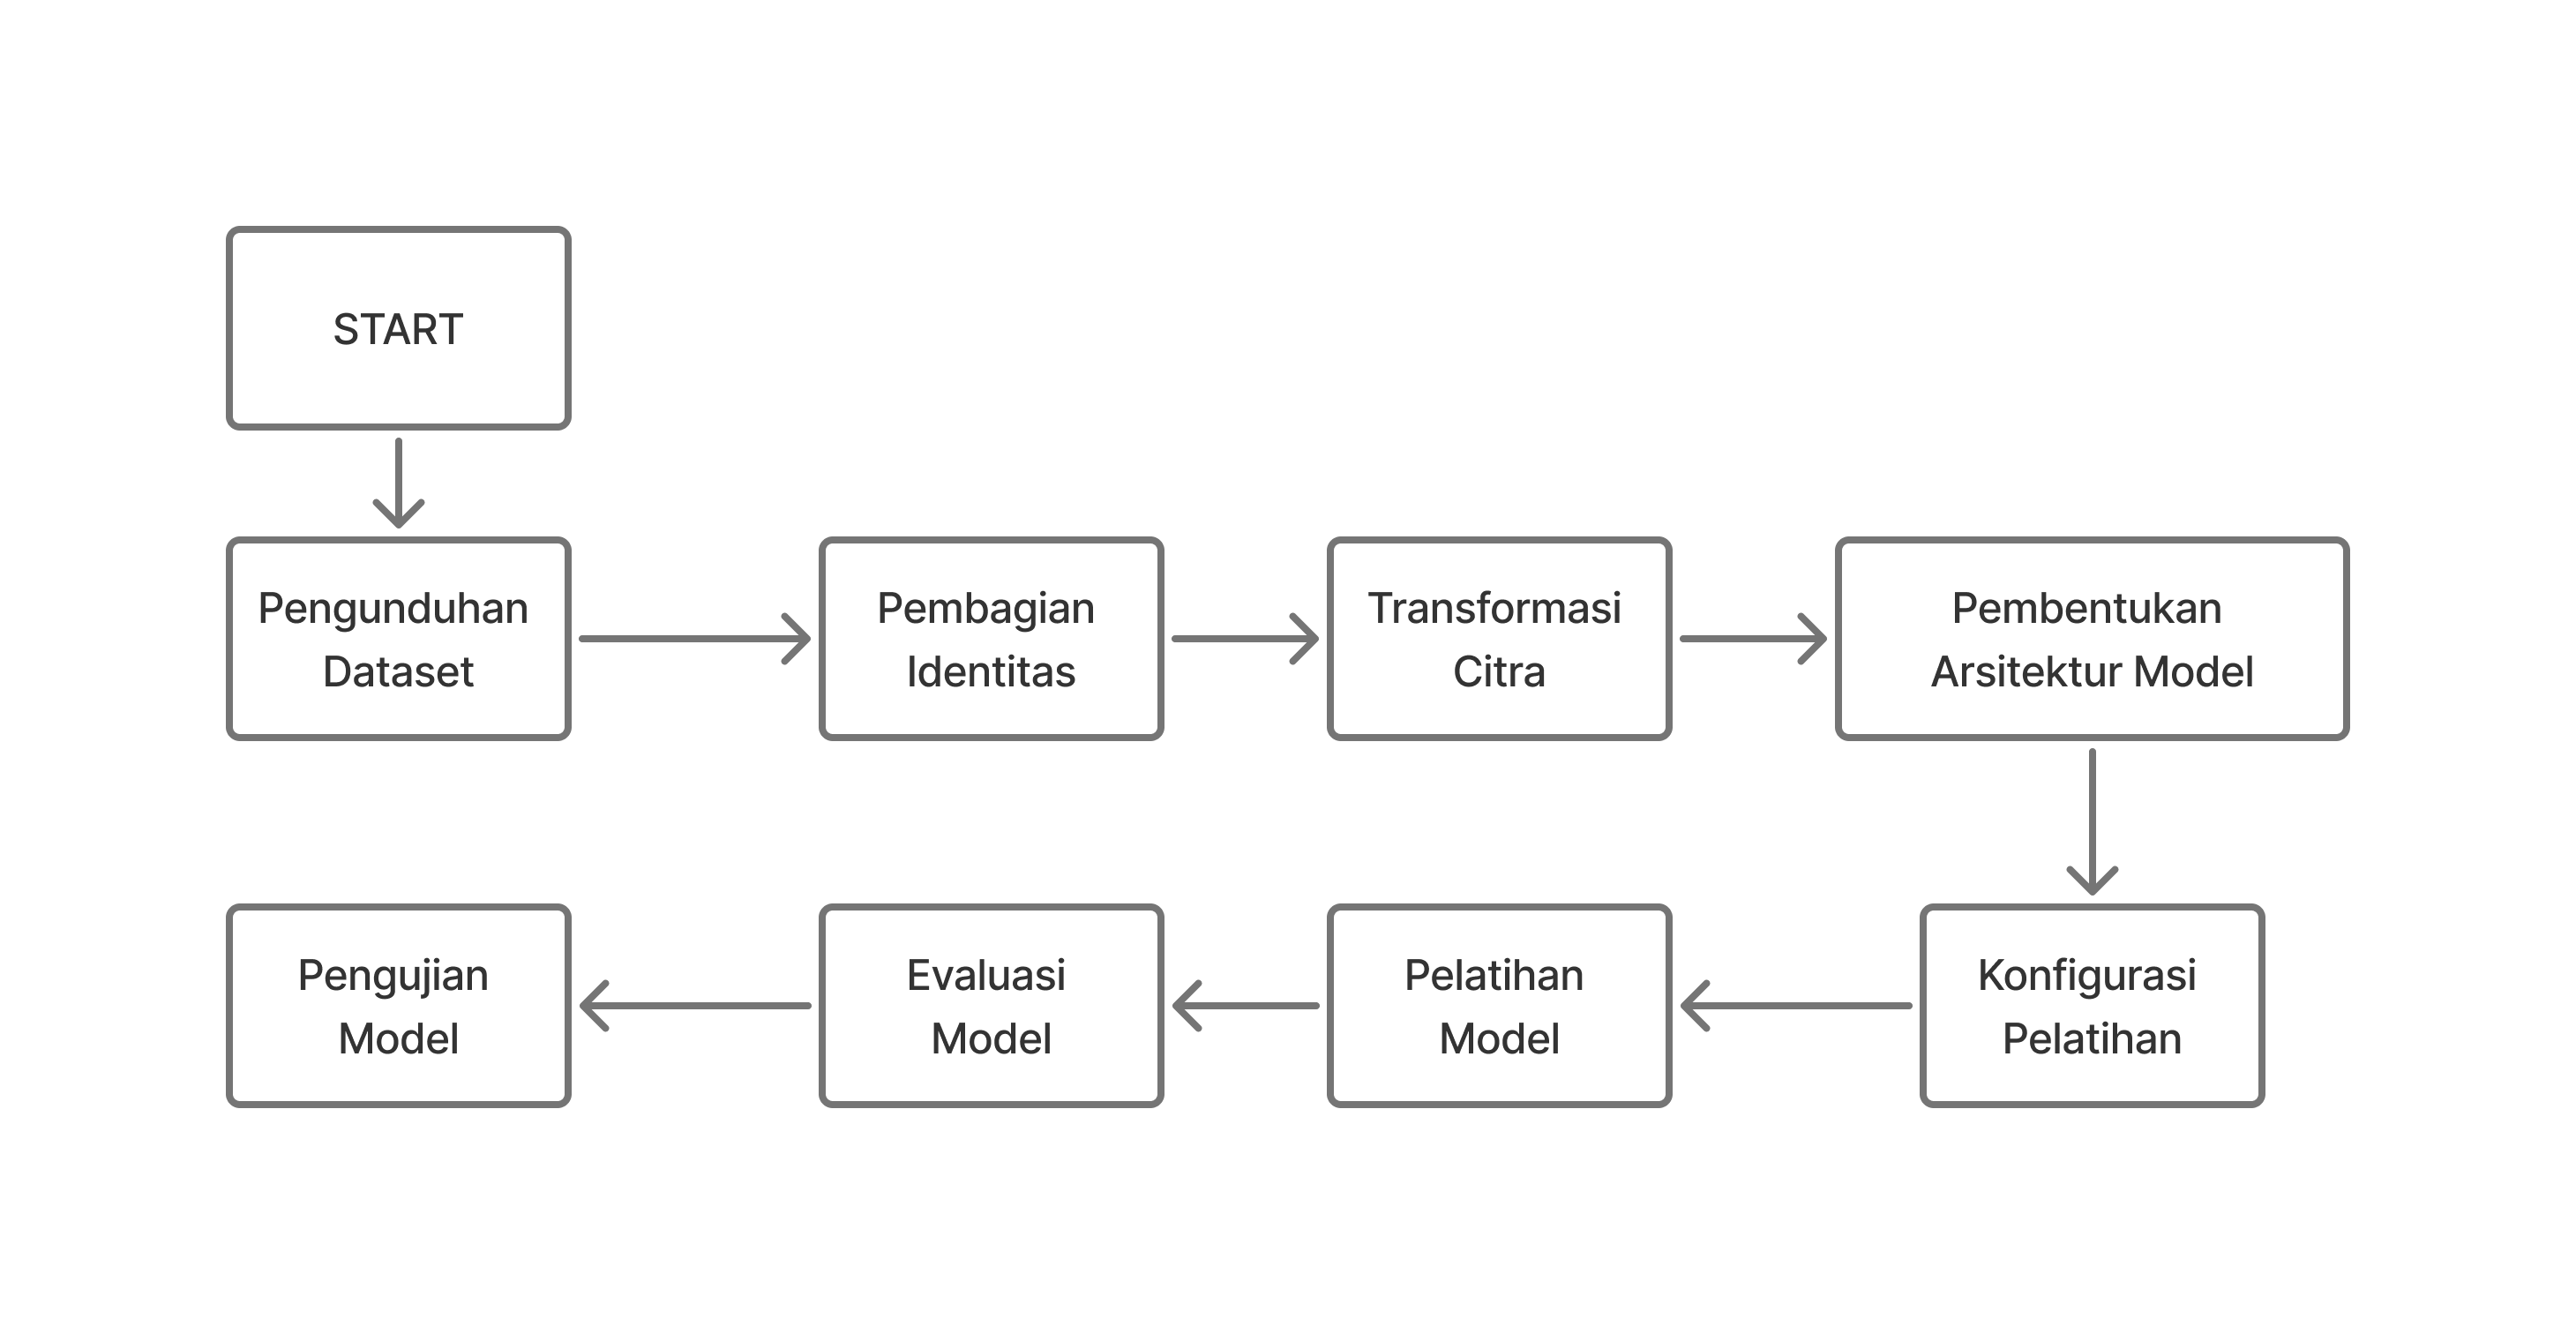
\includegraphics[width=0.9\linewidth]{bab3/diagram.png}
    \caption{Blok Diagram Pembangunan Model}
    \label{fig:diagram-block}
\end{figure}


\section{Dataset}
\subsection{Dataset SeaTurtleIDHeads}

Penelitian ini menggunakan dataset publik yang bernama \textit{SeaTurtleIDHeads}. Dataset \textit{SeaTurtleIDHeads} merupakan kumpulan data yang dirancang secara khusus untuk keperluan penelitian re-identifikasi individu penyu laut berdasarkan pola unik pada bagian kepala dan sisik mereka. Dataset ini banyak dimanfaatkan dalam bidang \textit{computer vision}, kecerdasan buatan, dan konservasi satwa liar, mengingat setiap individu penyu memiliki pola sisik kepala yang unik dan persisten sepanjang masa hidupnya, sebagaimana sidik jari pada manusia.

\begin{figure}[H]
    \centering
    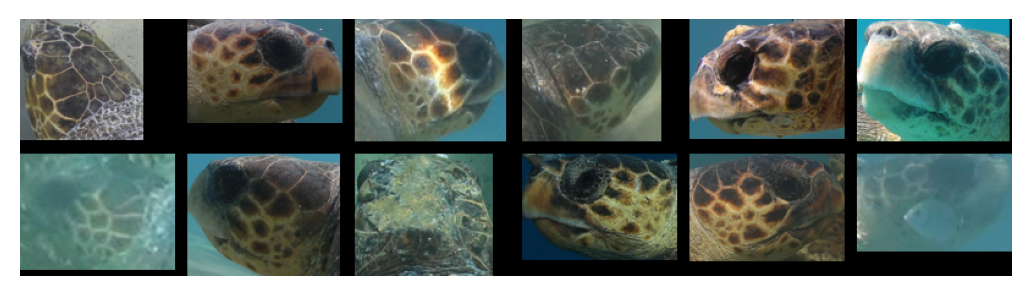
\includegraphics[width=0.9\linewidth]{bab3/SeaTurtleIDHeads.png}
    \caption{Sampel dataset SeaTurtleIDHeads \cite{wildlifedatasets_seaturtleidheads}}
    \label{fig:SeaTurtleIDHeads-sample}
\end{figure}

Dataset \textit{SeaTurtleIDHeads} memuat 7.582 citra dari 400 individu penyu laut yang dikumpulkan selama lebih dari satu dekade. Seluruh citra dalam dataset ini difokuskan pada bagian kepala penyu sehingga sesuai untuk digunakan dalam aplikasi identifikasi individu. Dataset ini memiliki variasi yang kaya dalam hal pose, pencahayaan, sudut pengambilan gambar, jarak kamera, dan resolusi citra, yang mencerminkan kondisi pengambilan foto secara nyata di lapangan. Variasi tersebut menjadi tantangan sekaligus peluang bagi model untuk mempelajari fitur yang benar-benar representatif terhadap identitas setiap individu.

Penelitian ini memilih \textit{SeaTurtleIDHeads} sebagai sumber data pelatihan dan validasi karena dataset ini menunjukkan keunggulan pada tugas re-identifikasi dibandingkan dengan anggota keluarga dataset yang sama, yaitu \textit{SeaTurtleID2022}. Dataset \textit{SeaTurtleID2022} memiliki resolusi citra yang lebih rendah dan dirancang terutama untuk tugas segmentasi, sehingga kurang ideal sebagai basis pelatihan bagi sistem re-identifikasi berbasis \textit{metric learning}.

\section{Pra-pemrosesan dan Augmentasi Data}
\subsection{Pembagian Dataset}

Dataset \textit{SeaTurtleIDHeads} dibagi menjadi tiga partisi menggunakan metode \textit{open-set identity split} dengan rasio 70:20:10, yang terdiri atas data pelatihan, data validasi, dan data pengujian. Pembagian dilakukan berdasarkan identitas individu sehingga tidak terdapat individu penyu yang sama pada lebih dari satu partisi. Hal ini memastikan bahwa evaluasi dilakukan terhadap identitas yang sepenuhnya belum pernah dilihat oleh model selama proses pelatihan (\textit{open-set evaluation}).

Sebelum pembagian dilakukan, identitas yang memiliki jumlah citra di bawah nilai minimum $N_{\min} = N_{\text{gallery}} + 2$ disaring dan dikeluarkan dari dataset. Persyaratan minimum tersebut memastikan bahwa setiap identitas memiliki citra yang cukup untuk dialokasikan ke galeri dan setidaknya dua citra ke \textit{query set}. Nilai parameter $N_{\text{gallery}}$ (yaitu $N_G$) merupakan salah satu variabel yang diuji dalam penelitian ini dan diuraikan lebih lanjut pada bab pengujian.

Data validasi dan data pengujian masing-masing dibagi lebih lanjut menjadi \textit{gallery set} dan \textit{query set}. Sebanyak $N_G$ citra per identitas dialokasikan ke galeri secara acak menggunakan \textit{random per-identity shuffle}, sementara sisa citra dialokasikan sebagai \textit{query}. Data validasi digunakan semata-mata untuk keperluan \textit{early stopping} dan pemilihan \textit{checkpoint} terbaik, sedangkan data pengujian hanya digunakan satu kali pada tahap evaluasi akhir.

\subsection{Transformasi Citra}

Seluruh citra diubah ukurannya menjadi $\mathit{img\_size} \times \mathit{img\_size}$ piksel sebelum dimasukkan ke dalam model. Nilai acuan $\mathit{img\_size} = 256$ digunakan sebagai \textit{baseline} dan merupakan salah satu variabel yang diuji dalam penelitian ini.

Pada fase pelatihan, diterapkan serangkaian augmentasi data yang berfungsi sebagai regularisasi implisit sekaligus meningkatkan kemampuan generalisasi model terhadap variasi kondisi pengambilan gambar. Augmentasi yang diterapkan meliputi hal-hal berikut.

\begin{itemize}
    \item \textbf{\textit{Random Crop}}: Citra diubah ukurannya menjadi $(\mathit{img\_size} + 32) \times (\mathit{img\_size} + 32)$ piksel, kemudian dipotong secara acak ke ukuran $\mathit{img\_size} \times \mathit{img\_size}$ piksel guna mensimulasikan variasi \textit{framing} dan posisi subjek.
    \item \textbf{\textit{Random Horizontal Flip}}: Citra dibalik secara horizontal dengan probabilitas 0,5, mengingat penyu dapat difoto dari sisi kiri maupun sisi kanan.
    \item \textbf{\textit{Color Jitter}}: Variasi acak diterapkan pada kecerahan, kontras, saturasi, dan \textit{hue} untuk mensimulasikan perbedaan kondisi pencahayaan bawah air.
    \item \textbf{\textit{Random Grayscale}}: Konversi citra ke format \textit{grayscale} dilakukan dengan probabilitas 0,1 untuk mendorong model agar tidak terlalu bergantung pada informasi warna.
    \item \textbf{\textit{Random Rotation}}: Rotasi acak diterapkan hingga 20 derajat guna mensimulasikan variasi sudut kamera.
    \item \textbf{\textit{Gaussian Blur}}: \textit{Blur} diterapkan menggunakan kernel berukuran $5 \times 5$ dengan nilai sigma acak antara 0,1 hingga 2,0 untuk mensimulasikan variasi fokus kamera.
    \item \textbf{\textit{Random Erasing}}: Area berbentuk persegi panjang dihapus secara acak pada citra dengan probabilitas 0,3 guna mensimulasikan oklusi parsial yang disebabkan oleh tumbuhan laut, bayangan, atau penghalang lainnya.
\end{itemize}

Pada fase evaluasi dan pengujian, hanya dilakukan operasi \textit{resize} dan normalisasi tanpa augmentasi acak agar hasil evaluasi bersifat deterministik dan dapat direproduksi.

Seluruh nilai piksel dinormalisasi menggunakan nilai rata-rata $\mu = (0{,}485,\ 0{,}456,\ 0{,}406)$ dan standar deviasi $\sigma = (0{,}229,\ 0{,}224,\ 0{,}225)$, yang merupakan statistik dari dataset ImageNet dan sesuai dengan statistik yang digunakan pada saat pra-pelatihan DINOv2.

\section{Arsitektur Model}

\subsection{Model Utama}

Arsitektur utama yang digunakan dalam penelitian ini adalah \textit{Vision Transformer} (ViT) yang telah dipra-latih menggunakan metode \textit{self-supervised learning} DINOv2. Model ini dimuat dari pustaka \textit{PyTorch Image Models} (timm). Model acuan yang digunakan adalah varian \textit{base}. Pada bab pengujian, akan dilakukan pelatihan menggunakan model lain dalam keluarga arsitektur yang sama.

ViT membagi citra masukan menjadi \textit{patch} berukuran $16 \times 16$ piksel. Untuk citra berukuran $256 \times 256$ piksel, terdapat $16 \times 16 = 256$ \textit{patch}. Setiap \textit{patch} diproyeksikan menjadi sebuah vektor dan diproses secara berurutan oleh 12 blok \textit{transformer}. Model ini menghasilkan keluaran berupa \textit{class token} berdimensi 768 yang merangkum representasi global dari keseluruhan citra.

DINOv2 dipilih sebagai metode pra-pelatihan karena terbukti menghasilkan representasi visual yang sangat kuat dan dapat ditransfer secara luas lintas domain tanpa memerlukan data berlabel. Pra-pelatihan berbasis \textit{self-distillation} ini mendorong model untuk mempelajari fitur semantik tingkat tinggi yang bersifat lokal maupun global, yang sangat relevan untuk tugas re-identifikasi di mana perbedaan antarindividu dapat bersifat sangat halus.

\subsection{Embedding Head}

Keluaran \textit{backbone} berupa vektor berdimensi 768 diproyeksikan ke dimensi \textit{embedding} yang lebih rendah menggunakan \textit{embedding head}. \textit{Head} ini terdiri atas tiga komponen yang diterapkan secara berurutan sebagai berikut.

\begin{enumerate}
    \item \textbf{\textit{Layer Normalization}}: Menormalisasi distribusi aktivasi dari \textit{backbone} sebelum proyeksi dilakukan. Langkah ini menstabilkan skala fitur yang masuk ke lapisan linear.
    \item \textbf{\textit{Dropout}}: Diterapkan dengan probabilitas $p_{\text{drop}}$ sebagai mekanisme regularisasi. Nilai acuan yang digunakan adalah $p_{\text{drop}} = 0{,}1$ dan merupakan salah satu variabel yang diuji dalam penelitian ini.
    \item \textbf{Proyeksi Linear}: Transformasi linear tanpa bias dari dimensi 768 ke dimensi \textit{embedding} $d_e$. Nilai acuan yang digunakan adalah $d_e = 256$ dan merupakan salah satu variabel yang diuji. Nilai ini dipilih karena proyeksi dengan dimensi 768$\rightarrow$768 tidak memberikan kompresi yang bermakna sehingga \textit{head} tidak dapat mempelajari representasi baru yang lebih diskriminatif.
\end{enumerate}

Setelah melewati \textit{head}, vektor dinormalisasi secara L2 sehingga seluruh \textit{embedding} berada pada permukaan \textit{unit hypersphere}. Normalisasi L2 tersebut memungkinkan penggunaan \textit{cosine similarity} yang setara dengan operasi perkalian titik, sehingga menyederhanakan proses perbandingan vektor pada tahap pengujian.

\subsection{ArcFace Loss}

ArcFace Loss digunakan sebagai fungsi \textit{loss} utama untuk pembelajaran separasi antaridentitas. ArcFace bekerja dengan menambahkan margin sudut $m_a$ pada sudut antara \textit{embedding} sampel dan bobot prototipe kelasnya di ruang bola satuan, sebelum penskalaan dengan faktor $s_a$ dan komputasi \textit{cross-entropy loss}.

Formulasi ArcFace Loss adalah sebagai berikut:
\begin{equation}
    \mathcal{L}_{\text{ArcFace}} = -\frac{1}{N} \sum_{i=1}^{N} \log \frac{e^{s_a \cdot \cos(\theta_{y_i} + m_a)}}{e^{s_a \cdot \cos(\theta_{y_i} + m_a)} + \sum_{j \neq y_i} e^{s_a \cdot \cos \theta_j}}
\end{equation}
di mana $\theta_{y_i}$ merupakan sudut antara \textit{embedding} sampel ke-$i$ dan bobot kelas yang benar $y_i$. Margin $m_a$ mendorong model untuk meningkatkan jarak sudut antara \textit{embedding} intra-kelas dan inter-kelas sehingga menghasilkan batas keputusan yang lebih tegas.

Pemilihan ArcFace dalam penelitian ini didasarkan pada beberapa pertimbangan. Pertama, sifat geometrisnya yang beroperasi pada bola satuan selaras dengan normalisasi L2 yang diterapkan pada keluaran \textit{embedding head}, sehingga seluruh proses pelatihan dan inferensi berlangsung dalam ruang yang konsisten secara geometris. Kedua, ArcFace telah terbukti efektif pada tugas re-identifikasi penyu secara spesifik, sebagaimana digunakan pada sistem \textit{baseline} \textit{SeaTurtleID2022} \cite{adam2023seaturtleid2022} maupun pada \textit{foundation model} MegaDescriptor \cite{cermak2024wildlifedatasets}, sehingga hasil yang diperoleh dapat dibandingkan secara langsung dengan penelitian terdahulu. Ketiga, kemampuan ArcFace dalam mempelajari representasi yang sangat diskriminatif dari kelas-kelas pelatihan sangat krusial mengingat perbedaan pola sisik antarindividu penyu dapat bersifat sangat halus.

Parameter yang diuji pada komponen ini adalah skala ArcFace $s_a$ dengan nilai acuan 64,0 dan margin ArcFace $m_a$ dengan nilai acuan 0,5.

\subsection{Online Hard Triplet Loss}

\textit{Triplet Loss} digunakan untuk memperkuat struktur lokal ruang \textit{embedding} melalui pembelajaran hubungan jarak relatif antarsampe. Setiap \textit{triplet} terdiri atas sebuah \textit{anchor} $a$, sebuah \textit{positive} $p$ (individu yang sama dengan \textit{anchor}), dan sebuah \textit{negative} $n$ (individu yang berbeda). Fungsi \textit{loss} ini mendorong terpenuhinya kondisi $d(a,p) + \text{margin} < d(a,n)$:

\begin{equation}
    \mathcal{L}_{\text{Triplet}} = \frac{1}{N} \sum_{i=1}^{N} \max\!\left(d(a_i, p_i) - d(a_i, n_i) + m_t,\ 0\right)
\end{equation}
di mana $d(\cdot, \cdot)$ adalah jarak Euclidean dan $m_t$ adalah margin \textit{triplet}.

Penelitian ini menggunakan strategi \textit{online hard mining}, di mana untuk setiap sampel dalam \textit{batch} dipilih \textit{positive} yang paling jauh (\textit{hardest positive}) dan \textit{negative} yang paling dekat (\textit{hardest negative}). Implementasi menggunakan \texttt{masked\_fill} untuk mengisolasi pasangan yang relevan, sehingga menghindari galat di mana nilai nol dari sampel yang bukan pasangan positif secara keliru terpilih sebagai jarak positif terkecil.

Parameter yang diuji pada komponen ini adalah margin \textit{triplet} $m_t$ dengan nilai acuan 0,3 dan bobot \textit{triplet} $\lambda_t$ dalam kombinasi \textit{loss} total dengan nilai acuan 0,5.

\subsection{Fungsi Loss Total}

Kedua fungsi \textit{loss} dikombinasikan secara linear sebagai berikut:

\begin{equation}
    \mathcal{L}_{\text{total}} = \mathcal{L}_{\text{ArcFace}} + \lambda_t \cdot \mathcal{L}_{\text{Triplet}}
\end{equation}
di mana $\lambda_t$ adalah bobot \textit{triplet}. Kombinasi ini memanfaatkan kelebihan masing-masing fungsi: ArcFace memberikan separasi global antarseluruh kelas yang terdefinisi di ruang proyeksi, sementara \textit{Triplet Loss} memperkuat konsistensi jarak lokal antara pasangan individu yang sama maupun berbeda pada setiap \textit{batch}.

\section{Konfigurasi Pelatihan}
\subsection{Balanced Batch Sampler}

Guna memastikan setiap \textit{batch} selalu memuat pasangan positif yang valid bagi \textit{Triplet Loss}, digunakan \textit{Balanced Batch Sampler}. Setiap \textit{batch} dibentuk dengan mengambil $P$ identitas secara acak, kemudian mengambil $K$ citra per identitas secara acak dengan penggantian (\textit{sampling with replacement}), sehingga ukuran \textit{batch} total adalah $P \times K$.

Nilai acuan yang digunakan adalah $P = 16$ identitas dan $K = 4$ citra per identitas, sehingga menghasilkan ukuran \textit{batch} sebesar 64. Nilai $P$ dan $K$ merupakan variabel yang diuji dalam penelitian ini. Identitas yang memiliki jumlah citra kurang dari $K$ dikeluarkan dari \textit{sampler} untuk menjaga konsistensi ukuran \textit{batch}.

Strategi ini lebih efektif dibandingkan dengan \textit{random sampling} konvensional, terutama pada dataset yang tidak seimbang. Dengan \textit{random sampling}, terdapat kemungkinan suatu \textit{batch} tidak memuat pasangan positif yang cukup, sehingga \textit{Triplet Loss} menjadi tidak informatif.

\subsection{AdamW dengan Layer-wise Learning Rate Decay}

Optimisasi dilakukan menggunakan AdamW dengan \textit{weight decay} $\lambda_w$ (nilai acuan: $10^{-4}$). AdamW dipilih karena memisahkan \textit{weight decay} dari pembaruan adaptif gradien, sehingga memberikan regularisasi yang lebih konsisten dibandingkan dengan Adam standar.

AdamW dikombinasikan dengan \textit{Layer-wise Learning Rate Decay} (LLRD) untuk melindungi representasi yang telah dipelajari selama pra-pelatihan DINOv2. LLRD memberikan \textit{learning rate} yang berbeda untuk setiap lapisan: lapisan yang lebih dalam (dekat dengan masukan) mendapatkan \textit{learning rate} yang lebih kecil, sedangkan lapisan yang lebih dekat ke keluaran mendapatkan \textit{learning rate} yang lebih besar.

Secara konkret, \textit{learning rate} untuk blok \textit{transformer} ke-$i$ (dari total $L = 12$ blok) dihitung menggunakan persamaan berikut:
\begin{equation}
    \eta_i = \eta_{\text{bb}} \cdot \gamma^{L - i}
\end{equation}
di mana $\eta_{\text{bb}}$ adalah \textit{backbone base learning rate} dan $\gamma$ adalah faktor peluruhan per lapisan. \textit{Embedding head} dan lapisan ArcFace menggunakan \textit{base learning rate} $\eta_{\text{base}}$ yang lebih tinggi, karena lapisan-lapisan tersebut diinisialisasi secara acak dan perlu belajar dengan laju yang lebih cepat.

Ketiga parameter tersebut, yaitu $\eta_{\text{base}}$, $\eta_{\text{bb}}$, dan $\gamma$, merupakan variabel yang diuji dalam penelitian ini dengan nilai acuan masing-masing sebesar $10^{-3}$, $10^{-5}$, dan $0{,}75$.

\subsection{Learning Rate Scheduler}

\textit{Learning rate scheduler} mengimplementasikan \textit{LambdaLR} yang membagi proses pelatihan menjadi dua fase berdasarkan fungsi skala $\lambda(e)$ terhadap \textit{epoch} $e$:

\begin{equation}
    \lambda(e) = \begin{cases}
        \dfrac{e + 1}{W} & \text{jika } e < W \quad \text{(fase \textit{warmup})} \\[10pt]
        \dfrac{1}{2}\!\left(1 + \cos\!\left(\pi \cdot \dfrac{e - W}{E - W}\right)\right) & \text{jika } e \geq W \quad \text{(fase \textit{cosine decay})}
    \end{cases}
\end{equation}
di mana $W$ adalah jumlah \textit{warmup epoch} dan $E$ adalah total jumlah \textit{epoch} pelatihan.

Pada fase \textit{warmup}, skala \textit{learning rate} meningkat secara linear dari $\frac{1}{W}$ menuju 1 selama $W$ \textit{epoch} pertama. Tujuannya adalah mencegah pembaruan gradien yang terlalu besar di awal pelatihan yang berpotensi merusak representasi DINOv2 sebelum \textit{embedding head} dan ArcFace mencapai kondisi yang stabil.

Pada fase \textit{cosine decay}, skala menurun dari 1 menuju 0 mengikuti kurva kosinus, sehingga memberikan penurunan \textit{learning rate} yang halus dan mencegah osilasi di sekitar titik minimum.

\subsection{Parameter Pelatihan Lainnya}

\begin{itemize}
    \item \textbf{\textit{Gradient Clipping}}: Norma gradien dibatasi pada nilai maksimum $G_{\max}$ (nilai acuan: 1,0) untuk menjaga stabilitas pelatihan dan mencegah terjadinya \textit{exploding gradient}.
    \item \textbf{Frekuensi Evaluasi}: Evaluasi pada data validasi dilaksanakan setiap 5 \textit{epoch}, bukan setiap \textit{epoch}, demi efisiensi komputasi.
    \item \textbf{\textit{Early Stopping}}: Proses pelatihan dihentikan lebih awal apabila tidak terdapat peningkatan nilai \textit{rank-1} pada data validasi selama $P_{\text{stop}}$ interval evaluasi berturut-turut (nilai acuan: 10 interval, setara dengan 50 \textit{epoch} tanpa peningkatan). \textit{Checkpoint} yang disimpan adalah model dengan nilai \textit{rank-1} validasi tertinggi.
    \item \textbf{\textit{Mixed Precision}}: Pelatihan menggunakan \textit{automatic mixed precision} (AMP) apabila GPU tersedia, guna mempercepat komputasi tanpa mengorbankan presisi numerik secara signifikan.
\end{itemize}

\section{Prosedur Pengujian}
\subsection{Ekstraksi Embedding}
\subsubsection{Aggregated TTA untuk Gallery}

Sebelum evaluasi dilakukan, seluruh citra dikonversi menjadi vektor representasi melalui proses \textit{embedding}. Proses ini dibedakan antara citra \textit{gallery} dan citra \textit{query}.

Citra \textit{gallery} diproses menggunakan \textit{aggregated TTA embedding}. Untuk setiap citra galeri, diterapkan 6 transformasi \textit{test-time augmentation} (TTA) yang berbeda, meliputi: (1) \textit{resize} standar, (2) \textit{center crop} dari ukuran yang lebih besar, (3) \textit{horizontal flip}, (4) \textit{center crop} yang lebih besar, (5) \textit{color jitter} kecerahan, dan (6) rotasi ringan diikuti \textit{crop}. Keenam \textit{embedding} yang dihasilkan kemudian dirata-ratakan dan dinormalisasi secara L2 sehingga menghasilkan satu vektor per citra galeri. Selanjutnya, vektor dari seluruh citra yang berasal dari identitas yang sama dirata-ratakan kembali dan dinormalisasi ulang, sehingga setiap entri galeri direpresentasikan oleh satu vektor tunggal yang lebih stabil dan andal dibandingkan dengan penggunaan \textit{embedding} dari satu citra tunggal.

\subsubsection{TTA untuk Query}

Citra \textit{query} diproses menggunakan protokol \textit{TTA embedding} yang sama: 6 augmentasi diterapkan pada setiap citra \textit{query}, kemudian \textit{embedding} dari keenam augmentasi dirata-ratakan dan dinormalisasi secara L2. Hasilnya adalah satu vektor \textit{embedding} per citra \textit{query}.

Konsistensi protokol TTA antara galeri dan \textit{query} merupakan hal yang krusial. Apabila hanya \textit{query} yang menggunakan TTA sementara galeri tidak, atau sebaliknya, distribusi vektor antara kedua set tidak akan sebanding sehingga dapat menurunkan akurasi pencarian.

\subsection{Evaluasi}
\subsubsection{Cosine Similarity}

Pada tahap pertama evaluasi, kemiripan antara setiap vektor \textit{query} dan seluruh vektor \textit{gallery} dihitung menggunakan \textit{cosine similarity}. Karena seluruh vektor telah dinormalisasi secara L2, operasi ini setara dengan perkalian matriks biasa:
\begin{equation}
    S = Q \cdot G^\top
\end{equation}
di mana $Q \in \mathbb{R}^{n_q \times d_e}$ adalah matriks \textit{embedding} \textit{query} dan $G \in \mathbb{R}^{n_g \times d_e}$ adalah matriks \textit{embedding} galeri. Setiap baris $S_i$ diurutkan secara menurun untuk mendapatkan peringkat kandidat identitas bagi \textit{query} ke-$i$.

\subsubsection{K-Reciprocal Re-Ranking}

Pada tahap kedua, diterapkan metode \textit{k-reciprocal re-ranking} untuk memperbaiki urutan hasil pencarian. Metode ini mengeksploitasi struktur hubungan timbal balik antartetangga terdekat di ruang \textit{embedding}: apabila dua sampel saling menjadi tetangga terdekat satu sama lain, keduanya memiliki kemungkinan besar berasal dari identitas yang sama.

Prosedur \textit{k-reciprocal re-ranking} adalah sebagai berikut:
\begin{enumerate}
    \item Seluruh vektor \textit{query} dan \textit{gallery} digabungkan, kemudian dicari $k_1$ tetangga terdekat untuk setiap sampel menggunakan FAISS (\textit{Facebook AI Similarity Search}) demi efisiensi komputasi.
    \item Himpunan \textit{k-reciprocal neighbors} $\mathcal{R}(i, k_1)$ dibangun. Sampel $j$ dimasukkan ke dalam $\mathcal{R}(i, k_1)$ apabila $i$ juga merupakan tetangga terdekat dari $j$. Himpunan ini selanjutnya diperluas dengan menambahkan tetangga dari tetangga (\textit{expansion}).
    \item Bobot afinitas $\mathbf{V}$ dihitung berdasarkan eksponensial negatif dari jarak, kemudian dihaluskan melalui \textit{query expansion} menggunakan $k_2$ tetangga terdekat.
    \item \textit{Jaccard distance} dihitung antara setiap pasang \textit{query}--\textit{gallery} berdasarkan irisan himpunan $\mathbf{V}$ yang bersesuaian.
    \item Jarak akhir dikombinasikan secara linear sebagai berikut:
    \begin{equation}
        D_{\text{final}}(q, g) = \lambda_{\text{rr}} \cdot D_{\text{cosine}}(q, g) + (1 - \lambda_{\text{rr}}) \cdot D_{\text{Jaccard}}(q, g)
    \end{equation}
    dengan nilai acuan $k_1 = 20$, $k_2 = 6$, dan $\lambda_{\text{rr}} = 0{,}3$.
\end{enumerate}

Hasil dari proses tersebut adalah matriks jarak yang telah diperbaiki, yang selanjutnya digunakan untuk menghitung ulang peringkat dan metrik evaluasi akhir.

\subsection{Metrik Evaluasi}

Dua metrik utama digunakan untuk mengukur performa sistem re-identifikasi:

\begin{itemize}
    \item \textbf{\textit{Cumulative Matching Characteristic} (CMC)}: Mengukur persentase \textit{query} yang identitas benarnya ditemukan dalam $k$ kandidat teratas. Metrik ini dilaporkan pada Rank-1, Rank-5, dan Rank-10. Rank-1 merupakan metrik yang paling penting karena mencerminkan akurasi identifikasi secara langsung tanpa intervensi manusia.
    \item \textbf{\textit{Mean Average Precision} (mAP)}: Mengukur rata-rata \textit{Average Precision} (AP) di seluruh \textit{query}. AP untuk satu \textit{query} memperhitungkan posisi seluruh citra galeri yang benar dalam daftar peringkat, bukan hanya yang pertama. mAP bersifat lebih informatif pada skenario di mana galeri memuat banyak citra per identitas.
\end{itemize}

Kedua metrik dihitung sebanyak dua kali: pertama berdasarkan urutan dari \textit{cosine similarity}, dan kedua berdasarkan urutan dari \textit{k-reciprocal re-ranking}.
\cleardoublepage
\chapter{PENGUJIAN}
\label{sec:chap4_pengujian}
\vspace{1ex}

Bab ini menjelaskan prosedur pengujian yang dilakukan, rancangan eksperimen variasi parameter, serta cara interpretasi hasil evaluasi. Pengujian dirancang untuk menjawab empat pertanyaan utama: (1) seberapa baik performa sistem re-identifikasi penyu laut yang dibangun ketika berjalan pada satu konfigurasi acuan yang ditetapkan dari konvensi literatur, (2) sejauh mana dan ke arah mana setiap parameter mempengaruhi performa tersebut ketika divariasikan secara terkendali, (3) seberapa baik model bergeneralisasi apabila diterapkan pada dataset yang berbeda, di mana kondisi pengambilan citranya berbeda, dan (4) seberapa baik model dalam mengolah data identitas baru yang tidak terdaftar sebelumnya.

\section{Lingkungan Pengujian}
\subsection{Perangkat Keras dan Perangkat Lunak}

Seluruh eksperimen dijalankan pada lingkungan dengan spesifikasi sebagai berikut:

\begin{table}[ht]
    \centering
    \caption{Spesifikasi lingkungan pengujian}
    \label{tab:env}
    \renewcommand{\arraystretch}{1.25}
    \begin{tabular}{ll}
        \hline
        \textbf{Komponen} & \textbf{Spesifikasi}             \\
        \hline
        GPU               & \textit{NVIDIA GeForce RTX 4090} \\
        CPU               & \textit{Intel Core i9-13900KF}   \\
        RAM               & \textit{64 GB}                   \\
        Sistem Operasi    & \textit{Windows 11 Enterprise}   \\
        Python            & \textit{Python 3.10.11}          \\
        PyTorch           & \textit{torch 2.11.0+cu126}      \\
        timm              & \textit{timm 1.0.25}             \\
        \hline
    \end{tabular}
\end{table}

Untuk menjamin reproduktibilitas, seluruh eksperimen menggunakan \textit{random seed} yang tetap ($\texttt{SEED} = 42$) pada semua pustaka yang relevan (\texttt{random}, \texttt{numpy}, dan \texttt{torch}).

\section{Rancangan Eksperimen}
\subsection{Konfigurasi Acuan}
Sebelum melakukan variasi parameter, ditetapkan satu konfigurasi acuan (\textit{default}) yang menjadi titik referensi seluruh eksperimen. Konfigurasi ini ditetapkan berdasarkan nilai-nilai yang lazim pada literatur re-identifikasi berbasis ViT dan \textit{metric learning}, lalu disesuaikan dengan skala dataset SeaTurtleIDHeads. Penetapan acuan yang bersifat konvensional dan independen terhadap hasil eksperimen diperlukan agar analisis \textit{one-factor-at-a-time} (OFAT) tidak bersifat sirkular. Kontribusi setiap parameter hanya dapat dinilai secara objektif apabila titik acuannya ditentukan tanpa memanfaatkan informasi dari hasil variasi yang justru hendak dievaluasi. Seluruh parameter pada Tabel~\ref{tab:default} merupakan nilai \textit{default} yang digunakan.

\begin{table}[ht]
    \centering
    \caption{Konfigurasi acuan}
    \label{tab:default}
    \renewcommand{\arraystretch}{1.25}
    \begin{tabular}{llll}
        \hline
        \textbf{Kategori} & \textbf{Parameter}         & \textbf{Notasi}      & \textbf{Nilai Acuan} \\
        \hline
        Dataset           & Ukuran citra               & $\mathit{img\_size}$ & 256                  \\
                          & Citra galeri per identitas & $N_G$                & 3                    \\
        \hline
        Arsitektur        & Backbone                   &                      & ViT-B/16 DINOv3      \\
                          & Dimensi embedding          & $d_e$                & 256                  \\
                          & Dropout                    & $p_{\text{drop}}$    & 0{.}1                \\
        \hline
        Loss              & Skala ArcFace              & $s_a$                & 32{.}0               \\
                          & Margin ArcFace             & $m_a$                & 0{.}5                \\
                          & Margin Triplet             & $m_t$                & 0{.}3                \\
                          & Bobot Triplet              & $\lambda_t$          & 0{.}5                \\
        \hline
        Pelatihan         & Identitas per batch        & $P$                  & 16                   \\
                          & Citra per identitas        & $K$                  & 4                    \\
                          & Jumlah epoch               & $E$                  & 50                   \\
                          & Warmup epoch               & $W$                  & 5                    \\
                          & Gradient clipping          & $G_{\max}$           & 1{.}0                \\
                          & Patience early stopping    & $P_{\text{stop}}$    & 10 interval          \\
        \hline
        Optimizer         & Weight decay               & $\lambda_w$          & $10^{-4}$            \\
                          & Base learning rate         & $\eta_{\text{base}}$ & $10^{-3}$            \\
                          & Backbone base LR           & $\eta_{\text{bb}}$   & $10^{-5}$            \\
                          & Faktor peluruhan LR        & $\gamma$             & 0{.}75               \\
        \hline
    \end{tabular}
\end{table}

Penjelasan fungsi dan justifikasi pemilihan setiap nilai acuan diuraikan sebagai berikut:

\textbf{Dataset.} \textit{Ukuran citra} ($\mathit{img\_size}$) adalah resolusi citra masukan setelah proses \textit{resize}, yang menentukan jumlah token \textit{patch} yang diproses ViT sebesar $(\mathit{img\_size}/16)^2$ untuk \textit{patch} $16\times16$. Nilai acuan 256 dipilih sebagai kompromi antara detail spasial dan biaya komputasi: pada resolusi ini dihasilkan $16\times16=256$ token \textit{patch}, cukup rapat untuk menangkap pola sisik dan kontur kepala penyu tanpa beban komputasi resolusi yang lebih tinggi. \textit{Jumlah citra galeri per identitas} ($N_G$) menentukan berapa banyak citra tiap identitas yang dijadikan galeri dan di-\textit{mean-pool} menjadi satu vektor prototipe, sementara sisa citranya menjadi \textit{query}. Nilai acuan $N_G=3$ dipilih agar prototipe galeri cukup stabil sekaligus menyisakan cukup citra \textit{query} per identitas; nilai yang terlalu kecil membuat prototipe rentan \textit{noise}, sedangkan yang terlalu besar mengurangi jumlah identitas yang memenuhi ambang minimum citra.

\textbf{Arsitektur.} \textit{Backbone} adalah jaringan ekstraktor fitur (ViT DINOv3) yang mengubah citra menjadi representasi vektor, dengan varian \textit{Small}, \textit{Base}, dan \textit{Large} berbeda pada kedalaman, lebar, dan jumlah parameter. Varian ViT-B/16 dipilih sebagai titik tengah kapasitas: varian \textit{Small} berisiko kurang ekspresif untuk tugas \textit{fine-grained}, sedangkan \textit{Large} menuntut memori dan waktu yang jauh lebih besar; fitur \textit{self-supervised} DINOv3 yang diketahui kuat untuk representasi bertekstur halus membuat varian \textit{Base} memberikan keseimbangan kapasitas dan biaya yang wajar. \textit{Dimensi embedding} ($d_e$) adalah panjang vektor \textit{embedding} akhir hasil proyeksi fitur \textit{backbone}, yang menjadi ruang tempat \textit{cosine similarity} antar-citra dihitung. Nilai acuan 256 umum pada sistem re-identifikasi: cukup ringkas untuk menekan risiko \textit{overfitting} pada dataset berskala terbatas, namun cukup ekspresif untuk memisahkan identitas. \textit{Dropout} ($p_{\text{drop}}$) adalah probabilitas penonaktifan neuron secara acak selama pelatihan yang berfungsi sebagai regularisasi; nilai acuan 0.1 dipilih sebagai regularisasi ringan standar.

\textbf{Loss.} \textit{Skala ArcFace} ($s_a$) adalah faktor pengali pada logit \textit{cosine} sebelum \textit{softmax} yang mengontrol ketajaman distribusi probabilitas antar-kelas pada \textit{hypersphere}. Nilai acuan 32.0 sengaja dipilih lebih rendah dari nilai 64 pada formulasi ArcFace asli, karena jumlah identitas pada dataset ini jauh lebih sedikit dibanding dataset wajah berskala besar tempat nilai 64 lazim digunakan; skala yang lebih moderat memberikan distribusi sudut antar-kelas yang lebih sesuai dengan jumlah kelas yang kecil. \textit{Margin ArcFace} ($m_a$) adalah margin sudut aditif pada sudut terhadap kelas target yang memaksa separasi antar-identitas lebih lebar; nilai acuan 0.5 mengikuti \textit{default} formulasi ArcFace asli. \textit{Margin Triplet} ($m_t$) adalah jarak minimum yang diinginkan antara pasangan positif dan pasangan negatif dalam \textit{triplet loss}, sedangkan \textit{bobot Triplet} ($\lambda_t$) mengatur besar kontribusi \textit{Triplet Loss} pada fungsi \textit{loss} gabungan $\mathcal{L} = \mathcal{L}_{\text{ArcFace}} + \lambda_t \cdot \mathcal{L}_{\text{Triplet}}$. Nilai acuan $m_t=0{.}3$ dan $\lambda_t=0{.}5$ merupakan nilai umum pada skema gabungan ArcFace+Triplet, dengan $\lambda_t=0{.}5$ memberi bobot seimbang antara kedua komponen \textit{loss}.

\textbf{Pelatihan.} \textit{Identitas per batch} ($P$) dan \textit{citra per identitas} ($K$) merupakan pasangan parameter \textit{PK-sampling}: $P$ menentukan jumlah identitas berbeda per \textit{batch} dan $K$ jumlah citra per identitas, sehingga ukuran \textit{batch} efektif adalah $P \times K$. Komposisi acuan $P=16$ dan $K=4$ (\textit{batch size} 64) lazim untuk penambangan \textit{triplet}: $K=4$ menjamin tersedianya pasangan positif yang cukup untuk tiap identitas, sementara $P=16$ menjaga keberagaman identitas per iterasi dengan \textit{batch size} yang masih nyaman bagi memori GPU. \textit{Jumlah epoch} ($E$) adalah banyaknya lintasan penuh atas data pelatihan; nilai acuan 50 merupakan anggaran yang wajar untuk \textit{fine-tuning} \textit{backbone} terlatih pada dataset berukuran terbatas. \textit{Warmup epoch} ($W$) adalah jumlah \textit{epoch} awal ketika laju belajar dinaikkan bertahap sebelum jadwal \textit{cosine decay} aktif; nilai acuan 5 setara 10\% dari total \textit{epoch}, praktik standar untuk kestabilan awal pelatihan \textit{transformer}. \textit{Gradient clipping} ($G_{\max}$) adalah batas atas norma gradien untuk mencegah lonjakan pembaruan bobot, dan \textit{patience early stopping} ($P_{\text{stop}}$) adalah jumlah interval evaluasi tanpa perbaikan yang ditoleransi sebelum pelatihan dihentikan dini; nilai acuan $G_{\max}=1{.}0$ dan $P_{\text{stop}}=10$ interval merupakan nilai standar untuk menjaga kestabilan gradien dan menghentikan pelatihan tanpa terlalu prematur.

\textbf{Optimizer.} \textit{Weight decay} ($\lambda_w$) adalah koefisien regularisasi yang memberi penalti pada besarnya bobot untuk menekan kompleksitas model; nilai acuan $10^{-4}$ merupakan nilai regularisasi standar. \textit{Base learning rate} ($\eta_{\text{base}}$) adalah laju belajar untuk \textit{head} klasifikasi/\textit{metric learning} yang diinisialisasi acak, sedangkan \textit{backbone base LR} ($\eta_{\text{bb}}$) adalah laju belajar terpisah untuk \textit{backbone} terlatih. Nilai acuan $\eta_{\text{base}}=10^{-3}$ ditetapkan lebih tinggi karena \textit{head} perlu belajar lebih cepat, sedangkan $\eta_{\text{bb}}=10^{-5}$ sengaja jauh lebih kecil mengikuti praktik \textit{fine-tuning} konservatif yang menjaga fitur DINOv3 terlatih agar tidak rusak. \textit{Faktor peluruhan LR per layer} ($\gamma$) menerapkan \textit{layer-wise learning rate decay}, di mana laju belajar tiap \textit{layer} diskalakan dengan $\gamma$ pangkat kedalaman relatifnya sehingga \textit{layer} yang lebih dangkal (fitur lebih umum) menerima laju belajar lebih kecil; nilai acuan 0.75 umum pada \textit{fine-tuning} ViT. Perlu dicatat bahwa pilihan konservatif pada $\eta_{\text{bb}}$ kemudian terbukti menjadi salah satu pembatas performa terbesar pada pengujian variasi (Tabel~\ref{tab:var_bblr}). Temuan tersebut hanya dapat terungkap karena nilai acuannya ditetapkan berdasarkan konvensi, bukan berdasarkan hasil eksperimen.

\subsection{Protokol Evaluasi}
\label{subsec:protokol_evaluasi}

Setiap konfigurasi dievaluasi secara konsisten menggunakan protokol berikut:

\begin{enumerate}
    \item Model dilatih menggunakan data pelatihan SeaTurtleIDHeads. \textit{Checkpoint} terbaik dipilih berdasarkan nilai \textit{Rank-1} tertinggi pada data validasi. Apabila nilai \textit{Rank-1} sama, maka ditetapkan berdasarkan nilai \textit{Rank-5} tertinggi.
    \item Model terbaik dievaluasi menggunakan dataset SeaTurtleIDHeads dengan cakupan 10\% identitas terakhir yang tidak pernah dilihat model selama pelatihan.
    \item Performa dihitung dengan metrik \textit{Rank-1}, \textit{Rank-5}, \textit{Rank-10}, dan mAP menggunakan dua metode: \textit{cosine similarity} murni dan \textit{k-reciprocal re-ranking} ($k_1=20$, $k_2=6$, $\lambda_{\text{rr}}=0{.}3$).
    \item Ekstraksi \textit{embedding} dilakukan dengan satu kali lintasan maju (\textit{single-view}) atas citra yang telah di-\textit{resize}, tanpa \textit{test-time augmentation}. Vektor keluaran di-L2-\textit{normalize} sebelum perhitungan kemiripan.
\end{enumerate}

Istilah \textit{in-distribution} pada bab ini merujuk pada kesamaan domain pengambilan citra, yaitu dataset SeaTurtleIDHeads, dan bukan pada kesamaan identitas. Identitas pada data pengujian tetap terpisah sepenuhnya dari identitas pada data pelatihan, sehingga seluruh evaluasi bersifat \textit{open-set} pada level identitas.

\subsection{Variabel Parameter yang Diuji}

Penelitian ini menguji 19 parameter secara individual menggunakan pendekatan \textit{one-factor-at-a-time} (OFAT), yaitu satu parameter divariasikan sambil mempertahankan seluruh parameter lainnya pada nilai acuan. Pendekatan ini memungkinkan analisis kontribusi bersih dari setiap parameter terhadap performa sistem.

\begin{table}[H]
    \centering
    \caption{Variabel parameter yang diuji}
    \label{tab:params}
    \renewcommand{\arraystretch}{1.3}
    \begin{tabular}{p{2.8cm} p{3.5cm} p{2cm} p{4.5cm}}
        \hline
        \textbf{Kategori} & \textbf{Parameter}                               & \textbf{Default}  & \textbf{Nilai yang Diuji}                \\
        \hline
        \multirow{2}{*}{Dataset}
                          & $\mathit{img\_size}$                             & 256               & \{224, 320\}                             \\
                          & $N_G$ (\textit{n\_gallery})                      & 3                 & \{1, 5\}                                 \\
        \hline
        \multirow{3}{*}{Arsitektur}
                          & \textit{backbone}                                & ViT-B{/}16 DINOv3 & \{ViT-S{/}16 DINOv3, ViT-L{/}16 DINOv3\} \\
                          & $d_e$ (\textit{embed\_dim})                      & 256               & \{128, 512\}                             \\
                          & $p_{\text{drop}}$                                & 0{.}1             & \{0{.}0, 0{.}3\}                         \\
        \hline
        \multirow{4}{*}{Loss}
                          & $s_a$ (\textit{arcface\_scale})                  & 32{.}0            & \{16{.}0, 64{.}0\}                       \\
                          & $m_a$ (\textit{arcface\_margin})                 & 0{.}5             & \{0{.}3, \textbf{0{.}5}, 1{.}0, 2{.}0\}  \\
                          & $m_t$ (\textit{triplet\_margin})                 & 0{.}3             & \{0{.}1, \textbf{0{.}3}, 0{.}5\}         \\
                          & $\lambda_t$ (\textit{triplet\_weight})           & 0{.}5             & \{0{.}0, 0{.}2, \textbf{0{.}5}, 0{.}8\}  \\
        \hline
        \multirow{6}{*}{Pelatihan}
                          & $P$ (\textit{p\_identities})                     & 16                & \{8, 32\}                                \\
                          & $K$ (\textit{k\_images})                         & 4                 & \{2, 8\}                                 \\
                          & $E$ (\textit{num\_epoch})                        & 50                & \{30, 100\}                              \\
                          & $W$ (\textit{warmup\_epoch})                     & 5                 & \{3, 10\}                                \\
                          & $G_{\max}$ (\textit{grad\_clip})                 & 1{.}0             & \{0{.}5, 5{.}0\}                         \\
                          & $P_{\text{stop}}$ (\textit{patience})            & 10                & \{5, 20, 40\}                            \\
        \hline
        \multirow{4}{*}{Optimizer}
                          & $\lambda_w$ (\textit{weight\_decay})             & $10^{-4}$         & \{$10^{-5}$, $10^{-3}$\}                 \\
                          & $\eta_{\text{base}}$ (\textit{base\_lr})         & $10^{-3}$         & \{$10^{-4}$, $10^{-2}$\}                 \\
                          & $\eta_{\text{bb}}$ (\textit{backbone\_base\_lr}) & $10^{-5}$         & \{$10^{-6}$, $10^{-4}$\}                 \\
                          & $\gamma$ (\textit{lr\_decay})                    & 0{.}75            & \{0{.}65, 0{.}85\}                       \\
        \hline
    \end{tabular}
\end{table}

%% ============================================================
\section{Hasil Pengujian Acuan}
%% ============================================================

\subsection{Kurva Pelatihan}

Gambar~\ref{fig:training_curves} menampilkan kurva \textit{total loss} pelatihan dan metrik validasi (\textit{Rank-1} dan mAP) terhadap \textit{epoch}. Kurva tersebut diamati untuk memverifikasi tiga hal, yaitu (i) \textit{loss} menurun secara monoton tanpa lonjakan besar sebagai penanda pelatihan yang stabil, (ii) metrik validasi meningkat secara konsisten selama fase \textit{warmup} hingga \textit{cosine decay} aktif, dan (iii) tidak terdapat \textit{overfitting} yang signifikan, yaitu \textit{loss} validasi tidak meningkat drastis sementara \textit{loss} pelatihan terus menurun.

\begin{figure}[H]
    \centering
    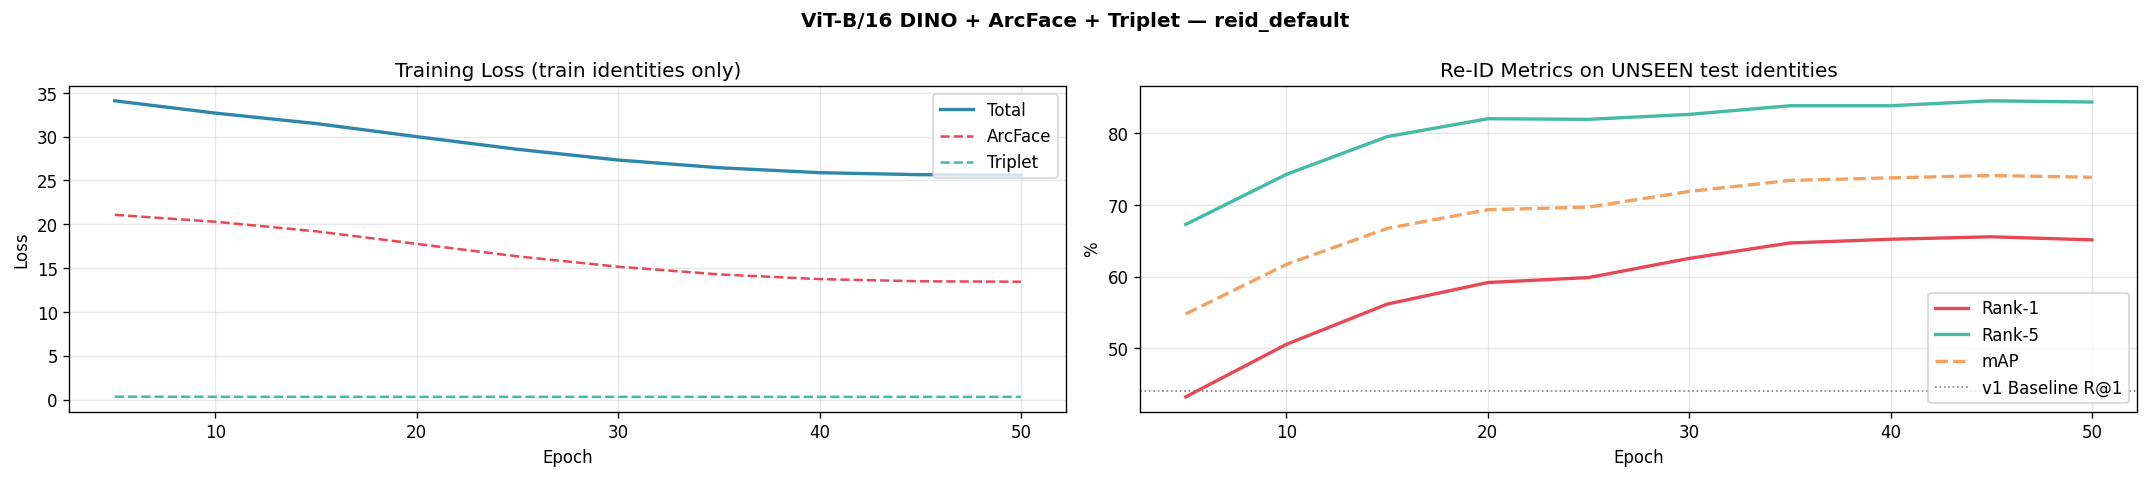
\includegraphics[width=\textwidth]{bab3/reid_default/training_curves.png}
    \caption{Kurva pelatihan konfigurasi acuan: (kiri) \textit{total loss} per \textit{epoch}; (kanan) \textit{Rank-1} dan mAP pada data validasi setiap 5 \textit{epoch}.}
    \label{fig:training_curves}
\end{figure}

% VERIFIKASI: cocokkan paragraf berikut dengan kurva aktual.
Ketiga kriteria tersebut terpenuhi pada konfigurasi acuan. \textit{Total loss} menurun secara monoton sepanjang 50 \textit{epoch} tanpa lonjakan, sehingga dapat disimpulkan bahwa kombinasi \textit{warmup} 5 \textit{epoch} dan \textit{gradient clipping} pada $G_{\max}=1{.}0$ memadai untuk menjaga kestabilan pelatihan. Metrik validasi meningkat tajam pada fase \textit{warmup}, kemudian melandai seiring aktifnya \textit{cosine decay} tanpa memperlihatkan penurunan pada \textit{epoch} akhir. Ketiadaan indikasi \textit{overfitting} pada anggaran $E=50$ ini konsisten dengan dua temuan yang diperoleh pada pengujian variasi, yaitu bahwa perpanjangan pelatihan hingga $E=100$ masih meningkatkan performa (Tabel~\ref{tab:var_epoch}) dan bahwa penambahan regularisasi justru menurunkan performa (Tabel~\ref{tab:var_dropout}). Dengan demikian dapat disimpulkan bahwa pada konfigurasi acuan model belum mencapai batas kapasitasnya, dan faktor pembatas utamanya adalah anggaran \textit{epoch}, bukan kekurangan regularisasi.

\subsection{Hasil Evaluasi Acuan}

Tabel~\ref{tab:baseline_results} menyajikan hasil evaluasi konfigurasi acuan pada dataset pengujian SeaTurtleIDHeads. Setiap metrik dilaporkan dua kali, yaitu menggunakan \textit{cosine similarity} murni (\textit{Cosine}) dan setelah \textit{k-reciprocal re-ranking} (\textit{+Re-rank}).

\begin{table}[H]
    \centering
    \caption{Hasil evaluasi konfigurasi acuan pada dataset pengujian SeaTurtleIDHeads}
    \label{tab:baseline_results}
    \renewcommand{\arraystretch}{1.35}
    \begin{tabular}{ l  c  c  c }
        \hline
        \textbf{Metrik} & \textbf{Cosine} & \textbf{+Re-rank} & \textbf{$\Delta$ (poin persentase)}                                                   \\
        \hline
        Rank-1  (\%)    & 77.4\%          & 78.3\%            & $+0{.}9$                                                                              \\
        Rank-5  (\%)    & 91.5\%          & 92.3\%            & $+0{.}8$                                                                              \\
        Rank-10 (\%)    & 95.9\%          & 95.1\%            & $-0{.}8$                                                                              \\
        mAP     (\%)    & 83.6\%          & 84.9\%            & $+1{.}3$                                                                              \\
        \hline
        \multicolumn{4}{l}{\footnotesize \textit{+Re-rank} = setelah k-reciprocal re-ranking ($k_1{=}20$, $k_2{=}6$, $\lambda_{\text{rr}}{=}0{.}3$).} \\
    \end{tabular}
\end{table}

\subsection{Analisis Hasil Acuan}

Berdasarkan hasil pada Tabel~\ref{tab:baseline_results}, beberapa observasi dapat dikemukakan.

\textbf{Pola antar-rank.} Akurasi meningkat seiring bertambahnya kedalaman peringkat yang ditoleransi, dengan pola perolehan yang menurun. Perpindahan dari \textit{Rank-1} ke \textit{Rank-5} memberikan peningkatan terbesar, yaitu dari 78.3\% menjadi 92.3\% atau sebesar 14.0 poin persentase, sedangkan perpindahan dari \textit{Rank-5} ke \textit{Rank-10} menghasilkan peningkatan yang jauh lebih kecil, yaitu dari 92.3\% menjadi 95.1\% atau sebesar 2.8 poin persentase. Pola tersebut memiliki implikasi praktis. Pada sekitar 14\% \textit{query}, identitas yang benar sesungguhnya telah berada di dalam lima kandidat teratas namun kalah tipis pada peringkat pertama, sehingga kegagalan model umumnya berupa kesalahan pengurutan pada peringkat teratas dan bukan kegagalan menemukan identitas yang benar. Sisa 4.9\% \textit{query} yang tetap gagal hingga \textit{Rank-10} merupakan kasus yang identitas benarnya memang tidak terjangkau, dan analisis kualitatif pada Subbab~\ref{subsec:kualitatif_id} menunjukkan bahwa kasus tersebut terkonsentrasi pada citra berkualitas rendah.

\textbf{Kontribusi re-ranking.} Efek \textit{k-reciprocal re-ranking} terhadap konfigurasi acuan bersifat positif namun tidak seragam. Pada \textit{Rank-1}, \textit{Rank-5}, dan mAP, re-ranking memberikan peningkatan masing-masing sebesar 0.9, 0.8, dan 1.3 poin persentase, yang menandakan bahwa struktur hubungan timbal balik antar tetangga dalam ruang \textit{embedding} berhasil dieksploitasi sebagai tahap pasca-proses tanpa biaya pelatihan tambahan. Sebaliknya, pada \textit{Rank-10} re-ranking sedikit menurunkan performa, yaitu dari 95.9\% menjadi 95.1\%. Pola tersebut wajar terjadi karena re-ranking mengoptimalkan konsistensi tetangga terdekat, sehingga paling menguntungkan pada peringkat teratas dan pada metrik agregat seperti mAP, sembari sesekali menggeser kandidat benar keluar dari rentang \textit{Rank-10} pada sebagian kecil \textit{query}. Perolehan bersihnya tetap positif, terutama pada mAP yang merupakan metrik paling representatif terhadap kualitas \textit{ranking} secara keseluruhan.

\subsection{Visualisasi t-SNE}

Gambar~\ref{fig:tsne} menampilkan visualisasi t-SNE dari vektor \textit{embedding} 20 identitas teratas pada data pengujian \textit{in-distribution}. Pengelompokan (\textit{clustering}) yang baik di ruang t-SNE, yaitu titik-titik dari identitas yang sama berdekatan dan terpisah dari identitas lain, mengkonfirmasi bahwa model berhasil membangun ruang \textit{embedding} yang diskriminatif.

\begin{figure}[H]
    \centering
    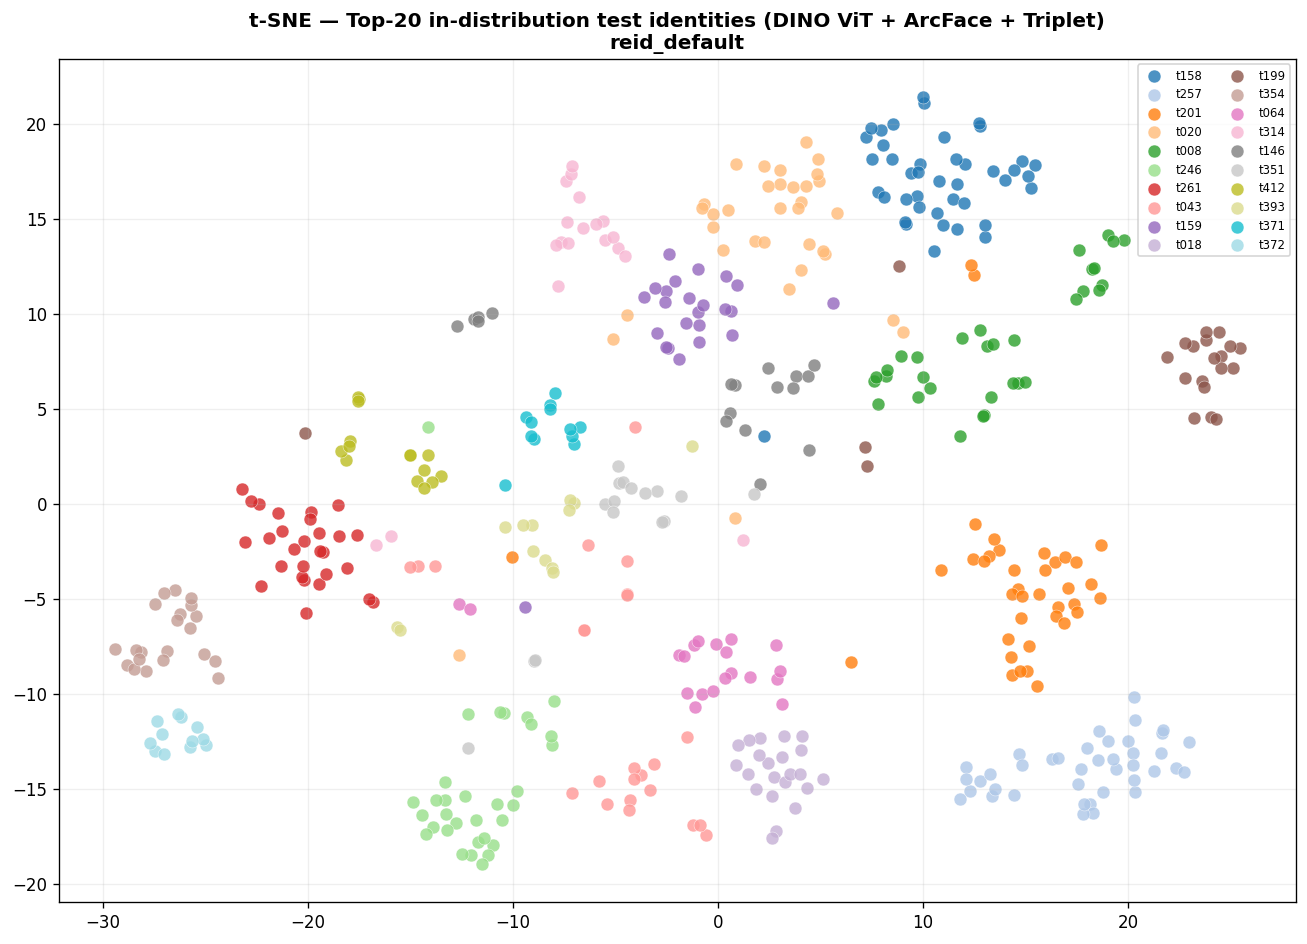
\includegraphics[width=0.85\textwidth]{bab4/tsne.png}
    \caption{Visualisasi t-SNE untuk 20 identitas penyu teratas pada data pengujian \textit{in-distribution}. Setiap warna mewakili satu identitas.}
    \label{fig:tsne}
\end{figure}

\subsection{Analisis Kualitatif Hasil Retrieval}
\label{subsec:kualitatif_id}

Gambar~\ref{fig:query_retrieval} menampilkan hasil \textit{retrieval} lima peringkat teratas untuk beberapa \textit{query} pada data pengujian \textit{in-distribution}, lengkap dengan skor \textit{cosine similarity} masing-masing kandidat.

\begin{figure}[H]
    \centering
    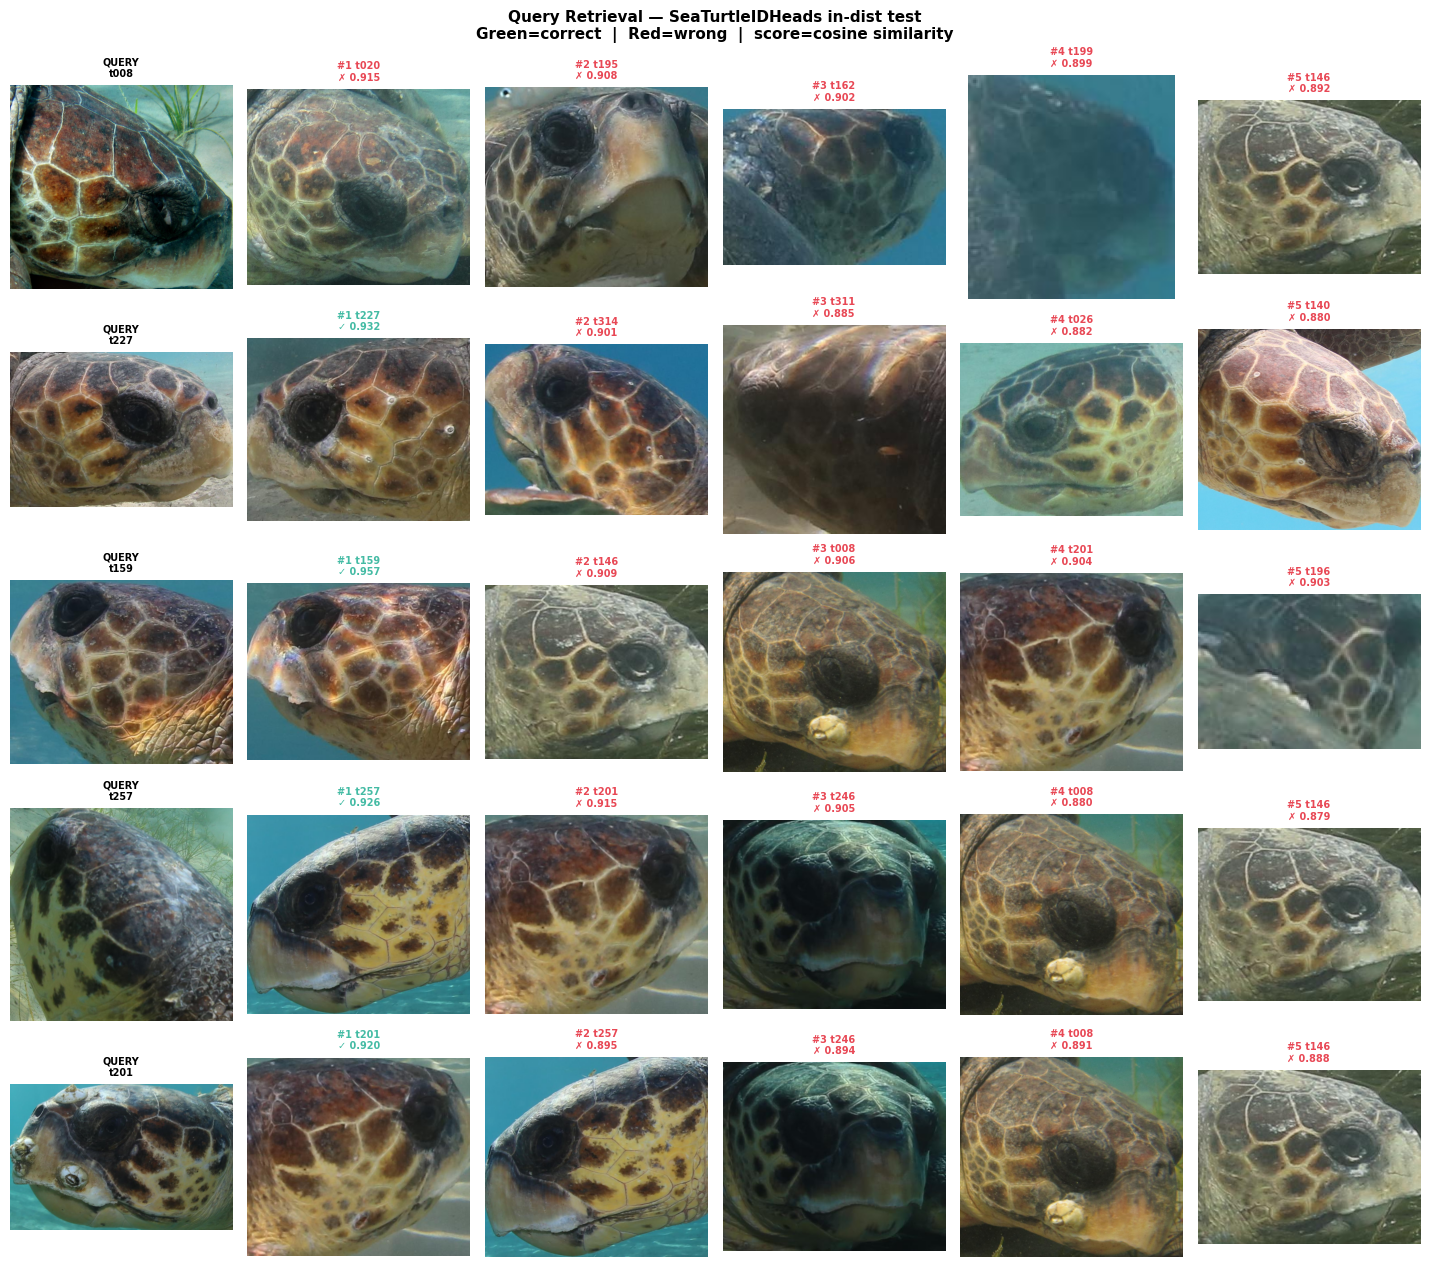
\includegraphics[width=\textwidth]{bab4/query_retrieval.png}
    \caption{Hasil \textit{retrieval} lima peringkat teratas pada data pengujian \textit{in-distribution} SeaTurtleIDHeads. Kolom pertama adalah citra \textit{query}, kolom berikutnya adalah kandidat galeri terurut menurun berdasarkan \textit{cosine similarity}. Hijau menandai identitas yang benar, merah menandai identitas yang salah.}
    \label{fig:query_retrieval}
\end{figure}

Dari Gambar~\ref{fig:query_retrieval} dapat dilihat bahwa pada \textit{query} yang berhasil (t227, t159, dan t257), kandidat peringkat-1 memperoleh skor yang jelas lebih tinggi daripada kandidat berikutnya, yaitu 0.932, 0.957, dan 0.926 terhadap kandidat kedua yang berada di sekitar 0.90. Hal ini menandakan bahwa model menemukan identitas yang benar dengan tingkat keyakinan yang terpisah dari kandidat pesaingnya.

Pengamatan pada kasus kegagalan menunjukkan bahwa kandidat yang keliru umumnya merupakan citra dengan pose kepala dan pencahayaan yang serupa dengan \textit{query}, atau citra yang buram dan berkontras rendah, misalnya kandidat \#3 dan \#4 pada baris t008. Hal ini mengindikasikan bahwa sisa kegagalan model terkonsentrasi pada citra berkualitas rendah, yaitu ketika pola sisik sebagai penanda identitas tidak lagi terbaca dengan jelas.

%% ============================================================
\section{Hasil Pengujian Variasi Parameter}
%% ============================================================

Bagian ini menyajikan hasil eksperimen variasi setiap parameter secara individual untuk menganalisis arah dan besar dampaknya terhadap performa. Metrik utama yang digunakan untuk perbandingan adalah \textit{Rank-1} dan mAP pada dataset pengujian SeaTurtleIDHeads dengan \textit{k-reciprocal re-ranking}. Untuk setiap parameter, fokus analisis diarahkan pada arah perubahan performa relatif terhadap acuan dan pada sensitivitas sistem terhadap parameter tersebut.

\subsection{Variasi Parameter Dataset}

\subsubsection{Ukuran Citra (\textit{img\_size})}

\begin{table}[H]
    \centering
    \caption{Pengaruh ukuran citra terhadap performa (+Re-rank)}
    \label{tab:var_imgsize}
    \renewcommand{\arraystretch}{1.25}
    \begin{tabular}{ccccc}
        \hline
        $\mathit{img\_size}$ & \textbf{Rank-1 (\%)} & \textbf{Rank-5 (\%)} & \textbf{Rank-10 (\%)} & \textbf{mAP (\%)} \\
        \hline
        224                  & 73.3\%               & 91.5\%               & 94.9\%                & 81.9\%            \\
        \textbf{256}         & 78.3\%               & 92.3\%               & 95.1\%                & 84.9\%            \\
        320                  & 76.1\%               & 92.5\%               & 96.0\%                & 84.9\%            \\
        \hline
    \end{tabular}
\end{table}

Berdasarkan hasil pengujian tersebut, pengaruh resolusi citra terhadap performa tidak bersifat monoton. Peningkatan resolusi dari 224 ke 256 (acuan) meningkatkan seluruh metrik secara jelas, dengan Rank-1 naik sebesar 5.0 poin persentase. Namun peningkatan lebih lanjut ke 320 tidak lagi memberikan perbaikan yang konsisten, yaitu Rank-1 justru menurun menjadi 76.1\% atau di bawah acuan 78.3\%, meskipun Rank-5, Rank-10, dan mAP sedikit lebih tinggi atau setara. Dengan mempertimbangkan bahwa resolusi yang lebih tinggi menuntut kebutuhan komputasi yang lebih besar tanpa keunggulan yang meyakinkan pada Rank-1, resolusi 256 dipertahankan sebagai nilai acuan yang memberikan keseimbangan terbaik antara performa dan biaya komputasi.

\subsubsection{Jumlah Citra Galeri per Identitas (\textit{n\_gallery})}

\begin{table}[H]
    \centering
    \caption{Pengaruh jumlah citra galeri per identitas terhadap performa (+Re-rank)}
    \label{tab:var_ngallery}
    \renewcommand{\arraystretch}{1.25}
    \begin{tabular}{ccccc}
        \hline
        $N_G$      & \textbf{Rank-1 (\%)} & \textbf{Rank-5 (\%)} & \textbf{Rank-10 (\%)} & \textbf{mAP (\%)} \\
        \hline
        1          & 58.2\%               & 83.9\%               & 92.8\%                & 69.3\%            \\
        \textbf{3} & 78.3\%               & 92.3\%               & 95.1\%                & 84.9\%            \\
        5          & 69.5\%               & 90.4\%               & 93.6\%                & 78.3\%            \\
        \hline
    \end{tabular}
\end{table}

Berdasarkan data tersebut, $N_G=3$ menghasilkan performa tertinggi, diikuti oleh $N_G=5$ dan $N_G=1$. Secara teoretis, $N_G=5$ diharapkan menghasilkan prototipe yang paling stabil dan karenanya performa tertinggi. Penurunan yang teramati berasal dari efek samping konstruksi \textit{split}, yaitu bertambahnya $N_G$ menaikkan ambang minimum citra per identitas sehingga jumlah identitas yang memenuhi syarat berkurang, sekaligus mengurangi jumlah citra \textit{query} yang tersisa. Perlu ditegaskan bahwa karena komposisi \textit{query} dan galeri berubah antar-nilai $N_G$, ketiga baris pada tabel tersebut tidak dievaluasi pada himpunan \textit{query} yang identik. Perbandingan antar-baris karenanya bersifat indikatif terhadap konfigurasi sistem secara keseluruhan, dan bukan merupakan perbandingan performa model murni pada tugas yang sama.

\subsection{Variasi Parameter Arsitektur}

\subsubsection{Backbone}

\begin{table}[H]
    \centering
    \caption{Pengaruh pemilihan backbone terhadap performa (+Re-rank)}
    \label{tab:var_backbone}
    \renewcommand{\arraystretch}{1.25}
    \begin{tabular}{lcccc}
        \hline
        \textbf{Backbone} & \textbf{Rank-1 (\%)} & \textbf{Rank-5 (\%)} & \textbf{Rank-10 (\%)} & \textbf{mAP (\%)} \\
        \hline
        ViT-S/16          & 61.4\%               & 82.1\%               & 91.0\%                & 70.3\%            \\
        \textbf{ViT-B/16} & 78.3\%               & 92.3\%               & 95.1\%                & 84.9\%            \\
        ViT-L/16          & 80.4\%               & 94.4\%               & 96.2\%                & 86.6\%            \\
        \hline
    \end{tabular}
\end{table}

Performa meningkat secara konsisten seiring bertambahnya ukuran \textit{backbone}, dari ViT-S/16 hingga ViT-L/16, pada seluruh metrik yang diukur. Peningkatan dari ViT-S/16 ke ViT-B/16 tergolong besar, yaitu Rank-1 naik sebesar 16.9 poin persentase, sedangkan peningkatan dari ViT-B/16 ke ViT-L/16 jauh lebih moderat, yaitu Rank-1 naik sebesar 2.1 poin persentase. Hal ini menunjukkan bahwa kapasitas representasi \textit{backbone} yang lebih besar membantu membedakan identitas penyu secara lebih baik, meskipun disertai \textit{diminishing return} yang tajam serta konsekuensi kebutuhan komputasi dan memori yang jauh lebih besar pada ViT-L/16.

\subsubsection{Dimensi Embedding (\textit{embed\_dim})}

\begin{table}[H]
    \centering
    \caption{Pengaruh dimensi embedding terhadap performa (+Re-rank)}
    \label{tab:var_embeddim}
    \renewcommand{\arraystretch}{1.25}
    \begin{tabular}{ccccc}
        \hline
        $d_e$        & \textbf{Rank-1 (\%)} & \textbf{Rank-5 (\%)} & \textbf{Rank-10 (\%)} & \textbf{mAP (\%)} \\
        \hline
        128          & 76.5\%               & 92.1\%               & 95.3\%                & 84.0\%            \\
        \textbf{256} & 78.3\%               & 92.3\%               & 95.1\%                & 84.9\%            \\
        512          & 76.6\%               & 92.1\%               & 94.7\%                & 83.9\%            \\
        \hline
    \end{tabular}
\end{table}

Ketiga nilai dimensi \textit{embedding} yang diuji menghasilkan performa yang berdekatan, dengan selisih Rank-1 tidak lebih dari 1.8 poin persentase dan selisih mAP tidak lebih dari 1.0 poin persentase. Hal ini menandakan bahwa sistem relatif robust terhadap parameter tersebut. Meski demikian, terdapat pola \textit{inverted-U}, yaitu $d_e=256$ memberikan performa terbaik pada Rank-1 (78.3\%) dan mAP (84.9\%), sementara dimensi yang lebih kecil ($d_e=128$) maupun yang lebih besar ($d_e=512$) sama-sama menurunkan performa hingga ke tingkat yang nyaris identik (Rank-1 76.5\% berbanding 76.6\%). Secara teoretis kedua penurunan tersebut berasal dari mekanisme yang berlawanan. Dimensi 128 terlalu ringkas untuk memisahkan identitas penyu yang bersifat \textit{fine-grained} sehingga kehilangan daya ekspresif, sedangkan dimensi 512 menambah kapasitas berlebih yang rentan \textit{overfitting} pada dataset berskala terbatas tanpa memberikan informasi diskriminatif tambahan. Perlu dicatat bahwa selisih sebesar itu berada pada orde beberapa \textit{query} saja, sehingga pola \textit{inverted-U} tersebut sebaiknya dibaca sebagai indikasi ketidakpekaan sistem terhadap $d_e$ dan bukan sebagai bukti kuat adanya titik optimum. Efeknya pun terkonsentrasi pada Rank-1 dan mAP, sedangkan Rank-5 dan Rank-10 hampir tidak berubah antar-nilai, dengan Rank-5 berada pada rentang 92.1\% hingga 92.3\%. Dengan demikian $d_e=256$ dipertahankan sebagai acuan.

\subsubsection{Dropout}

\begin{table}[H]
    \centering
    \caption{Pengaruh dropout terhadap performa (+Re-rank)}
    \label{tab:var_dropout}
    \renewcommand{\arraystretch}{1.25}
    \begin{tabular}{ccccc}
        \hline
        $p_{\text{drop}}$ & \textbf{Rank-1 (\%)} & \textbf{Rank-5 (\%)} & \textbf{Rank-10 (\%)} & \textbf{mAP (\%)} \\
        \hline
        0{.}0            & 81.0\%               & 91.7\%               & 94.9\%                & 86.0\%             \\
        \textbf{0{.}1}    & 78.3\%               & 92.3\%               & 95.1\%                & 84.9\%            \\
        0{.}3             & 73.1\%               & 90.8\%               & 95.1\%                & 81.2\%            \\
        \hline
    \end{tabular}
\end{table}

Berbeda dengan ekspektasi umum bahwa \textit{dropout} membantu regularisasi, performa pada pengujian ini justru menurun secara monoton seiring bertambahnya $p_{\text{drop}}$. Nilai $p_{\text{drop}}=0{.}0$ memberikan performa terbaik pada Rank-1 (81.0\%) dan mAP (86.0\%), keduanya lebih tinggi daripada acuan $p_{\text{drop}}=0{.}1$, sedangkan $p_{\text{drop}}=0{.}3$ menurunkan Rank-1 secara tajam hingga 73.1\%. Pola tersebut mengindikasikan bahwa model tidak berada pada rezim \textit{overfitting} yang membutuhkan regularisasi \textit{dropout}; sebaliknya, penonaktifan neuron secara acak justru membuang kapasitas representasi yang masih berguna. Temuan ini konsisten dengan hasil pada bobot Triplet Loss (Tabel~\ref{tab:var_tripletweight}) dan \textit{weight decay} (Tabel~\ref{tab:var_wd}), yang sama-sama menunjukkan bahwa regularisasi tambahan cenderung tidak menguntungkan pada konfigurasi ini, kemungkinan besar karena fitur \textit{self-supervised} DINOv3 yang telah terlatih sudah berperan sebagai regularisasi implisit yang kuat. Terdapat satu catatan penimbang, yaitu pada $p_{\text{drop}}=0{.}0$ nilai Rank-5 dan Rank-10 sedikit lebih rendah dibandingkan acuan, dengan Rank-5 sebesar 91.7\% berbanding 92.3\%, sehingga keunggulan penonaktifan \textit{dropout} paling terasa pada presisi teratas (Rank-1) dan pada metrik agregat (mAP). Meskipun data mendukung $p_{\text{drop}}=0{.}0$, penonaktifan \textit{dropout} sepenuhnya berpotensi meningkatkan risiko \textit{overfitting} pada skenario data yang lebih sempit, sehingga nilai tersebut menjadi kandidat kuat namun tetap perlu diverifikasi bersama parameter lain.

\subsection{Variasi Parameter Loss}

\subsubsection{Skala ArcFace (\textit{arcface\_scale})}

\begin{table}[H]
    \centering
    \caption{Pengaruh skala ArcFace terhadap performa (+Re-rank)}
    \label{tab:var_arcscale}
    \renewcommand{\arraystretch}{1.25}
    \begin{tabular}{ccccc}
        \hline
        $s_a$           & \textbf{Rank-1 (\%)} & \textbf{Rank-5 (\%)} & \textbf{Rank-10 (\%)} & \textbf{mAP (\%)} \\
        \hline
        16{.}0          & 72.9\%               & 91.9\%               & 94.9\%                & 81.7\%            \\
        \textbf{32{.}0} & 78.3\%               & 92.3\%               & 95.1\%                & 84.9\%            \\
        64{.}0          & 76.6\%               & 91.1\%               & 94.7\%                & 83.3\%            \\
        \hline
    \end{tabular}
\end{table}

Pengaruh skala ArcFace terhadap performa membentuk pola \textit{inverted-U} dengan puncak pada nilai acuan $s_a=32{.}0$. Penurunan skala ke 16.0 menurunkan seluruh metrik, khususnya Rank-1 yang turun sebesar 5.4 poin persentase dan mAP sebesar 3.2 poin persentase. Skala yang terlalu kecil membuat distribusi \textit{softmax} atas logit sudut menjadi terlalu landai, sehingga separasi antar-kelas melemah dan gradien tidak cukup menekan pemisahan identitas yang mirip. Sebaliknya, peningkatan skala ke 64.0 juga menurunkan performa dibandingkan acuan, yaitu Rank-1 sebesar 76.6\% dan mAP sebesar 83.3\%, meskipun tetap lebih baik daripada skala 16.0. Skala yang terlalu besar membuat logit menjadi terlalu tajam dan mudah jenuh sehingga gradien menjadi runcing dan optimisasi kurang stabil, dan efek tersebut diperberat oleh jumlah kelas yang sedikit pada dataset ini. Hasil tersebut mengonfirmasi justifikasi pemilihan acuan, yaitu bahwa nilai 64 yang lazim pada dataset wajah berskala besar memang kurang sesuai untuk jumlah identitas yang jauh lebih kecil pada penelitian ini, dan skala moderat 32.0 memberikan ketajaman distribusi sudut yang paling seimbang.

\subsubsection{Margin ArcFace (\textit{arcface\_margin})}

\begin{table}[H]
    \centering
    \caption{Pengaruh margin ArcFace terhadap performa (+Re-rank)}
    \label{tab:var_arcmargin}
    \renewcommand{\arraystretch}{1.25}
    \begin{tabular}{ccccc}
        \hline
        $m_a$          & \textbf{Rank-1 (\%)} & \textbf{Rank-5 (\%)} & \textbf{Rank-10 (\%)} & \textbf{mAP (\%)} \\
        \hline
        0{.}3         & 77.2\%               & 91.7\%               & 94.7\%                & 84.1\%             \\
        \textbf{0{.}5} & 78.3\%               & 92.3\%               & 95.1\%                & 84.9\%            \\
        1{.}0          & 80.0\%               & 92.1\%               & 95.3\%                & 85.8\%            \\
        2{.}0          & 76.5\%               & 91.1\%               & 94.4\%                & 83.7\%            \\
        \hline
    \end{tabular}
\end{table}

Performa terbaik justru dicapai pada $m_a=1{.}0$, yaitu sedikit lebih tinggi dibandingkan nilai acuan $m_a=0{.}5$, dengan Rank-1 sebesar 80.0\% berbanding 78.3\% dan mAP sebesar 85.8\% berbanding 84.9\%. Namun ketika margin diperbesar lebih lanjut menjadi $m_a=2{.}0$, performa menurun hingga di bawah nilai acuan. Pola tersebut menunjukkan adanya titik optimal margin, yaitu margin yang cukup besar untuk memberikan separasi antar-kelas yang kuat namun tidak terlalu besar sehingga menyulitkan konvergensi optimisasi ArcFace.

\subsubsection{Margin Triplet (\textit{triplet\_margin})}

\begin{table}[H]
    \centering
    \caption{Pengaruh margin Triplet terhadap performa (+Re-rank)}
    \label{tab:var_tripletmargin}
    \renewcommand{\arraystretch}{1.25}
    \begin{tabular}{ccccc}
        \hline
        $m_t$          & \textbf{Rank-1 (\%)} & \textbf{Rank-5 (\%)} & \textbf{Rank-10 (\%)} & \textbf{mAP (\%)} \\
        \hline
        0{.}1         & 76.5\%               & 91.5\%               & 95.1\%                & 83.6\%             \\
        \textbf{0{.}3} & 78.3\%               & 92.3\%               & 95.1\%                & 84.9\%            \\
        0{.}5          & 78.0\%               & 92.3\%               & 95.5\%                & 84.6\%            \\
        \hline
    \end{tabular}
\end{table}

Perbedaan performa antar nilai margin Triplet relatif kecil dibandingkan parameter lain, yang mengindikasikan bahwa sistem tidak terlalu sensitif terhadap parameter tersebut. Margin yang lebih besar ($m_t=0{.}5$) memberikan Rank-10 yang sedikit lebih baik, sementara margin yang lebih kecil ($m_t=0{.}1$) sedikit menurunkan performa Rank-1 dan mAP, namun secara keseluruhan selisihnya tidak lebih dari 1.8 poin persentase pada setiap metrik. Ketidakpekaan tersebut konsisten dengan temuan pada bobot Triplet (Tabel~\ref{tab:var_tripletweight}), yaitu apabila kontribusi Triplet Loss terhadap performa memang kecil atau bahkan negatif, maka wajar apabila penyetelan marginnya juga berdampak minim.

\subsubsection{Bobot Triplet (\textit{triplet\_weight})}

\begin{table}[H]
    \centering
    \caption{Pengaruh bobot Triplet Loss terhadap performa (+Re-rank)}
    \label{tab:var_tripletweight}
    \renewcommand{\arraystretch}{1.25}
    \begin{tabular}{ccccc}
        \hline
        $\lambda_t$     & \textbf{Rank-1 (\%)} & \textbf{Rank-5 (\%)} & \textbf{Rank-10 (\%)} & \textbf{mAP (\%)} \\
        \hline
        0{.}00          & 83.4\%               & 94.5\%               & 97.6\%                & 88.4\%            \\
        0{.}20          & 80.6\%               & 92.1\%               & 96.0\%                & 86.6\%            \\
        \textbf{0{.}50} & 78.3\%               & 92.3\%               & 95.1\%                & 84.9\%            \\
        0{.}80          & 77.6\%               & 91.9\%               & 95.3\%                & 84.1\%            \\
        \hline
    \end{tabular}
\end{table}

Performa tertinggi justru dicapai ketika Triplet Loss tidak diikutsertakan sama sekali ($\lambda_t=0{.}0$), yaitu dengan Rank-1 sebesar 83.4\% dan mAP sebesar 88.4\%, keduanya lebih tinggi dibandingkan konfigurasi acuan. Performa menurun secara monoton pada seluruh metrik seiring bertambahnya bobot Triplet Loss. Hal ini mengindikasikan bahwa pada konfigurasi dan skala dataset ini, ArcFace Loss saja sudah cukup diskriminatif, sementara penambahan Triplet Loss justru mengganggu proses optimisasi. Temuan tersebut memiliki implikasi lanjutan, yaitu karena $\lambda_t=0{.}0$ menonaktifkan Triplet Loss sepenuhnya, komposisi \textit{PK-sampling} ($P$ dan $K$) kehilangan justifikasi utamanya sebagai penjamin ketersediaan pasangan positif untuk penambangan \textit{triplet}. Hal ini menjelaskan mengapa $K=2$ justru mengungguli $K=4$ pada Tabel~\ref{tab:var_batch}.

\subsection{Variasi Parameter Pelatihan}

\subsubsection{Komposisi Batch: Identitas per Batch ($P$) dan Citra per Identitas ($K$)}

\begin{table}[H]
    \centering
    \caption{Pengaruh komposisi batch terhadap performa (+Re-rank)}
    \label{tab:var_batch}
    \renewcommand{\arraystretch}{1.25}
    \begin{tabular}{cccccc}
        \hline
        $P$         & $K$        & \textbf{Batch Size} & \textbf{Rank-1 (\%)} & \textbf{Rank-5 (\%)} & \textbf{mAP (\%)} \\
        \hline
        8           & \textbf{4} & 32                  & 79.1\%               & 92.1\%               & 85.5\%            \\
        \textbf{16} & \textbf{4} & \textbf{64}         & 78.3\%               & 92.3\%               & 84.9\%            \\
        32          & \textbf{4} & 128                 & 68.5\%               & 88.7\%               & 78.2\%            \\
        \textbf{16} & 2          & 32                  & 79.1\%               & 95.3\%               & 86.3\%            \\
        \textbf{16} & 8          & 128                 & 71.9\%               & 88.9\%               & 80.1\%            \\
        \hline
        % VERIFIKASI: kolom Rank-10 belum dilengkapi.
    \end{tabular}
\end{table}

Pola pada tabel tersebut paling jelas dibaca melalui \textit{batch size} efektif, dan bukan melalui $P$ atau $K$ secara terpisah. Kedua konfigurasi dengan \textit{batch size} 32, yaitu $P=8, K=4$ dan $P=16, K=2$, memberikan Rank-1 yang identik sebesar 79.1\% dan keduanya sedikit di atas acuan. Sebaliknya kedua konfigurasi dengan \textit{batch size} 128, yaitu $P=32, K=4$ dan $P=16, K=8$, sama-sama mengalami penurunan tajam dengan Rank-1 sebesar 68.5\% dan 71.9\%. Kesamaan tersebut menunjukkan bahwa faktor penentunya bukanlah komposisi identitas per \textit{batch}, melainkan jumlah iterasi pembaruan bobot yang tersedia. Pada anggaran $E=50$ yang tetap, \textit{batch size} 128 memangkas jumlah iterasi per \textit{epoch} menjadi seperempat dari \textit{batch size} 32, sehingga model belum sempat mencapai konvergensi. Interpretasi tersebut diperkuat oleh Tabel~\ref{tab:var_epoch} yang menunjukkan bahwa pada acuan pun model masih kekurangan iterasi. Dengan demikian penurunan pada $P=32$ dan $K=8$ sebaiknya tidak dibaca sebagai kerugian akibat berkurangnya keberagaman identitas per iterasi, melainkan sebagai gejala kekurangan iterasi yang sama.

\subsubsection{Jumlah Epoch}

\begin{table}[H]
    \centering
    \caption{Pengaruh jumlah epoch terhadap performa (+Re-rank)}
    \label{tab:var_epoch}
    \renewcommand{\arraystretch}{1.25}
    \begin{tabular}{ccccc}
        \hline
        $E$         & \textbf{Rank-1 (\%)} & \textbf{Rank-5 (\%)} & \textbf{Rank-10 (\%)} & \textbf{mAP (\%)} \\
        \hline
        30          & 69.7\%               & 89.6\%               & 93.6\%                & 79.4\%            \\
        \textbf{50} & 78.3\%               & 92.3\%               & 95.1\%                & 84.9\%            \\
        100         & 84.4\%               & 93.2\%               & 96.0\%                & 88.4\%            \\
        \hline
        \multicolumn{5}{l}{\footnotesize \textit{Warmup epoch} dijaga tetap pada $W$=5.}                      \\
    \end{tabular}
\end{table}

Performa meningkat secara konsisten dan substansial seiring bertambahnya jumlah \textit{epoch} pelatihan, yaitu dari $E=30$ hingga $E=100$ Rank-1 naik dari 69.7\% menjadi 84.4\% dan mAP naik dari 79.4\% menjadi 88.4\%, tanpa tanda saturasi yang jelas pada rentang yang diuji. Hal ini mengindikasikan bahwa model masih dapat terus belajar dengan pelatihan yang lebih panjang, meskipun disertai konsekuensi waktu komputasi yang lebih besar. Konsekuensi metodologisnya perlu dicatat, yaitu karena acuan $E=50$ berada pada rezim \textit{under-training}, sebagian parameter lain kemungkinan dinilai pada titik operasi yang belum konvergen. Hal tersebut menjadi salah satu batasan pendekatan OFAT pada penelitian ini. Jumlah \textit{epoch} termasuk salah satu parameter paling berdampak pada pengujian ini, dan $E=100$ menjadi salah satu komponen yang kemudian diadopsi pada konfigurasi kombinasi.

\subsubsection{Warmup Epoch}

\begin{table}[H]
    \centering
    \caption{Pengaruh warmup epoch terhadap performa (+Re-rank)}
    \label{tab:var_warmup}
    \renewcommand{\arraystretch}{1.25}
    \begin{tabular}{ccccc}
        \hline
        $W$        & \textbf{Rank-1 (\%)} & \textbf{Rank-5 (\%)} & \textbf{Rank-10 (\%)} & \textbf{mAP (\%)} \\
        \hline
        3          & 81.0\%               & 91.3\%               & 94.9\%                & 86.1\%            \\
        \textbf{5} & 78.3\%               & 92.3\%               & 95.1\%                & 84.9\%            \\
        10         & 80.0\%               & 91.3\%               & 95.7\%                & 85.4\%            \\
        \hline
        \multicolumn{5}{l}{\footnotesize Jumlah \textit{epoch} dijaga tetap pada $E$=50.}                    \\
    \end{tabular}
\end{table}

Pada variasi \textit{warmup epoch} dengan $E=50$ yang dijaga tetap, baik $W=3$ maupun $W=10$ memberikan Rank-1 yang sedikit lebih tinggi dibandingkan acuan $W=5$, yaitu sebesar 81.0\% dan 80.0\% berbanding 78.3\%, dengan $W=3$ memberikan mAP tertinggi sebesar 86.1\%. Pola tersebut tidak monoton karena acuan justru menjadi titik terendah di antara ketiga nilai, sehingga tidak dapat ditafsirkan sebagai hubungan sebab-akibat yang bersih antara panjang \textit{warmup} dan performa. Interpretasi yang lebih hati-hati adalah bahwa selisih antar-nilai tergolong kecil, yaitu Rank-1 berada dalam rentang 78.3\% hingga 81.0\%, sehingga sistem relatif tidak sensitif terhadap panjang \textit{warmup} pada rentang yang diuji. Kecenderungan $W=3$ yang sedikit unggul tetap konsisten dengan penjelasan bahwa pada anggaran \textit{epoch} yang tetap, porsi \textit{epoch} yang dihabiskan pada laju belajar rendah menyisakan lebih sedikit iterasi pada laju belajar penuh, sejalan dengan indikasi \textit{under-training} pada Tabel~\ref{tab:var_epoch}.

\subsubsection{Gradient Clipping (\textit{grad\_clip})}

\begin{table}[H]
    \centering
    \caption{Pengaruh gradient clipping terhadap performa (+Re-rank)}
    \label{tab:var_gradclip}
    \renewcommand{\arraystretch}{1.25}
    \begin{tabular}{ccccc}
        \hline
        $G_{\max}$     & \textbf{Rank-1 (\%)} & \textbf{Rank-5 (\%)} & \textbf{Rank-10 (\%)} & \textbf{mAP (\%)} \\
        \hline
        0{.}5         & 76.6\%               & 91.9\%               & 95.7\%                & 83.9\%             \\
        \textbf{1{.}0} & 78.3\%               & 92.3\%               & 95.1\%                & 84.9\%            \\
        5{.}0          & 78.3\%               & 91.7\%               & 94.9\%                & 84.2\%            \\
        \hline
    \end{tabular}
\end{table}

Perbedaan performa antar nilai \textit{gradient clipping} relatif kecil, dengan rentang Rank-1 hanya sebesar 1.7 poin persentase. Nilai acuan $G_{\max}=1{.}0$ dan nilai $G_{\max}=5{.}0$ menghasilkan Rank-1 yang identik sebesar 78.3\%, dengan nilai acuan sedikit unggul pada metrik lainnya. Perlu dicatat bahwa kesamaan antara $G_{\max}=1{.}0$ dan $G_{\max}=5{.}0$ kemungkinan besar bukan merupakan kebetulan, melainkan disebabkan norma gradien aktual selama pelatihan jarang melampaui 5.0 sehingga ambang tersebut praktis tidak pernah aktif. Dengan demikian dampak parameter ini pada rentang nilai yang diuji memang kecil, dan pembatasan gradien di sekitar 1.0 sudah memadai untuk menjaga kestabilan tanpa memperlambat pembelajaran.

\subsubsection{Patience Early Stopping}

\begin{table}[H]
    \centering
    \caption{Pengaruh patience early stopping terhadap performa (+Re-rank)}
    \label{tab:var_patience}
    \renewcommand{\arraystretch}{1.25}
    \begin{tabular}{ccccc}
        \hline
        $P_{\text{stop}}$ & \textbf{Rank-1 (\%)} & \textbf{Rank-5 (\%)} & \textbf{Rank-10 (\%)} & \textbf{mAP (\%)} \\
        \hline
        5                 & 77.6\%               & 91.5\%               & 94.9\%                & 84.5\%            \\
        \textbf{10}       & 78.3\%               & 92.3\%               & 95.1\%                & 84.9\%            \\
        20                & 78.5\%               & 91.1\%               & 95.1\%                & 84.9\%            \\
        40                & 78.3\%               & 91.7\%               & 95.5\%                & 84.9\%            \\
        \hline
    \end{tabular}
\end{table}

Nilai \textit{patience} tidak memberikan pengaruh berarti terhadap performa akhir, dengan seluruh nilai yang diuji menghasilkan Rank-1 pada rentang 77.6\% hingga 78.5\% dan mAP pada rentang 84.5\% hingga 84.9\%. Ketiadaan pengaruh tersebut bersifat struktural dan bukan sekadar indikasi model yang robust. Dengan interval evaluasi setiap 5 \textit{epoch} dan anggaran $E=50$, nilai $P_{\text{stop}}=10$ interval setara dengan 50 \textit{epoch}, yaitu persis seluruh durasi pelatihan, sehingga \textit{early stopping} pada konfigurasi acuan tidak mungkin terpicu. Hal yang sama berlaku untuk $P_{\text{stop}}=20$ dan $P_{\text{stop}}=40$ yang bahkan melampaui total \textit{epoch}. Ketiga nilai tersebut secara efektif menonaktifkan \textit{early stopping}, sehingga kesamaan performanya sudah dapat diperkirakan tanpa eksperimen. Hanya $P_{\text{stop}}=5$, yang setara dengan 25 \textit{epoch} tanpa perbaikan, berpeluang aktif, dan nilai tersebut memang satu-satunya yang sedikit berbeda. Kesimpulan yang dapat ditarik karenanya bukan bahwa \textit{patience} tidak berpengaruh, melainkan bahwa pada anggaran \textit{epoch} ini \textit{patience} bukan merupakan parameter yang mengikat.

\subsection{Variasi Parameter Optimizer}

\subsubsection{Weight Decay}

\begin{table}[H]
    \centering
    \caption{Pengaruh weight decay terhadap performa (+Re-rank)}
    \label{tab:var_wd}
    \renewcommand{\arraystretch}{1.25}
    \begin{tabular}{ccccc}
        \hline
        $\lambda_w$        & \textbf{Rank-1 (\%)} & \textbf{Rank-5 (\%)} & \textbf{Rank-10 (\%)} & \textbf{mAP (\%)} \\
        \hline
        $10^{-5}$          & 79.1\%               & 92.1\%               & 94.9\%                & 85.2\%            \\
        $\mathbf{10^{-4}}$ & 78.3\%               & 92.3\%               & 95.1\%                & 84.9\%            \\
        $10^{-3}$          & 78.5\%               & 91.3\%               & 95.3\%                & 84.9\%            \\
        \hline
    \end{tabular}
\end{table}

Seluruh nilai \textit{weight decay} yang diuji menghasilkan performa yang berdekatan, yaitu Rank-1 pada rentang 78.3\% hingga 79.1\% dan mAP pada rentang 84.9\% hingga 85.2\%, dengan $\lambda_w=10^{-5}$ memberikan performa yang sedikit lebih baik dibandingkan nilai acuan. \textit{Weight decay} karenanya merupakan parameter yang paling tidak sensitif pada pengujian ini. Arah perubahannya, meskipun kecil, konsisten dengan temuan pada \textit{dropout} (Tabel~\ref{tab:var_dropout}) dan bobot Triplet (Tabel~\ref{tab:var_tripletweight}), yaitu regularisasi eksplisit yang lebih longgar cenderung sedikit menguntungkan. Ketiga hasil tersebut mengarah pada penjelasan yang sama, yaitu bahwa model tidak berada pada rezim \textit{overfitting} sehingga tidak membutuhkan regularisasi tambahan, kemungkinan besar karena \textit{fine-tuning} konservatif atas fitur \textit{self-supervised} DINOv3 dan augmentasi data sudah memberikan efek regularisasi implisit yang memadai.

\subsubsection{Base Learning Rate}

\begin{table}[H]
    \centering
    \caption{Pengaruh base learning rate terhadap performa (+Re-rank)}
    \label{tab:var_baselr}
    \renewcommand{\arraystretch}{1.25}
    \begin{tabular}{ccccc}
        \hline
        $\eta_{\text{base}}$ & \textbf{Rank-1 (\%)} & \textbf{Rank-5 (\%)} & \textbf{Rank-10 (\%)} & \textbf{mAP (\%)} \\
        \hline
        $10^{-4}$            & 56.3\%               & 84.4\%               & 90.6\%                & 68.6\%            \\
        $\mathbf{10^{-3}}$   & 78.3\%               & 92.3\%               & 95.1\%                & 84.9\%            \\
        $10^{-2}$            & 53.1\%               & 87.4\%               & 92.3\%                & 67.3\%            \\
        \hline
        \multicolumn{5}{l}{\footnotesize \textit{Backbone base LR} dijaga tetap pada $\eta_{\text{bb}}=10^{-5}$.}      \\
    \end{tabular}
\end{table}

\textit{Base learning rate} merupakan parameter paling sensitif pada sistem ini, dengan rentang Rank-1 mencapai 25.2 poin persentase. Dengan \textit{backbone base LR} dijaga tetap pada $10^{-5}$, baik peningkatan $\eta_{\text{base}}$ ke $10^{-2}$ maupun penurunannya ke $10^{-4}$ menyebabkan penurunan performa yang drastis, yaitu Rank-1 masing-masing turun menjadi 53.1\% dan 56.3\% atau keduanya di bawah 57\%. Hal ini menunjukkan bahwa proses optimisasi \textit{head} klasifikasi/\textit{metric learning}, yang diinisialisasi secara acak, sangat bergantung pada laju belajar yang tepat. Laju belajar yang terlalu tinggi membuat optimisasi tidak stabil dan gagal konvergen, sedangkan laju belajar yang terlalu rendah membuat \textit{head} tidak sempat belajar dalam anggaran \textit{epoch} yang tersedia. Nilai acuan $10^{-3}$ berada tepat pada titik operasi yang sempit namun optimal. Perlu dicatat bahwa karena hanya tiga nilai berjarak satu dekade yang diuji, hasil ini tidak menutup kemungkinan adanya nilai yang lebih baik di antara $10^{-3}$ dan tetangganya.

\subsubsection{Backbone Base Learning Rate}

\begin{table}[H]
    \centering
    \caption{Pengaruh backbone base learning rate terhadap performa (+Re-rank)}
    \label{tab:var_bblr}
    \renewcommand{\arraystretch}{1.25}
    \begin{tabular}{ccccc}
        \hline
        $\eta_{\text{bb}}$ & \textbf{Rank-1 (\%)} & \textbf{Rank-5 (\%)} & \textbf{Rank-10 (\%)} & \textbf{mAP (\%)} \\
        \hline
        $10^{-6}$          & 68.2\%               & 88.7\%               & 92.3\%                & 77.2\%            \\
        $\mathbf{10^{-5}}$ & 78.3\%               & 92.3\%               & 95.1\%                & 84.9\%            \\
        $10^{-4}$          & 87.8\%               & 95.9\%               & 98.7\%                & 91.6\%            \\
        \hline
        \multicolumn{5}{l}{\footnotesize \textit{Base LR} dijaga tetap pada $\eta_{\text{base}}=10^{-3}$.}           \\
    \end{tabular}
\end{table}

\textit{Backbone base learning rate} menunjukkan pola yang berbeda dan merupakan parameter paling berpengaruh pada seluruh pengujian. Dengan $\eta_{\text{base}}$ dijaga tetap pada $10^{-3}$, peningkatan $\eta_{\text{bb}}$ dari acuan $10^{-5}$ ke $10^{-4}$ meningkatkan performa secara monoton dan signifikan pada seluruh metrik, yaitu Rank-1 sebesar 87.8\% dan mAP sebesar 91.6\%, atau peningkatan Rank-1 sebesar 9.5 poin persentase atas acuan. Sebaliknya penurunannya ke $10^{-6}$ menurunkan performa hingga Rank-1 sebesar 68.2\%. Pola tersebut mengindikasikan bahwa pada konfigurasi acuan \textit{backbone} di-\textit{fine-tune} terlalu konservatif, yaitu laju belajar \textit{backbone} yang lebih tinggi memungkinkan fitur DINOv3 beradaptasi lebih baik terhadap domain penyu laut tanpa merusak representasi terlatihnya. Karena arah perubahannya monoton dan $10^{-4}$ merupakan batas atas rentang yang diuji, optimum sesungguhnya belum tentu tercapai, sehingga nilai di atas $10^{-4}$ layak diuji pada penelitian lanjutan. Temuan ini menjadi dasar bahwa penyetelan \textit{backbone learning rate} merupakan intervensi tunggal paling berdampak pada sistem ini, sebagaimana ditegaskan kembali pada pengujian efek gabungan (Subbab~\ref{subsec:aditivitas}).

\subsubsection{Faktor Peluruhan LR per Layer (\textit{lr\_decay})}

\begin{table}[H]
    \centering
    \caption{Pengaruh faktor peluruhan LR per layer terhadap performa (+Re-rank)}
    \label{tab:var_lrdecay}
    \renewcommand{\arraystretch}{1.25}
    \begin{tabular}{ccccc}
        \hline
        $\gamma$        & \textbf{LR layer-1 / LR$_{\text{bb}}$} & \textbf{Rank-1 (\%)} & \textbf{Rank-5 (\%)} & \textbf{mAP (\%)} \\
        \hline
        0{.}65          & $\approx 0{.}012$                      & 79.5\%               & 90.2\%               & 84.7\%            \\
        \textbf{0{.}75} & $\approx 0{.}032$                      & 78.3\%               & 92.3\%               & 84.9\%            \\
        0{.}85          & $\approx 0{.}142$                      & 78.3\%               & 92.3\%               & 84.9\%            \\
        \hline
    \end{tabular}
\end{table}

% VERIFIKASI: baris gamma=0.85 identik dengan acuan pada tiga metrik sekaligus; cek log.
Perbedaan performa antar nilai faktor peluruhan LR relatif kecil, dengan rentang Rank-1 hanya sebesar 1.2 poin persentase. Nilai $\gamma=0{.}65$ memberikan Rank-1 tertinggi sebesar 79.5\%, namun sekaligus menghasilkan Rank-5 dan mAP terendah. Hal ini menunjukkan bahwa sistem cukup robust terhadap strategi peluruhan LR per layer pada rentang yang diuji. Terdapat satu catatan penting, yaitu baris $\gamma=0{.}85$ menghasilkan nilai yang identik dengan acuan pada ketiga metrik sekaligus, yaitu 78.3\%, 92.3\%, dan 84.9\%. Kesamaan sempurna pada tiga metrik dari dua konfigurasi yang berbeda sangat kecil kemungkinannya terjadi secara kebetulan, sehingga hasil tersebut perlu diverifikasi ulang terhadap \textit{log} eksperimen sebelum ditafsirkan lebih jauh.

\subsection{Ringkasan Sensitivitas Parameter}
\label{subsec:ringkasan_sensitivitas}

Tabel~\ref{tab:sensitivity_summary} merangkum keseluruhan hasil OFAT dalam satu tampilan, diurutkan berdasarkan rentang Rank-1, yaitu selisih antara nilai tertinggi dan nilai terendah di antara seluruh nilai yang diuji untuk parameter tersebut. Rentang dipilih sebagai ukuran sensitivitas karena menangkap seberapa besar performa bergerak ketika parameter digeser, terlepas dari apakah nilai acuannya sudah optimal. Kolom $\Delta$ Rank-1 melengkapinya dengan potensi perbaikan yang tersedia, yaitu selisih antara nilai terbaik dan nilai acuan sebesar 78.3\%.

\begin{table}[H]
    \centering
    \caption{Ringkasan sensitivitas parameter, diurutkan berdasarkan rentang Rank-1}
    \label{tab:sensitivity_summary}
    \renewcommand{\arraystretch}{1.2}
    \small
    \begin{tabular}{llcccc}
        \hline
        \textbf{Parameter}   & \textbf{Acuan} & \textbf{Nilai terbaik} & \textbf{Rank-1 terbaik} & \textbf{$\Delta$ Rank-1} & \textbf{Rentang Rank-1}    \\
        \hline
        $\eta_{\text{base}}$ & $10^{-3}$      & $10^{-3}$              & 78.3\%                  & $+0{.}0$                 & 25{.}2                     \\
        $N_G$                & 3              & 3                      & 78.3\%                  & $+0{.}0$                 & 20{.}1$^{\dagger}$         \\
        $\eta_{\text{bb}}$   & $10^{-5}$      & $10^{-4}$              & 87.8\%                  & $\mathbf{+9{.}5}$        & 19{.}6                     \\
        \textit{backbone}    & ViT-B{/}16     & ViT-L{/}16             & 80.4\%                  & $+2{.}1$                 & 19{.}0                     \\
        $E$                  & 50             & 100                    & 84.4\%                  & $\mathbf{+6{.}1}$        & 14{.}7                     \\
        $P$                  & 16             & 8                      & 79.1\%                  & $+0{.}8$                 & 10{.}6                     \\
        $p_{\text{drop}}$    & 0{.}1          & 0{.}0                  & 81.0\%                  & $+2{.}7$                 & 7{.}9                      \\
        $K$                  & 4              & 2                      & 79.1\%                  & $+0{.}8$                 & 7{.}2                      \\
        $\lambda_t$          & 0{.}5          & 0{.}0                  & 83.4\%                  & $\mathbf{+5{.}1}$        & 5{.}8                      \\
        $s_a$                & 32{.}0         & 32{.}0                 & 78.3\%                  & $+0{.}0$                 & 5{.}4                      \\
        $\mathit{img\_size}$ & 256            & 256                    & 78.3\%                  & $+0{.}0$                 & 5{.}0                      \\
        $m_a$                & 0{.}5          & 1{.}0                  & 80.0\%                  & $+1{.}7$                 & 3{.}5                      \\
        $W$                  & 5              & 3                      & 81.0\%                  & $+2{.}7$                 & 2{.}7                      \\
        $d_e$                & 256            & 256                    & 78.3\%                  & $+0{.}0$                 & 1{.}8                      \\
        $m_t$                & 0{.}3          & 0{.}3                  & 78.3\%                  & $+0{.}0$                 & 1{.}8                      \\
        $G_{\max}$           & 1{.}0          & 1{.}0                  & 78.3\%                  & $+0{.}0$                 & 1{.}7                      \\
        $\gamma$             & 0{.}75         & 0{.}65                 & 79.5\%                  & $+1{.}2$                 & 1{.}2                      \\
        $P_{\text{stop}}$    & 10             & 20                     & 78.5\%                  & $+0{.}2$                 & 0{.}9$^{\ddagger}$         \\
        $\lambda_w$          & $10^{-4}$      & $10^{-5}$              & 79.1\%                  & $+0{.}8$                 & 0{.}8                      \\
        \hline
        \multicolumn{6}{l}{\footnotesize Seluruh nilai berasal dari metrik +Re-rank; acuan Rank-1 = 78.3\%. Rentang = Rank-1 maks $-$ Rank-1 min.}       \\
        \multicolumn{6}{l}{\footnotesize $^{\dagger}$ Variasi $N_G$ mengubah komposisi \textit{query} dan galeri, sehingga tidak dievaluasi}             \\
        \multicolumn{6}{l}{\footnotesize \phantom{$^{\dagger}$} pada himpunan yang identik.}                                                             \\
        \multicolumn{6}{l}{\footnotesize $^{\ddagger}$ \textit{Early stopping} tidak aktif pada $P_{\text{stop}} \geq 10$ dengan anggaran $E$=50.}       \\
        \multicolumn{6}{l}{\footnotesize Seluruh nilai berasal dari satu \textit{seed} ($\texttt{SEED}=42$); variansi antar-\textit{seed} belum diukur.} \\
    \end{tabular}
\end{table}

Tabel tersebut memperlihatkan tiga pengelompokan parameter.

\textbf{Sensitivitas tinggi dengan acuan yang sudah optimal.} Kelompok ini mencakup $\eta_{\text{base}}$, $s_a$, $\mathit{img\_size}$, dan sebagian $N_G$. Pergeseran parameter tersebut ke arah manapun bersifat merugikan, sebagian bahkan secara drastis. Kelompok ini mengonfirmasi bahwa justifikasi konvensional pada Tabel~\ref{tab:default} sudah tepat, sehingga tidak terdapat perbaikan yang dapat diperoleh darinya, namun kesalahan penyetelannya berbiaya besar. Kasus paling ekstrem terjadi pada $\eta_{\text{base}}$, yang pergeserannya sebesar satu dekade ke arah manapun menurunkan Rank-1 lebih dari 22 poin persentase.

\textbf{Parameter dengan potensi perbaikan nyata.} Kelompok ini mencakup $\eta_{\text{bb}}$, $E$, $\lambda_t$, $p_{\text{drop}}$, \textit{backbone}, $m_a$, dan $W$, dan menjadi sumber seluruh perbaikan pada konfigurasi kombinasi. Perlu diperhatikan bahwa $\eta_{\text{bb}}$ dan $E$ bekerja melalui mekanisme yang berkaitan, yaitu sama-sama memberi \textit{backbone} lebih banyak kesempatan untuk beradaptasi terhadap domain penyu, sedangkan $\lambda_t$ dan $p_{\text{drop}}$ sama-sama merupakan pelonggaran regularisasi. Keterkaitan tersebut mengantisipasi sifat sub-aditif yang dibahas pada Subbab~\ref{subsec:aditivitas}.

\textbf{Parameter dengan dampak minimal.} Kelompok ini mencakup $d_e$, $m_t$, $G_{\max}$, $\gamma$, $P_{\text{stop}}$, dan $\lambda_w$. Keenam parameter terbawah bergerak dalam rentang di bawah 2 poin persentase, yang pada himpunan \textit{query} berukuran ratusan setara dengan selisih beberapa \textit{query} saja. Karena seluruh hasil pada tabel tersebut berasal dari satu \textit{seed}, selisih sekecil itu tidak dapat dibedakan secara meyakinkan dari fluktuasi acak. Kesimpulan yang diambil untuk kelompok ini karenanya dibatasi pada pernyataan ketidakpekaan, dan bukan pada penetapan nilai optimal.

\subsection{Pengujian Efek Gabungan Parameter}
\label{subsec:aditivitas}

Selain pengujian OFAT, dilakukan pengujian tambahan untuk memverifikasi apakah dampak parameter bersifat aditif, yaitu apakah penggabungan sejumlah nilai yang secara individual berdampak positif akan menghasilkan performa yang setara dengan penjumlahan kontribusinya. Konfigurasi kombinasi disusun dengan mengadopsi seluruh nilai terbaik pada Tabel~\ref{tab:sensitivity_summary} yang memberikan $\Delta$ Rank-1 positif. Tabel~\ref{tab:combo_config} menyajikan komposisinya terhadap konfigurasi acuan.

\begin{table}[H]
    \centering
    \caption{Komposisi parameter konfigurasi kombinasi terhadap acuan}
    \label{tab:combo_config}
    \renewcommand{\arraystretch}{1.25}
    \begin{tabular}{llll}
        \hline
        \textbf{Parameter}                               & \textbf{Acuan}    & \textbf{Kombinasi} & \textbf{$\Delta$ Rank-1 OFAT} \\
        \hline
        $\mathit{img\_size}$                             & 256               & 256                & $+0{.}0$                      \\
        $N_G$ (\textit{n\_gallery})                      & 3                 & 3                  & $+0{.}0$                      \\
        \textit{Backbone}                                & ViT-B{/}16 DINOv3 & ViT-L{/}16 DINOv3  & $+2{.}1$                      \\
        $d_e$ (\textit{embed\_dim})                      & 256               & 256                & $+0{.}0$                      \\
        $p_{\text{drop}}$                                & 0{.}1             & 0{.}0              & $+2{.}7$                      \\
        $s_a$ (\textit{arcface\_scale})                  & 32{.}0            & 32{.}0             & $+0{.}0$                      \\
        $m_a$ (\textit{arcface\_margin})                 & 0{.}5             & 1{.}0              & $+1{.}7$                      \\
        $m_t$ (\textit{triplet\_margin})                 & 0{.}3             & 0{.}3              & $+0{.}0$                      \\
        $\lambda_t$ (\textit{triplet\_weight})           & 0{.}5             & 0{.}0              & $+5{.}1$                      \\
        $P$ (\textit{p\_identities})                     & 16                & 8                  & $+0{.}8$                      \\
        $K$ (\textit{k\_images})                         & 4                 & 2                  & $+0{.}8$                      \\
        $E$ (\textit{num\_epoch})                        & 50                & 100                & $+6{.}1$                      \\
        $W$ (\textit{warmup\_epoch})                     & 5                 & 3                  & $+2{.}7$                      \\
        $G_{\max}$ (\textit{grad\_clip})                 & 1{.}0             & 1{.}0              & $+0{.}0$                      \\
        $P_{\text{stop}}$ (\textit{patience})            & 10                & 20                 & $+0{.}2$                      \\
        $\lambda_w$ (\textit{weight\_decay})             & $10^{-4}$         & $10^{-5}$          & $+0{.}8$                      \\
        $\eta_{\text{base}}$ (\textit{base\_lr})         & $10^{-3}$         & $10^{-3}$          & $+0{.}0$                      \\
        $\eta_{\text{bb}}$ (\textit{backbone\_base\_lr}) & $10^{-5}$         & $10^{-4}$          & $+9{.}5$                      \\
        $\gamma$ (\textit{lr\_decay})                    & 0{.}75            & 0{.}65             & $+1{.}2$                      \\
        \hline
        \textbf{Total}                                   &                   & 12 perubahan       & $\mathbf{+33{.}7}$            \\
        \hline
    \end{tabular}
\end{table}

Tabel~\ref{tab:optimal_combo} membandingkan hasil kedua konfigurasi pada perhitungan \textit{cosine similarity} maupun \textit{re-ranking}.

\begin{table}[H]
    \centering
    \caption{Perbandingan konfigurasi acuan dengan konfigurasi kombinasi}
    \label{tab:optimal_combo}
    \renewcommand{\arraystretch}{1.3}
    \begin{tabular}{lcccccccc}
        \hline
                             & \multicolumn{4}{c}{\textbf{Cosine}} & \multicolumn{4}{c}{\textbf{+Re-rank}}                                                       \\
        \textbf{Konfigurasi} & R-1                                 & R-5                                   & R-10   & mAP    & R-1    & R-5    & R-10   & mAP    \\
        \hline
        Acuan                & 77.4\%                              & 91.5\%                                & 95.9\% & 83.6\% & 78.3\% & 92.3\% & 95.1\% & 84.9\% \\
        Kombinasi            & 89.1\%                              & 95.7\%                                & 97.4\% & 92.0\% & 90.4\% & 96.6\% & 98.1\% & 93.5\% \\
        \hline
    \end{tabular}
\end{table}

\subsubsection{Analisis Aditivitas}

Konfigurasi kombinasi meningkatkan Rank-1 dari 78.3\% menjadi 90.4\%, yaitu perolehan bersih sebesar 12.1 poin persentase, serta meningkatkan mAP dari 84.9\% menjadi 93.5\%, yaitu perolehan sebesar 8.6 poin persentase. Perolehan tersebut tergolong substansial, namun perbandingannya terhadap prediksi aditif justru menjadi temuan utama subbab ini.

Penjumlahan seluruh $\Delta$ Rank-1 pada Tabel~\ref{tab:combo_config} menghasilkan nilai sebesar $+33{.}7$ poin persentase, yang apabila diterapkan pada acuan akan memprediksi Rank-1 sebesar $78{.}3 + 33{.}7 = 112{.}0\%$. Nilai tersebut melampaui batas teoretis 100\%. Perhitungan serupa pada mAP memprediksi $84{.}9 + 20{.}7 = 105{.}6\%$, yang juga tidak mungkin tercapai. Dengan kata lain, ruang perbaikan yang tersedia dari acuan hanya sebesar 21.7 poin persentase pada Rank-1, sementara penjumlahan kontribusi individual menuntut 33.7 poin persentase. Asumsi aditivitas karenanya tidak hanya gagal terbukti secara empiris, melainkan juga tidak koheren secara aritmetis.

Dari $+33{.}7$ poin persentase yang diprediksi, hanya $+12{.}1$ poin persentase yang terealisasi, atau sekitar 36\%. Rasio yang sebanding diperoleh pada mAP, yaitu $+8{.}6$ dari $+20{.}7$ poin persentase yang diprediksi, atau sekitar 42\%. Konsistensi rasio pada dua metrik yang berbeda menunjukkan bahwa hal tersebut bukan merupakan artefak satu metrik, melainkan sifat sistematis dari sistem, yaitu dampak parameter bersifat sub-aditif dan saling tumpang tindih.

Perbandingan yang paling menjelaskan adalah antara konfigurasi kombinasi dan konfigurasi OFAT $\eta_{\text{bb}}=10^{-4}$ yang berdiri sendiri (Tabel~\ref{tab:var_bblr}). Konfigurasi tunggal tersebut sudah mencapai Rank-1 sebesar 87.8\% dan mAP sebesar 91.6\%, yaitu $+9{.}5$ dari total perolehan sebesar $+12{.}1$ poin persentase, atau sekitar 78\% dari seluruh perbaikan konfigurasi kombinasi. Sebelas perubahan parameter lainnya secara kolektif hanya menyumbang sisa sebesar $+2{.}6$ poin persentase. Temuan tersebut menegaskan kembali kesimpulan pada Tabel~\ref{tab:var_bblr}, yaitu penyetelan \textit{backbone learning rate} bukan sekadar parameter paling berpengaruh, melainkan hampir merupakan satu-satunya parameter yang memberikan dampak substansial pada sistem ini.

Pola tersebut dapat dijelaskan apabila sebagian perbaikan yang teramati pada OFAT sesungguhnya mengatasi keterbatasan yang sama, sehingga kontribusinya tidak dapat dijumlahkan. Setidaknya dua kelompok tumpang tindih dapat diidentifikasi. Pertama, $\eta_{\text{bb}}=10^{-4}$ ($+9{.}5$), $E=100$ ($+6{.}1$), $W=3$ ($+2{.}7$), \textit{backbone} ViT-L ($+2{.}1$), dan $\gamma=0{.}65$ ($+1{.}2$) bekerja dengan cara yang sama, yaitu memberi \textit{backbone} lebih banyak kapasitas atau lebih banyak kesempatan untuk beradaptasi terhadap domain penyu. Ketika $\eta_{\text{bb}}$ dinaikkan, keterbatasan yang hendak diatasi oleh $E=100$ sebagian besar sudah teratasi, sehingga kontribusi keduanya tidak bertambah secara penuh. Kedua, $\lambda_t=0{.}0$ ($+5{.}1$), $p_{\text{drop}}=0{.}0$ ($+2{.}7$), dan $\lambda_w=10^{-5}$ ($+0{.}8$) sama-sama merupakan pelonggaran regularisasi terhadap model yang memang tidak berada pada rezim \textit{overfitting}, sehingga ketiganya memanen keuntungan dari kelebihan regularisasi yang sama. Selain itu, sebagian $\Delta$ pada tabel tersebut berukuran di bawah 1 poin persentase, yaitu pada $P$, $K$, $\lambda_w$, dan $P_{\text{stop}}$, sehingga berada pada orde yang tidak dapat dibedakan dari fluktuasi acak. Sebagian dari nilai $+33{.}7$ karenanya kemungkinan besar memang tidak pernah nyata.

Hasil tersebut menunjukkan bahwa OFAT berguna untuk memetakan arah dan urutan kepentingan parameter, tetapi tidak dapat digunakan untuk memprediksi performa konfigurasi gabungan. Konsekuensi praktisnya, prosedur penggabungan seluruh nilai terbaik hasil OFAT yang ditempuh pada penelitian ini tidak menjamin tercapainya optimum, dan bahkan berpotensi memasukkan perubahan yang merugikan. Satu contoh konkret sudah terlihat pada tabel, yaitu $\gamma=0{.}65$ dipilih ke dalam konfigurasi kombinasi atas dasar Rank-1 ($+1{.}2$), padahal nilai tersebut justru menurunkan mAP ($-0{.}2$) dan Rank-5 sebesar 2.1 poin persentase pada pengujian OFAT-nya. Verifikasi interaksi antar-parameter melalui rancangan faktorial, atau minimal melalui ablasi mundur dari konfigurasi kombinasi, diperlukan untuk memastikan setiap komponen benar-benar berkontribusi.

\subsubsection{Visualisasi Ruang Embedding Konfigurasi Kombinasi}

Gambar~\ref{fig:tsne_kombinasi} menampilkan visualisasi t-SNE dari vektor \textit{embedding} konfigurasi kombinasi pada data pengujian yang sama dengan Gambar~\ref{fig:tsne}. Dibandingkan konfigurasi acuan, klaster antar-identitas pada konfigurasi kombinasi tampak lebih rapat secara \textit{intra-class} dan lebih terpisah secara \textit{inter-class}, sejalan dengan peningkatan Rank-1 dan mAP pada Tabel~\ref{tab:optimal_combo}. Hal ini mengkonfirmasi bahwa peningkatan metrik tersebut berakar pada ruang \textit{embedding} yang lebih diskriminatif, dan bukan sekadar merupakan artefak tahap \textit{retrieval}.

\begin{figure}[H]
    \centering
    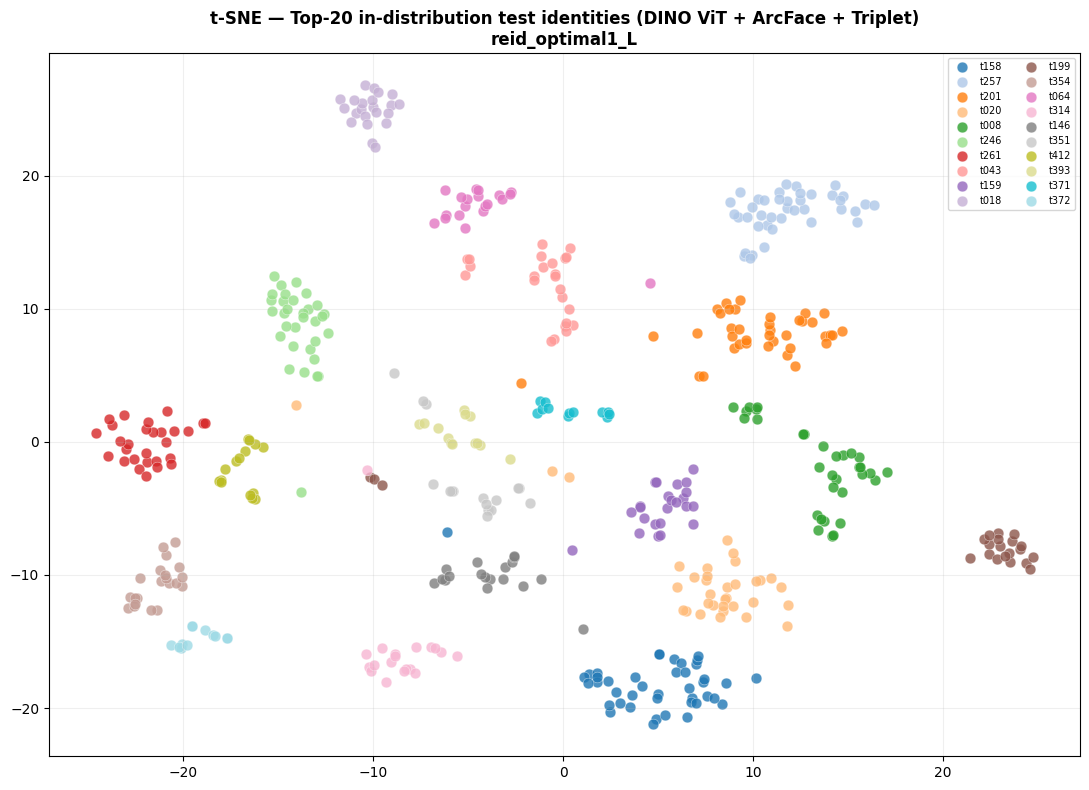
\includegraphics[width=0.85\textwidth]{bab4/tsne2.png}
    \caption{Visualisasi t-SNE untuk 20 identitas penyu teratas pada data pengujian \textit{in-distribution} dengan konfigurasi kombinasi. Setiap warna mewakili satu identitas.}
    \label{fig:tsne_kombinasi}
\end{figure}

%% ============================================================
\section{Pengujian Generalisasi Lintas-Dataset pada SeaTurtleID2022}
\label{sec:pengujian_cross_dataset}
%% ============================================================

%% PERINGATAN: prosedur di bawah kini single-view (tanpa TTA) agar konsisten dengan
%% Subbab protokol evaluasi. Seluruh angka dan gambar bagian ini masih berasal dari run
%% ber-TTA 6-view dan WAJIB di-re-run tanpa TTA sebelum finalisasi:
%% tab:crossdataset_retrieval_only, tab:crossdataset_seaturtleid2022,
%% tab:crossdataset_background_class, tsne3.png, score_dist_threshold.png,
%% score_dist_background.png, cross_query_bottom.png, cross_query_top.png,
%% seluruh rentang skor yang dikutip, dan ROC-AUC 0.77-0.79.

Bagian ini menguji kemampuan generalisasi model ke dataset penyu laut lain di luar
domain pelatihannya. Model dengan \textit{checkpoint} konfigurasi kombinasi
(\textit{backbone} ViT-L/16 DINOv3) diterapkan pada dataset \textbf{SeaTurtleID2022}
tanpa pelatihan ulang. Rangkaian pengujian disusun menaik dari yang paling
mudah ke yang paling menuntut, sehingga setiap tahap mengisolasi satu variabel:

\begin{enumerate}
    \item \textbf{Identifikasi tanpa penolakan.} Seluruh \textit{query} dijamin
          memiliki pasangan di galeri, sehingga yang diuji semata-mata kualitas
          \textit{embedding}.
    \item \textbf{Identifikasi dengan penolakan melalui \textit{threshold} global.}
          Sistem harus menolak \textit{query} dari individu tak terdaftar menggunakan
          satu ambang skor mutlak.
    \item \textbf{Identifikasi dengan penolakan melalui \textit{background class}.}
          Tugas penolakan yang sama, tetapi keputusannya bersifat relatif terhadap
          prototipe individu tak dikenal.
\end{enumerate}

Susunan tersebut memisahkan dua sumber kegagalan yang mungkin terjadi, yaitu apakah
keterbatasan berasal dari kualitas representasi model, atau dari mekanisme pengambilan
keputusan yang bekerja di atas representasi tersebut. Temuan utama seluruh bagian ini
dapat diringkas menjadi tiga poin yang dibuktikan secara berurutan:

\begin{enumerate}
    \item \textbf{Embedding tergeneralisasi dengan penurunan yang terukur.} Pada
          identifikasi tanpa penolakan, model mencapai Rank-1 sebesar 81.1\% dan Rank-5
          sebesar 97.2\% pada dataset baru. Nilai tersebut memang lebih rendah 9.3 poin
          persentase dibanding performa \textit{in-distribution} konfigurasi kombinasi
          (Rank-1 90.4\%), tetapi masih berada pada tingkat yang memadai dan bahkan
          melampaui konfigurasi acuan pada domain aslinya (78.3\%). Kapasitas
          diskriminatif model karenanya bukan merupakan sumber keterbatasan pada skenario
          berpenolakan.
    \item \textbf{Kedua mekanisme penolakan bermuara pada titik operasi yang nyaris
              sama.} Baik \textit{threshold} global sebagai aturan mutlak maupun
          \textit{background class} sebagai aturan relatif menghasilkan
          \textit{trade-off} yang hampir identik, yaitu penolakan individu tak dikenal
          yang nyaris sempurna, dengan konsekuensi penolakan keliru terhadap sekitar
          42\% \textit{query} terdaftar yang valid. Penggantian aturan keputusan hampir
          tidak menggeser titik operasi.
    \item \textbf{Akar persoalan bersifat fundamental pada level skor.} Separabilitas
          skor \textit{registered} terhadap \textit{unregistered} hanya moderat, dengan
          ROC-AUC $\approx 0{.}77$ hingga $0{.}79$. Keterbatasan tersebut membatasi
          seluruh aturan keputusan yang mungkin diterapkan. Aturan relatif yang secara
          rancangan lebih kompleks tidak menghasilkan pemisahan yang lebih baik
          dibandingkan \textit{cosine similarity} sederhana.
\end{enumerate}

\subsection{Prosedur Pengujian}
\label{subsec:openset_prosedur}

Seluruh skenario menggunakan konstruksi galeri dan ekstraksi \textit{embedding} yang
sama, dan perbedaannya hanya terletak pada mekanisme penolakan \textit{unregistered}.

\paragraph{Konstruksi galeri dan query.} Sebanyak 25 identitas dipilih secara acak dari
SeaTurtleID2022 sebagai identitas terdaftar (\textit{registered}). Setiap citra
di-\textit{crop} pada area kepala agar konsisten dengan \textit{preprocessing}
pelatihan. Untuk tiap identitas, 3 citra dipilih secara acak sebagai galeri ($N_G=3$) dan
sisanya menjadi \textit{query}. Galeri disusun per identitas lalu di-\textit{mean-pool}
menjadi satu vektor prototipe yang di-L2-\textit{normalize}. Untuk skenario berpenolakan,
ditambahkan 5 identitas yang sengaja tidak dimasukkan ke galeri (\textit{unregistered}).

\paragraph{Ekstraksi embedding.} Setiap citra diembed dengan \textit{backbone}
ViT-L/16 DINOv3 melalui satu kali lintasan maju atas citra yang telah di-\textit{resize},
kemudian vektor keluarannya di-L2-\textit{normalize}. Prosedur tersebut identik dengan
protokol inferensi pada evaluasi \textit{in-distribution} (Subbab~\ref{subsec:protokol_evaluasi}),
sehingga penurunan performa yang teramati pada bagian ini dapat diatribusikan sepenuhnya
pada pergantian domain, dan bukan pada perbedaan protokol inferensi. \textit{Retrieval}
dihitung dengan \textit{cosine similarity}, dengan opsi \textit{k-reciprocal re-ranking}
($k_1{=}20$, $k_2{=}6$, $\lambda_{\text{rr}}{=}0{.}3$).

\paragraph{Mekanisme penolakan.} Pada skenario berpenolakan, sistem harus memutuskan
apakah sebuah \textit{query} berasal dari identitas terdaftar atau tidak.
\begin{itemize}
    \item \textbf{Threshold global (absolut).} Skor \textit{cosine top-1} terhadap
          galeri dibandingkan terhadap satu ambang tunggal (\textit{Unreg Threshold}).
          Apabila skor berada di bawah ambang, \textit{query} ditandai sebagai
          \textit{Unregistered}. Ambang di-\textit{tune} secara otomatis dengan
          memaksimalkan Youden's J ($\mathit{TPR}-\mathit{FPR}$).
    \item \textbf{Background class (relatif).} Ditambahkan himpunan prototipe
          \textit{background}, yaitu citra penyu di luar 25 identitas galeri, yang
          diambil dari sumber citra terpisah dan dipertahankan sebagai banyak prototipe
          (metode \texttt{samples}, bukan diringkas menjadi satu vektor) agar mewakili
          keragaman individu tak dikenal. Untuk tiap \textit{query} dihitung skor
          keputusan relatif
          \[
              s = s_{\text{reg}} - s_{\text{bg}},
          \]
          yaitu selisih antara kemiripan \textit{top-1} terhadap galeri
          ($s_{\text{reg}}$) dan kemiripan maksimum terhadap prototipe \textit{background}
          ($s_{\text{bg}}$). \textit{Query} diterima sebagai \textbf{Registered} apabila
          $s \geq \textit{margin}$. Karena $s_{\text{bg}}$ dihitung ulang pada setiap
          \textit{query}, skor tersebut menormalisasi \textit{hub identity}, yaitu
          identitas galeri yang mirip terhadap hampir semua citra. \textit{Margin}
          di-\textit{tune} secara otomatis dengan kriteria \texttt{bounded\_frr}
          (\textit{false-reject rate} $\leq 0{.}10$).
\end{itemize}

% VERIFIKASI: pastikan sumber background memang folder terpisah. Bila yang terpakai adalah
% fallback (menyisihkan 50% citra identitas unregistered), jumlah query unregistered pada
% skema background tidak mungkin tetap 49 dan tabel harus dikoreksi.
Karena prototipe \textit{background} diambil dari sumber citra yang terpisah dan tidak
mengambil satu pun citra uji, kedua skema penolakan dievaluasi pada himpunan \textit{query}
yang identik, yaitu 266 citra, sehingga perbandingan keduanya bersifat langsung dan setara.

\subsection{Kualitas Embedding}
\label{subsec:openset_retrieval_only}

Skenario ini hanya berisi 25 identitas terdaftar dan mengasumsikan setiap \textit{query}
pasti memiliki pasangan di galeri, yaitu tanpa individu tak terdaftar dan tanpa mekanisme
penolakan. Hasilnya murni menguji apakah \textit{embedding} model tetap diskriminatif pada
dataset baru.

\begin{table}[H]
    \centering
    \caption{Performa retrieval murni pada query dari identitas terdaftar (tanpa penolakan)}
    \label{tab:crossdataset_retrieval_only}
    \renewcommand{\arraystretch}{1.25}
    \begin{tabular}{lc}
        \hline
        \textbf{Metrik}                     & \textbf{Nilai} \\
        \hline
        Jumlah identitas terdaftar (galeri) & 25             \\
        Citra galeri per identitas ($N_G$)  & 3              \\
        Jumlah \textit{query}               & 217            \\
        Rank-1                              & 81.1\%         \\
        Rank-5                              & 97.2\%         \\
        \hline
    \end{tabular}
\end{table}

Model mencapai Rank-1 sebesar 81.1\% dan Rank-5 sebesar 97.2\% pada dataset yang tidak
digunakan saat pelatihan. Nilai tersebut lebih rendah 9.3 poin persentase dibanding hasil
\textit{in-distribution} konfigurasi kombinasi (Rank-1 90.4\%), sehingga generalisasi
lintas-dataset jelas disertai biaya performa. Namun penurunan tersebut tidak bersifat
katastrofik. Rank-5 sebesar 97.2\% bahkan melampaui Rank-5 \textit{in-distribution}
konfigurasi kombinasi sebesar 96.6\%, dan Rank-1-nya masih berada di atas konfigurasi
acuan pada domain aslinya sebesar 78.3\%. Karena protokol inferensinya identik dengan
evaluasi \textit{in-distribution}, selisih 9.3 poin persentase tersebut dapat
diatribusikan pada pergantian domain semata. Hal ini membuktikan secara langsung bahwa
\textit{embedding} DINOv3 hasil \textit{fine-tuning} tergeneralisasi lintas-dataset.

\begin{figure}[H]
    \centering
    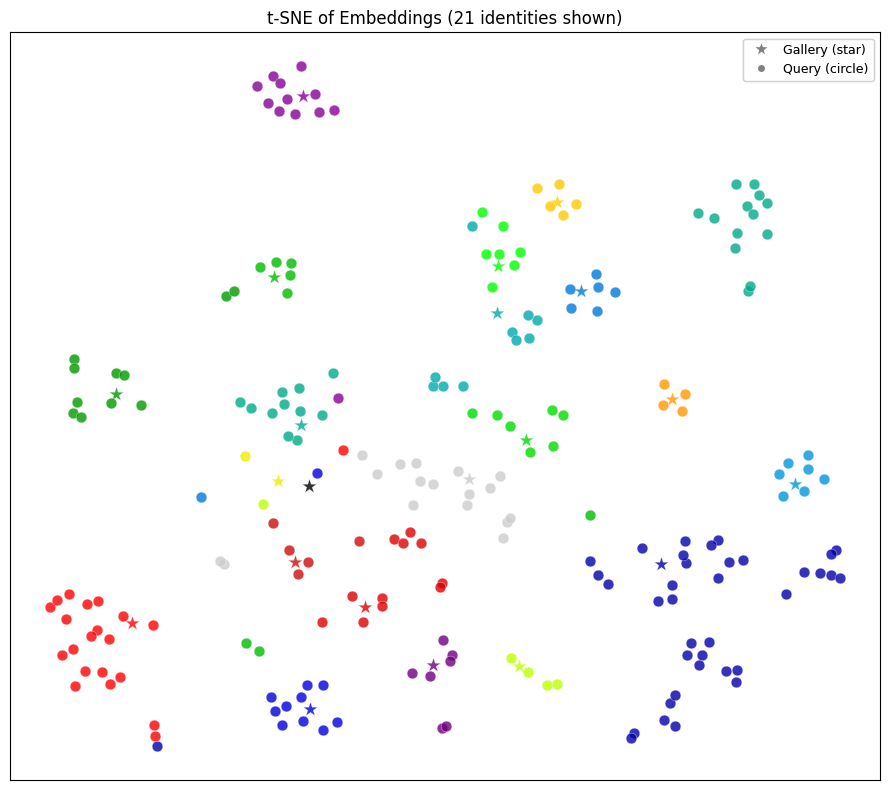
\includegraphics[width=0.85\textwidth]{bab4/tsne3.png}
    \caption{Visualisasi t-SNE vektor \textit{embedding} pada identitas SeaTurtleID2022
        (lintas-dataset, tanpa pelatihan ulang). Bintang menandai prototipe galeri hasil
        \textit{mean-pooling} $N_G=3$ citra, lingkaran menandai citra \textit{query}.
        Setiap warna mewakili satu identitas.}
    \label{fig:tsne_crossdataset}
\end{figure}
% VERIFIKASI: caption lama menyebut 21 identitas, sementara teks menyebut 25 identitas
% terdaftar. Tentukan jumlah identitas yang benar-benar diplot dan cantumkan angkanya.

Gambar~\ref{fig:tsne_crossdataset} memvisualisasikan ruang \textit{embedding} yang
dihasilkan pada dataset lintas-domain tersebut. Struktur yang tampak menjelaskan angka
pada Tabel~\ref{tab:crossdataset_retrieval_only} sekaligus mengantisipasi kegagalan yang
muncul pada skenario berpenolakan.

Klaster tetap terbentuk, tetapi dengan kerapatan yang lebih longgar. Mayoritas identitas
masih membentuk kelompok yang terpisah secara visual dengan prototipe galeri berada di
dalam sebaran \textit{query}-nya sendiri. Struktur inilah yang menopang Rank-1 sebesar
81.1\% dan Rank-5 sebesar 97.2\%. Namun dibandingkan Gambar~\ref{fig:tsne_kombinasi} pada
data \textit{in-distribution}, klaster pada gambar tersebut lebih renggang secara
\textit{intra-class} dan jarak antar-klasternya lebih sempit, konsisten dengan turunnya
Rank-1 dari 90.4\% menjadi 81.1\%. Dengan demikian representasi model tergeneralisasi ke
domain baru, namun disertai penurunan kualitas yang terukur.

\subsection{Identifikasi dengan Penolakan}
\subsubsection{Threshold Global}
\label{subsec:openset_threshold}

Skenario nyata dapat menerima citra individu yang belum pernah didaftarkan. Dengan
penambahan 5 identitas \textit{unregistered}, total \textit{query} menjadi 266, yaitu 217
\textit{registered} dan 49 \textit{unregistered}, dan sistem harus menolak \textit{query}
yang tak terdaftar menggunakan \textit{threshold} global.

\begin{table}[H]
    \centering
    \caption{Hasil identifikasi dengan penolakan pada SeaTurtleID2022 memakai threshold global (25 identitas terdaftar, 5 identitas tidak terdaftar)}
    \label{tab:crossdataset_seaturtleid2022}
    \renewcommand{\arraystretch}{1.25}
    \begin{tabular}{ll}
        \hline
        \textbf{Keterangan}                                          & \textbf{Nilai}                          \\
        \hline
        Jumlah identitas terdaftar (galeri)                          & 25                                      \\
        Citra galeri per identitas ($N_G$)                           & 3                                       \\
        Jumlah identitas tidak terdaftar (baru)                      & 5                                       \\
        \textit{Unregistered threshold} (otomatis, maks. Youden's J) & 0{.}9122                                \\
        Jumlah citra \textit{query}                                  & 266 (terdaftar=217, tidak terdaftar=49) \\
        Akurasi identifikasi                                         & 63.5\%                                  \\
        \textit{Registered} Rank-1 (dengan penolakan)                & 55.3\%                                  \\
        \textit{False-reject rate}                                   & 43.4\%                                  \\
        \textit{Unregistered recall}                                 & 100.0\%                                 \\
        \textit{False-accept rate}                                   & 0.0\%                                   \\
        \hline
    \end{tabular}
\end{table}

Ketika penolakan diaktifkan, \textit{Registered} Rank-1 turun dari 81.1\% pada skenario
tanpa penolakan menjadi 55.3\%. Penurunan tersebut bukan merupakan akibat memburuknya
\textit{embedding}, karena kemampuan \textit{ranking} model tidak berubah sama sekali di
antara kedua skenario. Yang berubah hanyalah keberadaan mekanisme penolakan yang
ditempatkan sebelum proses \textit{ranking}. Sumbernya terbaca jelas dari FRR sebesar
43.4\%, yaitu hampir separuh \textit{query} yang sebenarnya terdaftar ditolak sebagai
\textit{Unregistered} sebelum sempat diperingkat.

\begin{figure}[H]
    \centering
    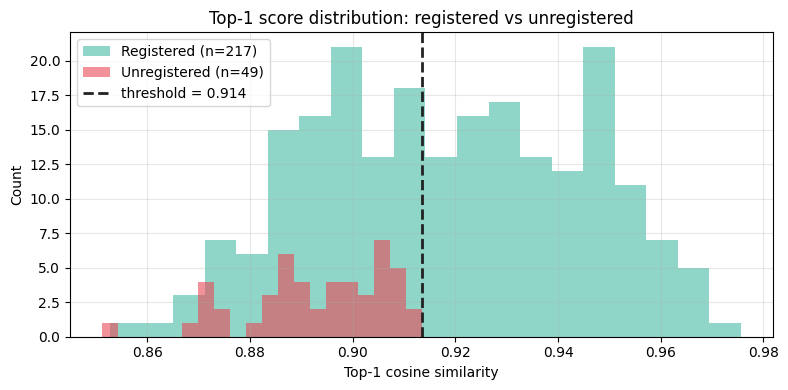
\includegraphics[width=\textwidth]{bab4/score_dist_threshold.png}
    \caption{Distribusi skor \textit{top-1 cosine similarity} terhadap galeri untuk
        \textit{query} terdaftar ($n=217$) dan tidak terdaftar ($n=49$) pada
        SeaTurtleID2022. Garis putus-putus menandai ambang penolakan hasil
        penyetelan otomatis (maks. Youden's J).}
    \label{fig:score_dist_threshold}
\end{figure}

Gambar~\ref{fig:score_dist_threshold} memperlihatkan distribusi skor yang menjadi dasar
seluruh keputusan penolakan pada skema tersebut. Angka-angka pada
Tabel~\ref{tab:crossdataset_seaturtleid2022} merupakan konsekuensi geometris yang dapat
dibaca langsung dari gambar tersebut.

Seluruh skor, baik terdaftar maupun tidak,
terkurung dalam pita $\approx 0{.}85$ hingga $0{.}98$, dan tidak terdapat satu pun
\textit{query} yang skor \textit{top-1}-nya jatuh di bawah 0.85. Artinya, sebuah citra
penyu yang identitasnya sama sekali tidak ada di galeri tetap memperoleh kemiripan
\textit{cosine} sekitar 0.90 terhadap prototipe individu lain. Konsentrasi tersebut
berasal dari struktur data itu sendiri, yaitu seluruh citra berbagi struktur yang nyaris
identik berupa kepala penyu pada latar bawah air, sehingga \textit{embedding} menempati
kerucut sempit pada \textit{hypersphere} dan kemiripan \textit{cosine} antara dua citra
sembarang sudah tinggi sebelum informasi identitas ikut diperhitungkan. Konsekuensinya,
sinyal diskriminatif yang tersedia bagi mekanisme penolakan hanya menempati rentang
selebar $\approx 0{.}13$, jauh lebih sempit dari rentang teoretis \textit{cosine}.

Pola pada
gambar tersebut bukan berupa dua distribusi yang bergeser dan bertumpang tindih pada
tepinya, melainkan distribusi \textit{unregistered} yang seluruhnya tertanam di dalam ekor
bawah distribusi \textit{registered}. Tidak terdapat satu pun \textit{query} tak terdaftar
yang melampaui ambang, sehingga FAR sebesar 0.0\% dan \textit{unregistered recall} sebesar
100.0\% pada Tabel~\ref{tab:crossdataset_seaturtleid2022} dapat diperkirakan sebelumnya,
karena ambang memang ditempatkan tepat pada batas atas sebaran skor mereka. Perlu
ditekankan bahwa \textit{recall} sebesar 100.0\% tersebut diperoleh dari hanya 49
\textit{query} tak terdaftar dan pada ambang yang di-\textit{tune} pada himpunan yang sama,
sehingga tidak dapat dibaca sebagai jaminan penolakan sempurna pada data baru. Karena
distribusi \textit{registered} juga menempati pita yang sama, setiap ambang yang cukup
tinggi untuk menyingkirkan seluruh \textit{unregistered} pasti ikut menyingkirkan sebagian
besar \textit{registered}. FRR sebesar 43.4\% karenanya merupakan konsekuensi langsung dari
struktur distribusi tersebut, dan bukan akibat penyetelan ambang yang keliru.

Kriteria
$J=\mathit{TPR}-\mathit{FPR}$ menyeimbangkan proporsi ternormalisasi, dan bukan cacah
mentah. Pada pita tumpang tindih $\approx 0{.}88$ hingga $0{.}91$, meskipun cacah
\textit{registered} per \textit{bin} tampak lebih tinggi secara visual, mayoritas dari
hanya 49 \textit{query} tak terdaftar terkonsentrasi pada pita tersebut, sementara 217
\textit{query} terdaftar tersebar hingga 0.98. Kerapatan ternormalisasi
\textit{unregistered} pada pita tersebut karenanya lebih tinggi daripada
\textit{registered}. Setiap penurunan ambang di wilayah tersebut menambah FPR lebih cepat
daripada menambah TPR, sehingga $J$ maksimum tercapai persis pada titik FPR $=0$. Optimum
tersebut bersifat \textit{corner solution}, yaitu terpilih bukan karena merupakan kompromi
yang baik, melainkan karena tidak tersedia kompromi yang lebih baik.

\subsubsection{Background Class}
\label{subsec:openset_background}

Pendekatan \textit{threshold} bersifat \textit{post-hoc}, yaitu satu ambang mutlak di atas
skor \textit{cosine} yang terpisah dari proses \textit{retrieval}. Sebagai alternatifnya,
penolakan dijadikan bagian dari kompetisi \textit{retrieval} itu sendiri melalui
\textit{background class}, yaitu sebuah \textit{query} ditolak apabila prototipe
\textit{background} mengungguli kandidat galeri terbaiknya
($s = s_{\text{reg}} - s_{\text{bg}} < \textit{margin}$).

\begin{table}[H]
    \centering
    \caption{Hasil identifikasi dengan penolakan memakai penambahan background class pada galeri}
    \label{tab:crossdataset_background_class}
    \renewcommand{\arraystretch}{1.25}
    \begin{tabular}{ll}
        \hline
        \textbf{Keterangan}                                     & \textbf{Nilai}                          \\
        \hline
        Jumlah identitas terdaftar (galeri)                     & 25                                      \\
        Citra galeri per identitas ($N_G$)                      & 3                                       \\
        Metode prototipe                                        & \texttt{samples}                        \\
        \textit{Margin} keputusan (auto, \texttt{bounded\_frr}) & $+0{.}0148$                             \\
        Jumlah citra \textit{query}                             & 266 (terdaftar=217, tidak terdaftar=49) \\
        Akurasi identifikasi                                    & 64.3\%                                  \\
        \textit{Registered} Rank-1 (dengan penolakan)           & 56.7\%                                  \\
        \textit{False-reject rate}                              & 41.9\%                                  \\
        \textit{Unregistered recall}                            & 98.0\%                                  \\
        \textit{False-accept rate}                              & 2.0\%                                   \\
        \hline
    \end{tabular}
\end{table}

Temuan paling penting dari skema tersebut bukanlah keunggulannya, melainkan kemiripannya
dengan \textit{threshold} global. Karena kedua skema dievaluasi pada himpunan
\textit{query} yang identik sebanyak 266 citra, perbandingannya bersifat langsung.
Meskipun mekanismenya berbeda secara fundamental, yaitu mutlak berbanding relatif,
\textit{background class} bermuara pada titik operasi yang nyaris sama, yaitu
\textit{Registered} Rank-1 sebesar 56.7\% berbanding 55.3\%, FRR sebesar 41.9\% berbanding
43.4\%, \textit{unregistered recall} sebesar 98.0\% berbanding 100.0\%, dan FAR sebesar
2.0\% berbanding 0.0\%. Akurasi identifikasi keduanya pun berdekatan, yaitu 64.3\%
berbanding 63.5\%. Seluruh selisih tersebut berada pada orde satu hingga dua
\textit{query}. Skema relatif tersebut karenanya tidak membuka \textit{trade-off} yang
lebih baik, melainkan hanya mencapai titik operasi yang sama ketatnya melalui jalan yang
berbeda.

Konsistensi tersebut sekali lagi menegaskan bahwa \textit{embedding} tidak pernah menjadi
sumber masalah. Efek seleksi yang sama juga muncul, yaitu di antara \textit{query}
terdaftar yang lolos, akurasi \textit{retrieval} mencapai $0{.}567/(1-0{.}419) \approx
    97{.}6\%$, praktis identik dengan $\approx 97{.}7\%$ pada \textit{threshold} global.
Kedua mekanisme penolakan sama-sama ketat, sehingga sama-sama menyingkirkan kasus sulit
terlebih dahulu dan menyisakan subset \textit{query} yang relatif mudah.

\begin{figure}[H]
    \centering
    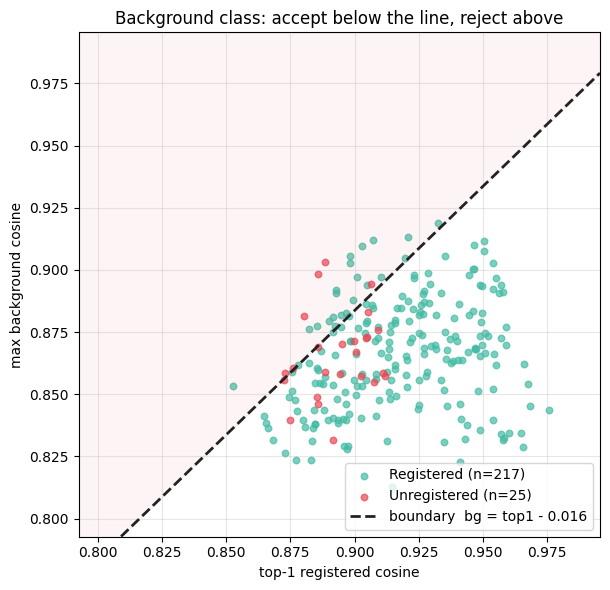
\includegraphics[width=0.8\textwidth]{bab4/score_dist_background.png}
    \caption{Ruang keputusan \textit{background class} pada SeaTurtleID2022. Sumbu
        horizontal menyatakan kemiripan \textit{top-1} terhadap prototipe galeri
        ($s_{\text{reg}}$), sumbu vertikal menyatakan kemiripan maksimum terhadap
        prototipe \textit{background} ($s_{\text{bg}}$). Garis putus-putus adalah batas
        keputusan $s_{\text{bg}} = s_{\text{reg}} - \textit{margin}$; \textit{query} di
        bawah garis diterima sebagai \textit{Registered}, di atas garis ditolak.}
    \label{fig:bg_class_scatter}
\end{figure}

Gambar~\ref{fig:bg_class_scatter} memplot kedua komponen skor keputusan secara terpisah,
sehingga dapat diperiksa berapa besar kontribusi masing-masing terhadap keputusan akhir.
Dari gambar tersebut dapat dibaca alasan mengapa skema relatif ini bermuara pada titik
operasi yang nyaris identik dengan \textit{threshold} global.

Sumbu vertikal tidak membawa informasi diskriminatif. Perbandingan sebaran kedua kelas
pada masing-masing sumbu bersifat menentukan. Pada sumbu horizontal, \textit{query} tak
terdaftar terkonsentrasi pada pita $s_{\text{reg}} \approx 0{.}85$ hingga $0{.}915$
sementara \textit{query} terdaftar terbentang hingga $\approx 0{.}975$, sehingga pemisahan
antar-kelas terjadi di sepanjang sumbu tersebut, persis seperti pada
Gambar~\ref{fig:score_dist_threshold}. Sebaliknya, pada sumbu vertikal kedua kelas
menempati rentang yang praktis berimpit, yaitu $s_{\text{bg}} \approx 0{.}83$ hingga
$0{.}92$, dengan pemusatan yang nyaris sama. Nilai $s_{\text{bg}}$ juga tidak menunjukkan
ketergantungan yang kuat terhadap $s_{\text{reg}}$, karena untuk hampir seluruh rentang
$s_{\text{reg}}$ sebaran $s_{\text{bg}}$ tetap serupa. Dengan demikian $s_{\text{bg}}$
tidak membawa informasi mengenai apakah sebuah \textit{query} terdaftar atau tidak. Skor
keputusan $s = s_{\text{reg}} - s_{\text{bg}}$ karenanya secara efektif merupakan
$s_{\text{reg}}$ yang ditambahi komponen derau, dan hal inilah yang menyebabkan aturan
relatif tersebut bermuara pada titik operasi yang sama dengan aturan mutlak.

\subsection{Analisis Kualitatif Lintas Dataset}
Gambar~\ref{fig:cross_query_bottom} dan Gambar~\ref{fig:cross_query_top} menampilkan lima
keputusan paling keliru dan lima keputusan paling tepat pada skema
\textit{background class}, lengkap dengan lima kandidat galeri teratas beserta skor
\textit{cosine}-nya.

\begin{figure}[H]
    \centering
    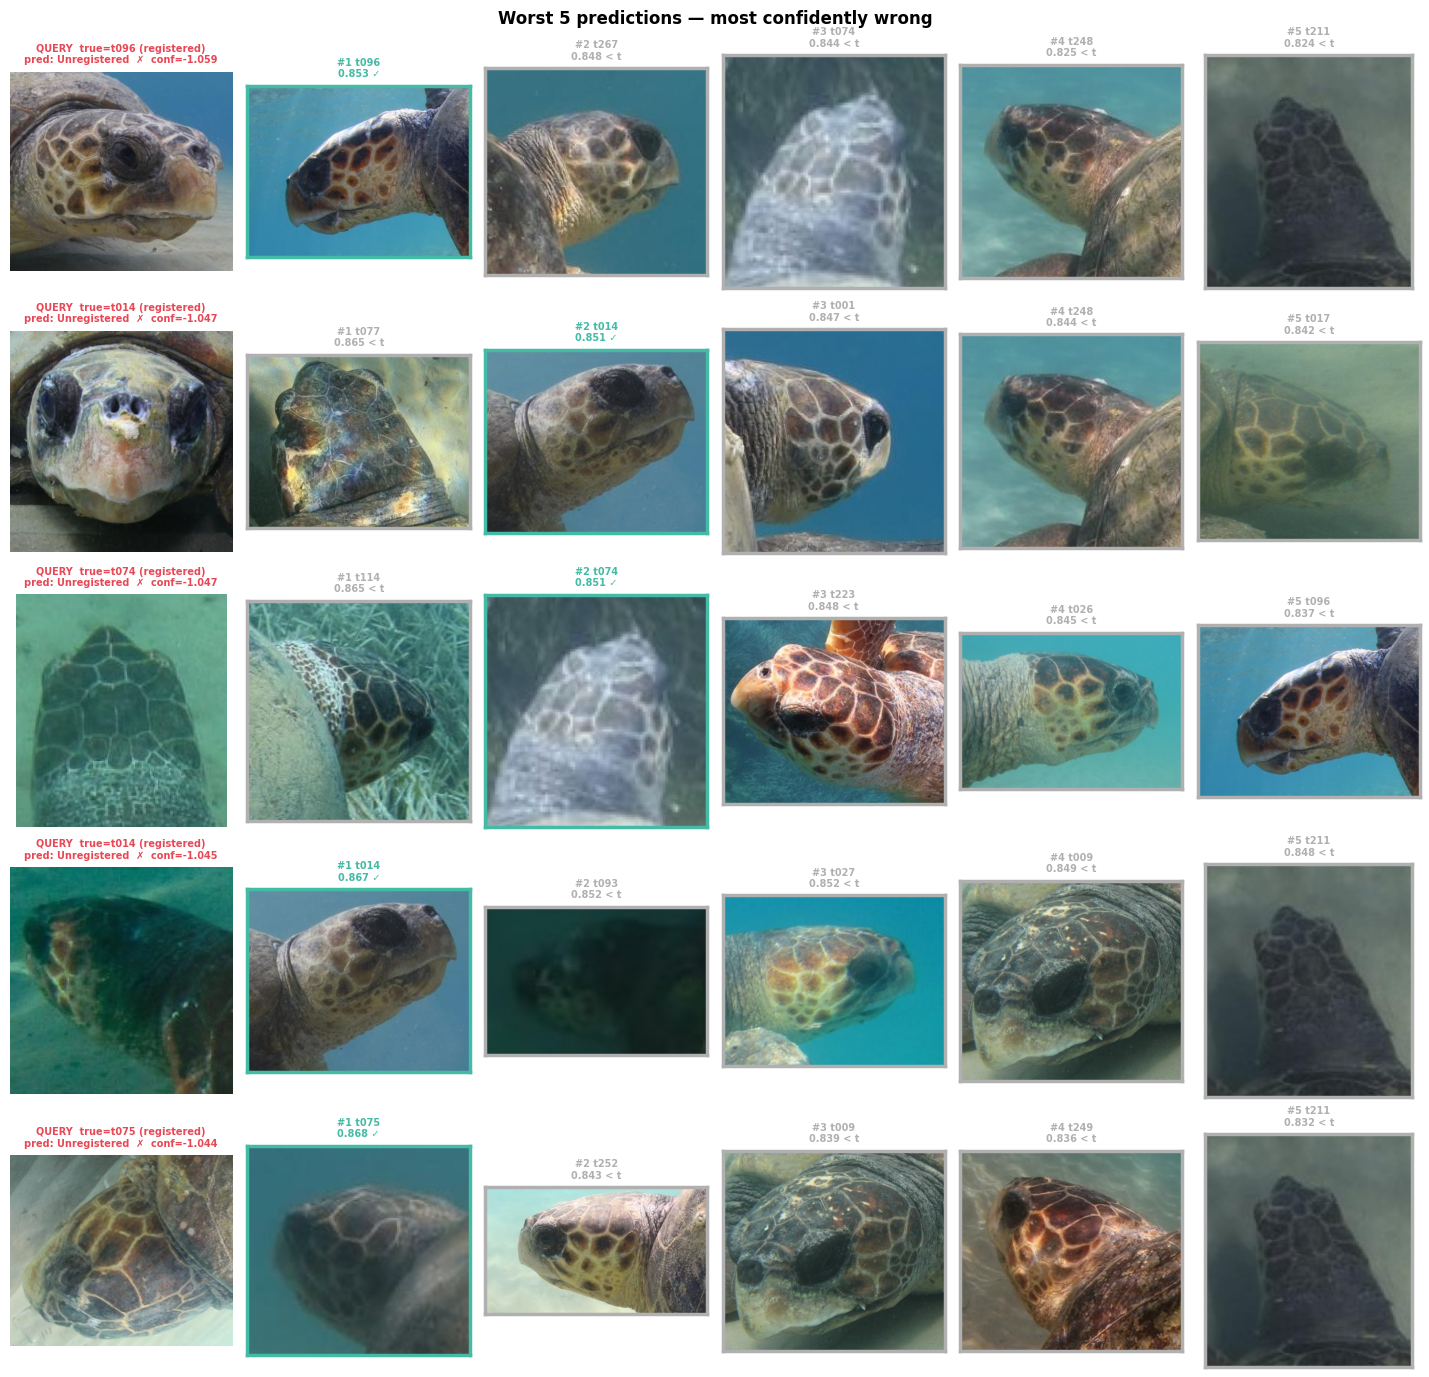
\includegraphics[width=\textwidth]{bab4/cross_query_bottom.png}
    \caption{Lima keputusan paling keliru pada skema \textit{background class}
        (SeaTurtleID2022). Kolom pertama adalah citra \textit{query} beserta identitas
        sebenarnya dan prediksi sistem; kolom berikutnya adalah lima kandidat galeri
        teratas terurut menurun berdasarkan \textit{cosine similarity}. Penanda hijau
        menunjukkan kandidat dengan identitas yang benar.}
    \label{fig:cross_query_bottom}
\end{figure}

\begin{figure}[H]
    \centering
    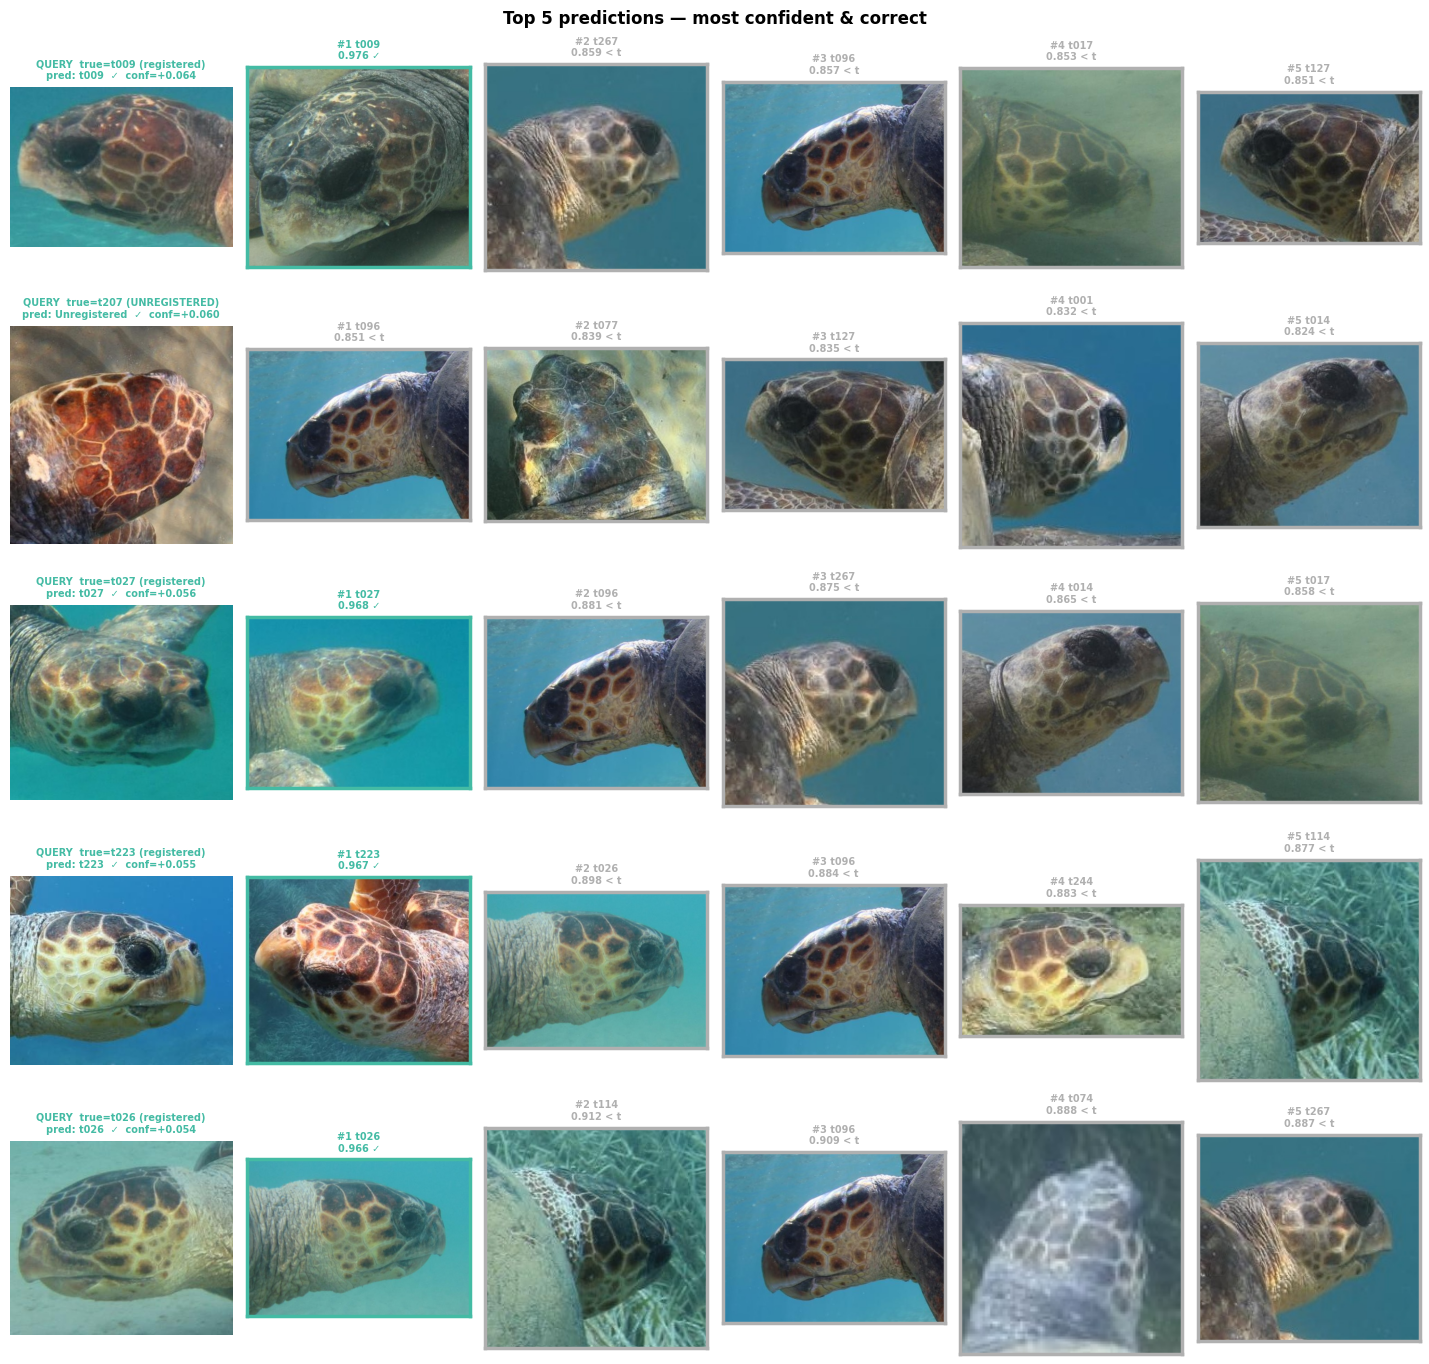
\includegraphics[width=\textwidth]{bab4/cross_query_top.png}
    \caption{Lima keputusan paling tepat pada skema \textit{background class}
        (SeaTurtleID2022), dengan konvensi penyajian yang sama dengan
        Gambar~\ref{fig:cross_query_bottom}.}
    \label{fig:cross_query_top}
\end{figure}

Dua hal dapat dianalisis dari Gambar~\ref{fig:cross_query_bottom}, dan keduanya memperkuat
kesimpulan bahwa keterbatasan sistem terletak pada mekanisme keputusan, dan bukan pada
representasi.

Pertama, kelima kegagalan terparah merupakan \textit{query} dari identitas terdaftar
yang ditolak sebagai \textit{Unregistered}, dan tidak satu pun di antaranya merupakan
\textit{false accept}. Komposisi tersebut merupakan wujud visual dari asimetri pada
Tabel~\ref{tab:crossdataset_background_class}, yaitu FRR sebesar 41.9\% berhadapan dengan
FAR sebesar 2.0\%. Kegagalan mekanisme penolakan karenanya tidak bersifat simetris,
melainkan hampir seluruhnya terjadi pada satu arah.

Kedua, dan yang paling menentukan, pada kelima kasus tersebut identitas yang benar tetap
berada di dalam lima kandidat teratas, bahkan tepat pada peringkat-1 untuk tiga di
antaranya, yaitu t096 dengan skor 0.853, t014 dengan skor 0.867, dan t075 dengan skor
0.868. Pada kasus yang secara kuantitatif tergolong paling parah sekalipun, proses
\textit{retrieval} sesungguhnya telah menempatkan jawaban yang benar pada posisi teratas,
dan keputusan penolakanlah yang kemudian membuangnya sebelum peringkat tersebut sempat
dilaporkan. Temuan tersebut menutup kemungkinan bahwa penurunan \textit{Registered} Rank-1
dari 81.1\% menjadi 56.7\% berasal dari melemahnya kualitas \textit{embedding} pada domain
baru.

Perbandingan dengan Gambar~\ref{fig:cross_query_top} memperlihatkan alasan mengapa
mekanisme penolakan tersebut tidak dapat disetel lebih longgar. Keputusan yang tepat
ditandai skor \textit{top-1} pada rentang 0.966 hingga 0.976, terpisah jelas dari kandidat
kedua yang berada di sekitar 0.86 hingga 0.91. Sebaliknya, penolakan yang benar terhadap
identitas tak terdaftar (t207) terjadi ketika skor \textit{top-1}-nya hanya mencapai 0.851.
Perbandingan inilah yang menjadi inti persoalan. Pada kasus gagal di
Gambar~\ref{fig:cross_query_bottom}, skor pencocokan yang benar berada pada rentang 0.851
hingga 0.868, yaitu berimpit dengan skor \textit{top-1} milik \textit{query} t207 yang
identitasnya sama sekali tidak ada di galeri. Sebuah pencocokan yang benar dan sebuah
\textit{query} yang sepenuhnya asing karenanya menghasilkan skor yang praktis tidak dapat
dibedakan. Sistem hanya dapat memutuskan dengan andal ketika \textit{query} memiliki
pasangan galeri berpose serupa yang menghasilkan skor di atas $\approx 0{.}95$, sedangkan
di luar kondisi tersebut seluruh kasus terkonsentrasi pada pita 0.84 hingga 0.88 yang sama.
Inilah dasar konkret dari ROC-AUC $\approx 0{.}77$ hingga $0{.}79$ yang membatasi seluruh
aturan keputusan, sekaligus alasan mengapa penggantian aturan keputusan dari mutlak menjadi
relatif tidak menggeser titik operasi.
\cleardoublepage
\chapter{PENUTUP}

\section{Kesimpulan}

Model re-identifikasi penyu berbasis \textit{backbone} Vision Transformer pra-latih DINOv3
dengan pendekatan \textit{metric learning} mampu mengenali individu penyu dari pola kepalanya pada
skenario \textit{open-set}. Konfigurasi acuan memperoleh Rank-1 sebesar 78,3\% dan mAP sebesar
84,9\%, sedangkan konfigurasi kombinasi memperoleh Rank-1 sebesar 90,4\% dan mAP sebesar 93,5\%.
Penerapan \textit{k-reciprocal re-ranking} hanya menambah 0,9 hingga 1,3 poin persentase. Sebagian
besar kegagalan berupa kesalahan pengurutan pada peringkat teratas, bukan kegagalan menemukan
identitas yang benar. Kegagalan tersebut umumnya terjadi pada citra yang buram dan berkontras
rendah.

Model mampu bergeneralisasi ke data dengan kondisi pengambilan citra yang berbeda. Tanpa
pelatihan ulang, model memperoleh Rank-1 sebesar 81,1\% dan Rank-5 sebesar 97,2\% pada dataset
SeaTurtleID2022. Performanya turun 9,3 poin persentase dari hasil \textit{in-distribution}.
Protokol inferensi pada kedua pengujian identik, sehingga penurunan tersebut murni bersumber dari
pergantian domain. Dengan demikian, generalisasi model disertai biaya performa yang terukur dan
tidak katastrofik.

Penanganan identitas tidak terdaftar merupakan keterbatasan utama sistem. Nilai Registered
Rank-1 turun menjadi 55,3\% pada skema \textit{threshold} global dan 56,7\% pada skema
\textit{background class}, dengan \textit{false-reject rate} sekitar 42\%. Aturan keputusan kedua
skema berbeda secara fundamental, tetapi keduanya bermuara pada titik operasi yang nyaris sama.
Penyebabnya terletak pada distribusi skor. Seluruh skor \textit{top-1} terkurung dalam pita sempit
0,85 hingga 0,98, dan distribusi \textit{unregistered} tertanam di dalam distribusi
\textit{registered}, sehingga separabilitasnya hanya moderat dengan ROC-AUC 0,77 hingga 0,79.
Meskipun demikian, identitas yang benar tetap berada pada lima kandidat teratas bahkan pada kasus
kegagalan terparah. Keterbatasan sistem karenanya bersumber dari mekanisme keputusan dan kalibrasi
skor, bukan dari kualitas \textit{embedding}.


\section{Saran}

Berdasarkan keterbatasan yang teridentifikasi, terdapat beberapa saran yang dapat dipertimbangkan
untuk penelitian selanjutnya, yaitu sebagai berikut.

\begin{enumerate}

    \item Pendekatan \textit{one-factor-at-a-time} perlu didukung dengan rancangan faktorial atau
          ablasi mundur dari konfigurasi kombinasi. Sub-aditivitas yang terbukti pada Subbab 4.4.7
          menunjukkan bahwa penggabungan seluruh nilai terbaik tidak menjamin tercapainya optimum.

    \item Eksperimen perlu dijalankan menggunakan beberapa \textit{seed} yang berbeda. Seluruh hasil
          pada penelitian ini berasal dari satu \textit{seed} tunggal. Akibatnya, parameter dengan rentang
          di bawah 2 poin persentase tidak dapat disimpulkan tanpa estimasi variansi antar-\textit{seed}.
          Pelaporan dalam bentuk rata-rata dan simpangan baku akan memisahkan efek yang nyata dari
          fluktuasi acak.

    \item Penyetelan ambang penolakan perlu dilakukan pada himpunan validasi yang
          terpisah dari himpunan evaluasi. Jumlah identitas tidak terdaftar juga perlu
          diperbesar.

    \item Kemiripan antara profil kiri dan profil kanan penyu dapat dieksploitasi sebagaimana
          diusulkan pada penelitian terdahulu. Pemanfaatannya berpotensi menambah jumlah data yang tersedia
          untuk pencocokan tanpa memerlukan pengumpulan citra baru.

    \item Tahap deteksi dan segmentasi kepala dapat diintegrasikan sehingga terbentuk
          \textit{pipeline} \textit{end-to-end}. Penelitian ini mengasumsikan citra masukan telah
          ter-\textit{crop} pada region kepala. Penggabungan tahap deteksi akan menghasilkan alur kerja yang
          dapat langsung diterapkan pada foto lapangan mentah.

\end{enumerate}
\cleardoublepage
\input{Init/DaftarPustaka.tex}
\cleardoublepage
\begin{center}
  \Large
  \textbf{BIOGRAFI PENULIS}
\end{center}

\addcontentsline{toc}{chapter}{BIOGRAFI PENULIS}

\vspace{2ex}

\begin{wrapfigure}{L}{0.3\textwidth}
  \centering
  \vspace{-3ex}
  % Ubah file gambar berikut dengan file foto dari mahasiswa
  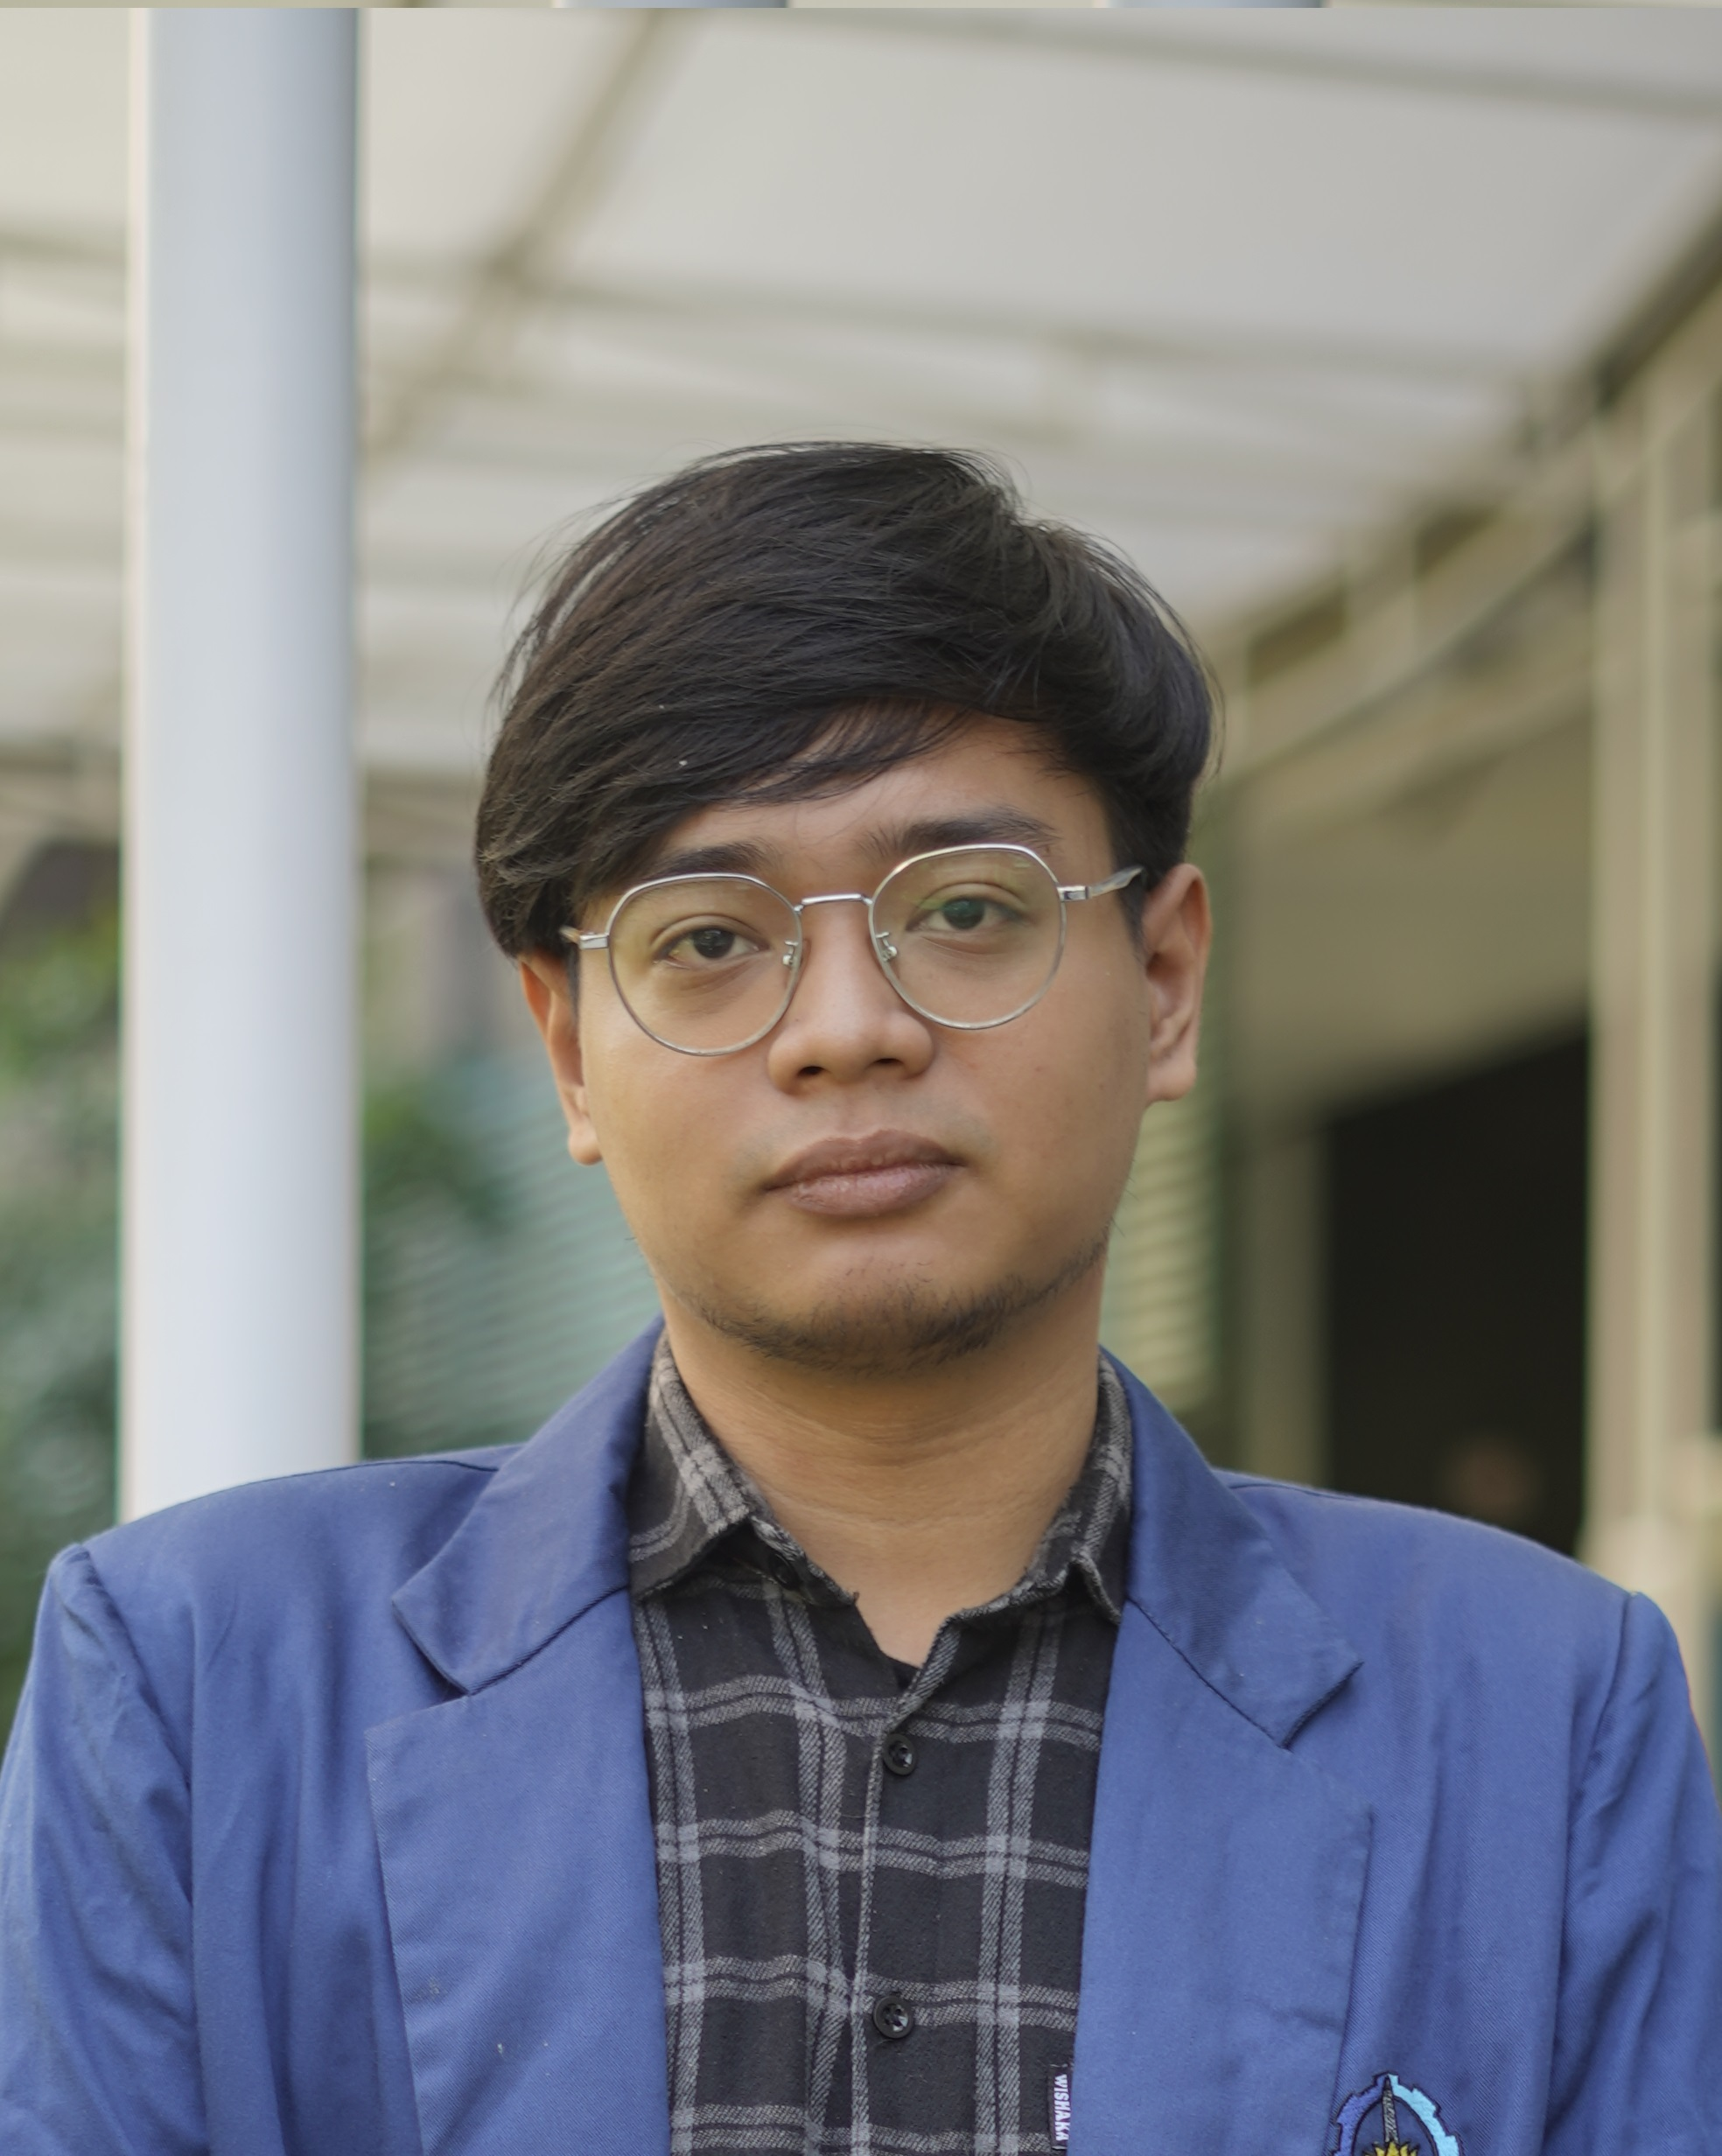
\includegraphics[width=0.3\textwidth]{BiografiPenulis/foto-formal.jpg}
  \vspace{-4ex}
\end{wrapfigure}

Sulthan Daffa Arif Mahmudi atau yang lebih akrab disapa Daffa Lahir di Lamongan pada tanggal 30 Juli 2003. Ia merupakan anak kedua dari dua bersaudara. Penulis lulus dari SMAN 2 Lamongan dalam waktu 2 tahun, dan melanjutkan pendidikan ke strata satu Teknik Komputer di Institut Sepuluh Nopember Surabaya.

Pilihan ini bukan tanpa alasan, sejak awal ia memiliki ketertarikan dalam \textit{game development} memperkuat pilihannya di fakultas tersebut.
Semasa awal perkuliahan ia aktif mengikuti berbagai macam kegiatan. Pada tahun pertama, ia telah mendapatkan kesempatan untuk mengikuti proyek yang melibatkan pengembangan aplikasi dan web di luar lingkungan akademik.
Pada tahun kedua dan ketiganya disibukkan dengan penelitian pada tim robotik Bayucaraka ITS dengan posisi \textit{electro-programmer} pada divisi \textit{flight controller}. Ia telah membantu mengembangkan \textit{firmware} untuk kontroller penerbangan pesawat dan drone yang telah digunakan pada Kompetisi Robot Terbang Indonesia (KRTI).

Pada tahun perkuliahannya, ia telah mengusulkan tiga judul PKM, yang di mana dua di antaranya telah mendapatkan pendanaan. Selain itu, ia juga terlibat dengan beberapa riset pada Departemen Teknik Komputer itu sendiri. Selain itu juga terdapat banyak proyek di luar lingkungan akademik yang pernah ia jalani, dari game, aplikasi, web, dan editor yang membantu memperluas portofolionya.

Dibalik latar belakang teknik dan IT tersebut, Daffa juga memiliki hobi menulis dan mengarang. Ketertarikannya terhadap \textit{character design} dan \textit{worldbuilding} juga menimbulkan hobi menggambar. Semua hobi ini pada akhirnya berujung ke ketertarikannya pada \textit{game development}.
\cleardoublepage
\end{document}
